
% LTeX: language=fr
%%%%%%%%%%%%%%%%%%%%%%%%%%%%%%%%%%%%%%%%%%%%%%%%%%%%%%%%%%%%%%%%%%%%%%%%%%
%%%%%                         CHAPITRE 2
%%%%%%
%%%%%%%%%%%%%%%%%%%%%%%%%%%%%%%%%%%%%%%%%%%%%%%%%%%%%%%%%%%%%%%%%%%%%%%%%%

\lhead[\fancyplain{}{\leftmark}]%Pour les pages paires \bfseries
      {\fancyplain{}{}} %Pour les pages impaires
\chead[\fancyplain{}{}]%
      {\fancyplain{}{}}
\rhead[\fancyplain{}{}]%Pour les pages paires 
      {\fancyplain{}{\rightmark}}%Pour les pages impaires \bfseries
\lfoot[\fancyplain{}{}]%
      {\fancyplain{}{}}
\cfoot[\fancyplain{}{\thepage}]%\bfseries
      {\fancyplain{}{\thepage}} %\bfseries
\rfoot[\fancyplain{}{}]%
     {\fancyplain{}{\scriptsize}}

\def \hfillx {\hspace*{ -\textwidth} \hfill} % remplir espacement horizontal entre deux sous-figures de façon à remplir toute la largeur du texte.
\raggedbottom 
%%%%%%%%%%%%%%%%%%%%%%%%%%%%%%%%%%%%%%%%%%%%%%%%%%%%%%%%%%%%%%%%%%%%%%%%%%
%%%%%                      Start part here                          %%%%%%
%%%%%%%%%%%%%%%%%%%%%%%%%%%%%%%%%%%%%%%%%%%%%%%%%%%%%%%%%%%%%%%%%%%%%%%%%%

\chapter{Modélisation et simulation du système de récupération d’énergie intra-auriculaire}
\label{ch:2_Modelisation et simulation du systeme}

\minitoc
\newpage

%/!\/!\/!\/!\/!\/!\/!\/!\/!\/!\/!\/!\/!\/!\/!\/!\/!\/!\/!\/!\/!\/!\/!\/!\%
\section{Solution proposée pour maximiser l'énergie récupérée}
\label{sec:2.1_Solution proposee pour maximiser l energie recuperee}
%/!\/!\/!\/!\/!\/!\/!\/!\/!\/!\/!\/!\/!\/!\/!\/!\/!\/!\/!\/!\/!\/!\/!\/!\%
		%////////////////////////////////////////////
		\subsection{Pertinence de la chaîne de conversion d’énergie envisagée}
		\label{subsec:2.1.1_Pertinence de la chaine de conversion d energie envisagee}
		%////////////////////////////////////////////
\lettrine[lines=1]{E~}{}n considérant l'état de l'art en matière de technologies de récupération d'énergie, ainsi que de la nature peu commune de la source d'énergie, impliquant les tissus mous du corps humain, la faible fréquence de mastication et le faible volume offert par le CA, nous proposons une nouvelle stratégie de conversion d'énergie. La chaîne de conversion énergétique de notre solution est présentée sur la figure \ref{fig:conversion_symme}.
%%%%%%%%%%%%%%%%%%%%		
\begin{figure}[!htbp]
	\begin{center}
		\captionsetup{justification=centering}
		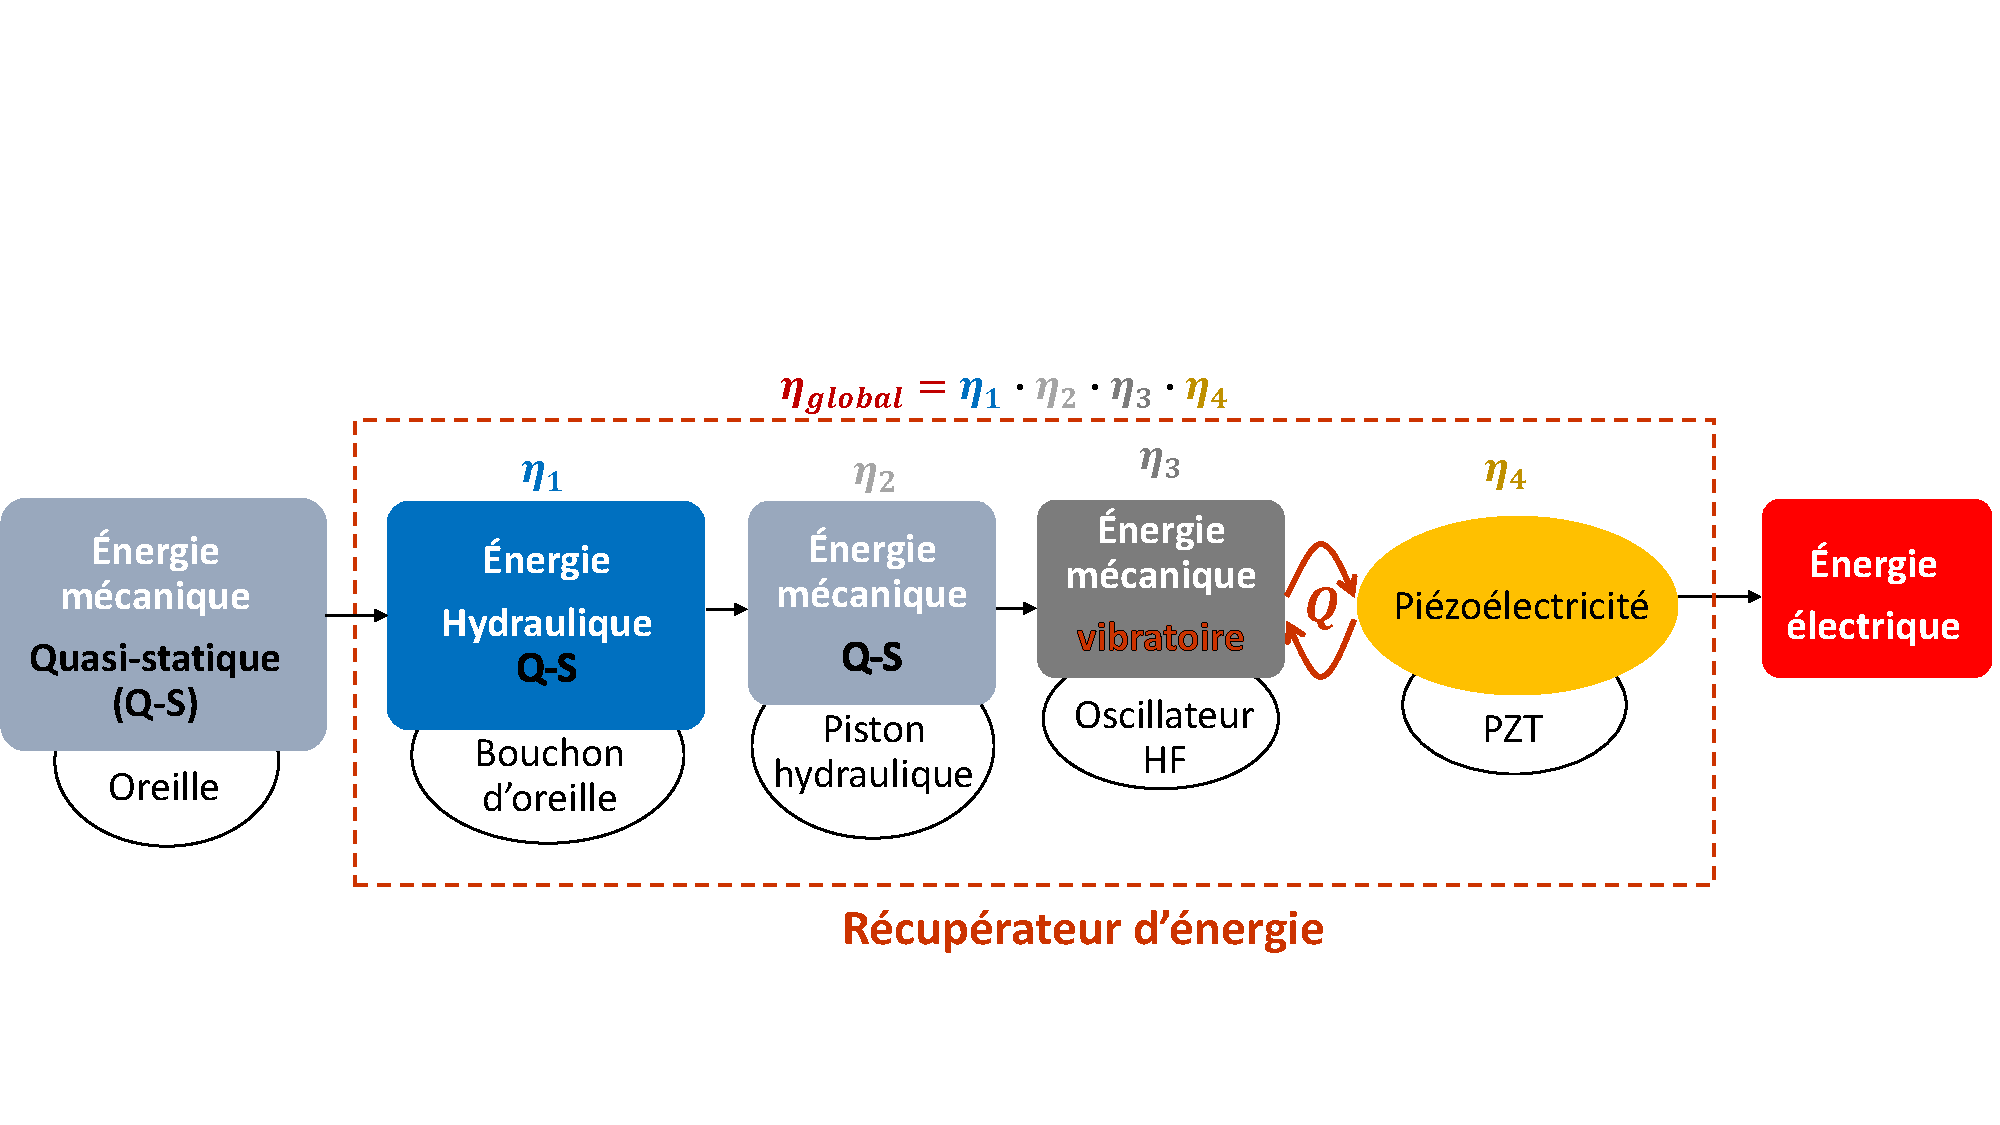
\includegraphics[trim={0cm 2.5cm 0cm 6cm},clip,width=\textwidth]{../Chap2/Figure/conversion_symme.pdf}
		\caption{Chaîne de conversation envisagée dans ces travaux}
		\label{fig:conversion_symme}
	\end{center}
\end{figure}
%%%%%%%%%%%%%%%%%%%%

On propose un nombre d'étapes de conversion supérieur aux dispositifs présentés précédemment. Bien que le système résultant soit plus complexe, le rendement de conversion au passage de chaque étape est meilleur que celui des solutions présentées dans la littérature. Nous voulons optimiser la chaîne de conversion afin de minimiser les pertes, et, pour ce faire, nous voulons implémenter dans le dispositif les éléments suivants, dont les justifications ont été données précédemment :
\begin{itemize}[label=$\square$]
	\item Une interface de transfert d'énergie hydraulique afin de transférer l'énergie de déformation du canal auditif à l'extérieur de ce-dernier en tirant alors profit d'espace supplémentaire et de faibles pertes énergétiques grâce à l'écoulement à Re<2000. Ce premier sous-système est considéré BF.
	\item La technologie de conversion piézoélectrique qui est la plus efficace à l'échelle de l'application. Des céramiques PZT offriraient par ailleurs un coefficient de couplage électromécanique meilleur que les polymères piézoélectriques type PVDF.
	\item Une structure implémentant des céramiques PZT et un mécanisme oscillant afin d'amplifier la fréquence de l'énergie source et profiter alors du facteur de qualité de ce dernier, offrant un meilleur rendement de conversion que pour un régime quasi-statique. Ce sous-système est considéré HF.
\end{itemize}
On présente alors dans la suite, le détail de l'architecture du récupérateur d'énergie intra-auriculaire développé dans ces travaux, mettant en \oe{}uvre la chaîne de conversion optimisée proposée et maximisant ainsi le rendement du récupérateur.
		%////////////////////////////////////////////
		\subsection{Présentation du système complet}
		\label{subsec:2.1.2_Presentation du systeme complet}
		%////////////////////////////////////////////	
La stratégie adoptée est d'exploiter le bouchon d'oreille comme une pompe hydraulique actionnée par le joint temporo-mandibulaire de la mâchoire lors des phases de mastication. \\
%%%%%%%%%%%%%%%%%%%%%%%%%%%%%%%%%%%%%%%%%%%
\begin{table}[!htbp]
\centering
\rowcolors[]{2}{black!8}{}{
\renewcommand{\arraystretch}{2}
\begin{tabular}{c m{10cm}}
\rowcolor{blue!10}
\toprule
\multicolumn{1}{c}{\textbf{\textit{Composant}}} & \multicolumn{1}{c}{\textbf{Fonction}} \\
\midrule
%%%%%%%%%%%%% Bouchon d'oreille %%%%%%%%%%%%%%%%%%% 
\emph{Bouchon d'oreille} &
Le bouchon d'oreille est rempli de fluide incompressible et \emph{gonflé} à une pression suffisante pour épouser les parois du canal auditif. Il permet alors de capter l'énergie de déformation mécanique du canal auditif et agit comme une mini pompe caractérisée par son débit $q_{ear}$ et sa pression $p_{ear}$.\\  
%%%%%%%%%%%%% OB %%%%%%%%%%%%%%%%%%% 1
\emph{Oscillateur bistable} &
L'oscillateur bistable (OB) permet d'amplifier la fréquence de l'énergie source et offre deux positions stables autour desquels l'oscillation libre de M est possible, après un aller retour du piston hydraulique mettant la masse en mouvement. \\ 
%%%%%%%%%%%%% GPA %%%%%%%%%%%%%%%%%%% 2
\emph{Générateur piézoélectrique} &
Le générateur piézoélectrique amplifié (GPA) permet de convertir l'énergie potentielle élastique accumulée lors du déplacement de la masse en énergie électrique lors des phases d'oscillations. Sa fonction d'amplificateur mécanique est illustrée et modélisée dans cette section. \\ 
%%%%%%%%%%%%% Pistons hydrauliques %%%%%%%%%%%%%%%%%%% 3
\emph{Pistons hydrauliques} &
Les pistons hydrauliques (PH) permettent de convertir l'énergie issue de la pompe hydraulique en travail mécanique lors de leur déplacement. \\ 
%%%%%%%%%%%%% VH %%%%%%%%%%%%%%%%%%%
\emph{Valve hydraulique} &
Les valves hydrauliques (VH) permettent de gérer la direction de l'écoulement en sélectionnant le PH qui sera alimenté par la pompe durant une phase de mastication.\\ 
%%%%%%%%%%%%% Amplificateur hydraulique %%%%%%%%%%%%%%%%%%%
\emph{Amplificateur hydraulique} &
L'amplificateur hydraulique (AH) permet d'adapter l'impédance hydraulique de la mini pompe à l'impédance mécanique de l'OB. \\
%%%%%%%%%%%%% Clapet anti-retour %%%%%%%%%%%%%%%%%%%
\emph{Clapet anti-retour} &
Le clapet anti-retour permettra l'écoulement du fluide depuis le piston vers le bouchon d'oreille lorsque la VH de la branche d'actionnement concernée sera en position fermée.\\
%%%%%%%%%%%%% Découpleur de pression %%%%%%%%%%%%%%%%%%%
\emph{Découpleur hydraulique} &
Le découpleur hydraulique permet la mise sous pression, à la valeur $p_{gon}$, du bouchon d'oreille. Celui-ci peut alors épouser les parois du canal auditif en évitant que cette pression de gonflage ne propulse la tête des PHs en butée de sortie. l'AH est réglé de façon à laisser passer un débit de fluide seulement si la pression de la pompe est supérieure à la pression $p_{gon}$, soit, lors des phases de mouvement de la mâchoire. \\  
\bottomrule
\end{tabular}}
\caption{Présentation des composants du système}
\label{tab:composants_systeme}
\end{table} 
%%%%%%%%%%%%%%%%%%%%%%%%%%%%%%%%%%%%%%%%%%%
Le système ainsi présenté est composé de douze principaux organes. Un bouchon d'oreille, un découpleur de pression, un amplificateur hydraulique (AH), deux valves hydrauliques (VH), deux pistons hydrauliques (PH), un oscillateur bistable (OB) et un générateur piézoélectrique amplifié (GPA). Ces derniers, ainsi que leurs fonctions respectives, sont listés dans le tableau \ref{tab:composants_systeme}. La présentation schématisée de l'ensemble des composants est présentée sur la figure \ref{fig:schema_systeme_complet} Le système est symétrique par rapport à l'axe $x=0$. Dans la suite, nous ferons référence aux composants qui se situent au-dessus de l'axe de symétrie comme étant du \emph{haut}. Ceux du \emph{bas} feront donc référence aux composants se situant en dessous de l'axe de symétrie. Le ressort de rappel schématisé au niveau de la tige des pistons représente le "collage" du bouchon d'oreille à la paroi du CA.
%%%%%%%%%%%%%%%%%%%%%%%
\begin{figure}[!htbp]
	\begin{center}
		\captionsetup{justification=centering}
		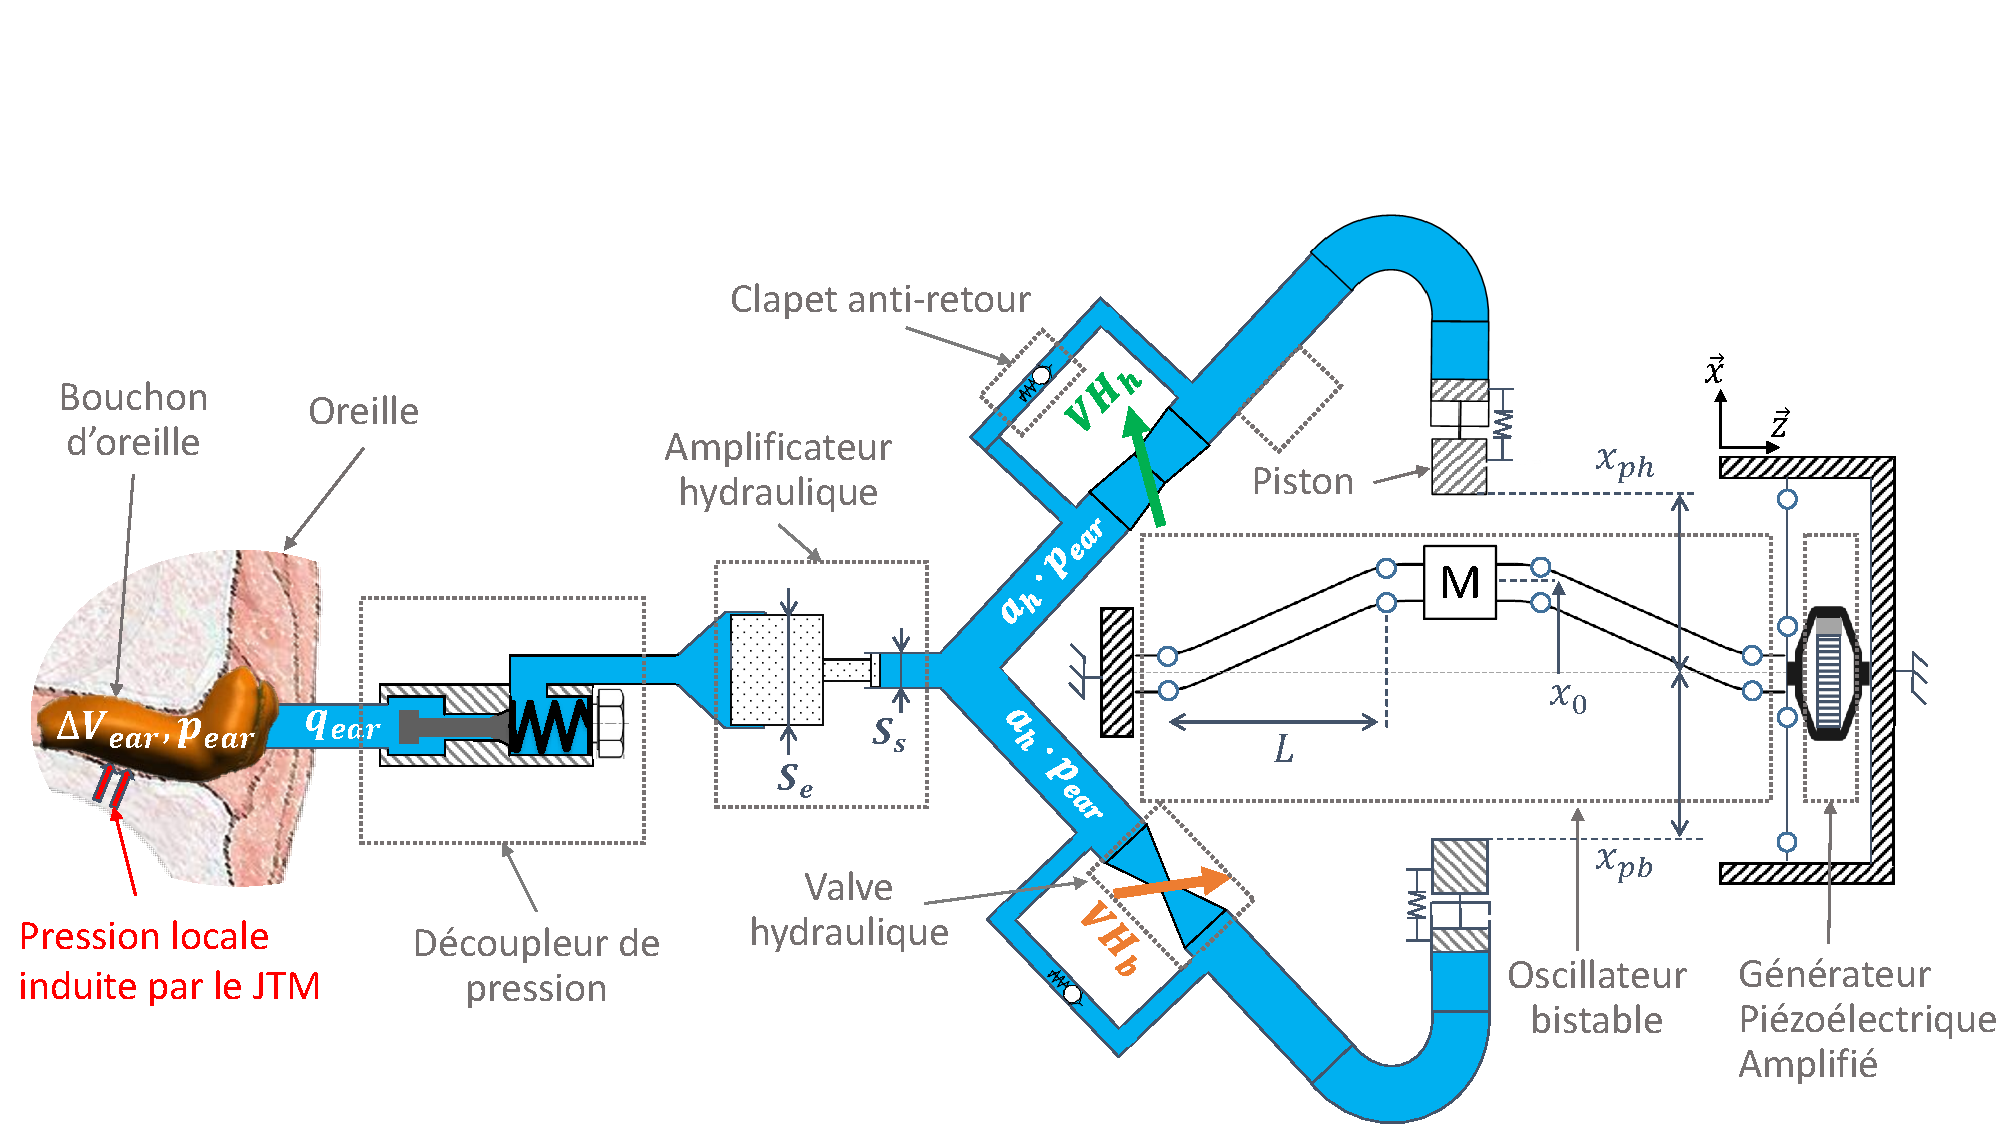
\includegraphics[trim={0cm 0cm 0cm 3.5cm},clip, width=\textwidth]{../Chap2/Figure/schema_systeme_complet_decoupleur.pdf}
		\caption{Schéma du système de récupération d'énergie proposé}
		\label{fig:schema_systeme_complet}
	\end{center}
\end{figure}
%%%%%%%%%%%%%%%%%%%%%%%

La mini pompe est remplie d'un fluide incompressible et reliée à deux PHs, \emph{haut} et \emph{bas}, au travers de deux valves hydrauliques (VH), respectivement VH$_h$ et VH$_b$, et, deux clapets anti-retour. Les pistons actionnent tour à tour l'OB et le GPA convertit ensuite en énergie électrique les oscillations de la masse dynamique de l'OB, symbolisée par la lettre 'M' sur la figure \ref{fig:schema_systeme_complet}. 

Le rôle de l'AH est d'adapter l'impédance hydraulique de la pompe, à l'impédance mécanique de l'OB. Cet étage d'amplification permettra d'adapter la pression de fonctionnement des pistons à la pression maximale admissible dans l'oreille. En effet, il faudra respecter le seuil de confort noté $p_c$, au-delà duquel le port du bouchon d'oreille deviendra désagréable pour l'utilisateur. Ceci est un critère de dimensionnement principal qui sera développé dans la section \ref{subsec:2.5.3:Simulation et resultats}. En effet, la pression d'entrée de l'amplificateur sera plus faible qu'en sortie et inversement quant aux volumes balayés. Le rapport des pressions et volumes est directement donné par la géométrie de l'AH avec le rapport des sections comme suit :
\begin{equation}
	p_s = p_e \biggl( \frac{S_e}{S_s} \biggl)
	~~~~et~~~~
	\Delta V_s = \Delta V_e \biggl( \frac{S_s}{S_e} \biggr)
\end{equation}
Où $S$, $P$ et $\Delta V$ sont respectivement la surface rencontrée par le fluide, le volume balayé et la pression du fluide. L'indice "e" se réfère aux grandeurs en entrée de l'amplificateur et l'indice "s" aux grandeurs en sortie. On définit alors le rapport d'amplification hydraulique $a_h$ tel que
\begin{equation}
	a_h = \frac{S_e}{S_s}
\end{equation}
On a alors 
\begin{equation}
	p_s =  a_h\ p_e 
	~~~~et~~~~
	\Delta V_s = \dfrac{\Delta V_e}{a_h}
	\label{eq:volume_sortant_aplificateur_hydraulique}
\end{equation}

D'autre part, le bouchon d'oreille doit être gonflé à une pression suffisante afin que sa paroi épouse bien celle de l'oreille, pour un transfert mécanique optimal.

L'étage de découplage de pression permettra de gonfler le bouchon d'oreille sans que les pistons ne se retrouvent en butée à cause de l'effet de la pression de gonflage $p_{gon}$. Le découpleur de pression doit être réglé de façon à laisser passer le débit seulement si la mâchoire est en mouvement, en filtrant de ce fait la pression statique de gonflage. $\Delta p_{ear}$ définit alors la variation de pression induite par la mastication. La pression totale $p_{ear}$ dans l'oreille peut donc être calculée par l'équation \ref{eq: variation de pression DeltaP_ear}.
\begin{equation}
	 p_{ear} = \Delta p_{ear} +  p_{gon}
	 \label{eq: variation de pression DeltaP_ear}
\end{equation}

Le découpleur agit de la même manière qu'un clapet anti-retour réglable. Une publication de 2020 recense plusieurs études sur le développement et la miniaturisation de ce type de composants pour des faibles pressions de fonctionnement. Visant principalement une utilisation médicale pour le dosage de médicaments, les dispositifs existants sont capables d'atteindre l'échelle micrométrique, avec des pressions de réglage allant du kilopascal à quelques dizaines de kilopascals \cite{Wang2020}. Tout en sachant que des solutions existent pour le découplage hydraulique à faibles pressions de fonctionnement (<10kPa), cet aspect du récupérateur ne sera pas développé dans ces travaux de thèse.

Il est important d'identifier à présent les contraintes technologiques et celles du contexte applicatif liées à la méthode de conversion choisie, ainsi qu'à l'architecture générale du récupérateur. On identifie une contrainte de contexte applicatif et plusieurs contraintes technologiques principales.
\begin{itemize}[label=$\blacksquare$]
\item \emph{Contraintes de contexte applicatif :} Même si le dispositif est à l'extérieur de l'oreille, l'échelle des éléments doit rester en adéquation avec la taille d'un boiter d'appareil d'aide à l'audition standard, dont le volume peut être approximé par un pavé de dimensions 50x20x10mm$^3$.
\item \emph{Contraintes technologiques :}
	\begin{itemize}[label=$\circ$]
		\item La pression $p_{ear}$ du bouchon d'oreille est de quelques dizaines de millibars. Les PHs doivent donc admettre des pressions de fonctionnement faibles afin qu'il soit possible de les mettre en mouvement, mais aussi, pour réduire les frottements secs dans le joint d'étanchéité du piston. Un compromis est donc à trouver entre le niveau d'étanchéité et les pertes par frottements du piston.
		\item Les VHs de doivent pas, en positions ouverte, générer trop de pertes de charges. Les dimensions de la technologie répondant au besoin doivent être cohérentes avec celles du contexte applicatif discuté précédemment.
		\item L'implémentation directe de céramiques PZT sur une structure oscillante bistable nécessite d'adapter l'impédance mécanique de l'oscillateur avec celle des céramiques. En effet, ces dernières pourront absorber des contraintes importantes, mais leur rupture fragile (sans déformation plastique) les limite fortement en déplacement. L'utilisation d'un amplificateur/réducteur de contraintes/déplacements, appelé aussi flextenseur dans la littérature, permet de remédier à ce problème \cite{Snyder2007,Guo2019,Aldrich1994,Zhou2013}. Le paragraphe qui suit décrit plus en détails les avantages apportés par une telle structure.
	\end{itemize}
\end{itemize}
		%*************
		\subsubsection{Le principe du flextenseur}
		\label{subsec:2.1.2.a_Le principe du flextenseur}
		%*************
%%%%%%%%%%%%%%%%%%%%%%%%%%
\begin{figure}[!htbp]
	\begin{center}
		\begin{subfigure}[b]{0.45\textwidth}
			\captionsetup{justification=centering}
			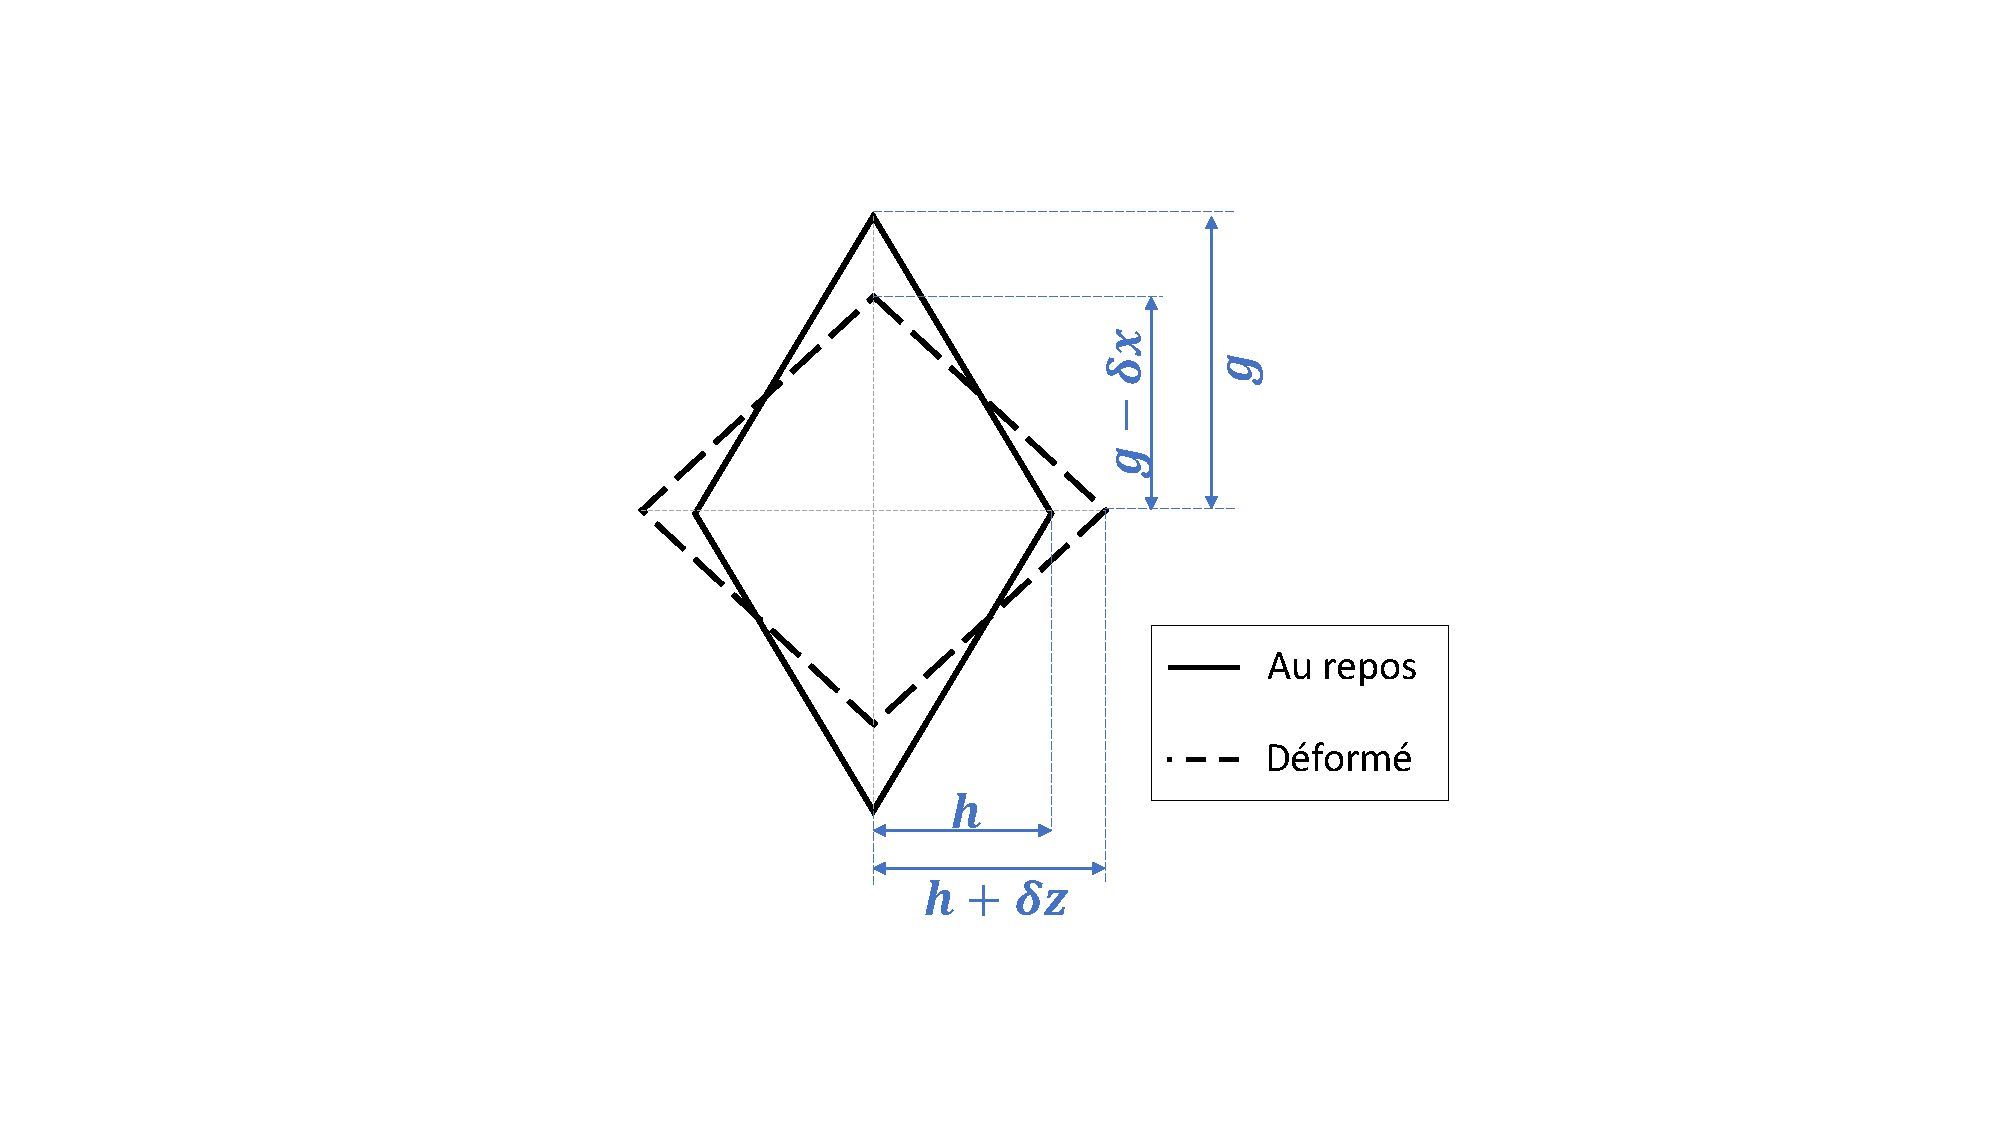
\includegraphics[trim={10.5cm 1cm 9cm 3cm},clip,width=\textwidth]{../Chap2/Figure/flextenseur_cinematique.pdf}
			\caption{ Comportement cinématique}
			\label{fig:flextenseur_cinématique}
		\end{subfigure}
		\begin{subfigure}[b]{0.45\textwidth}
			\captionsetup{justification=centering}
			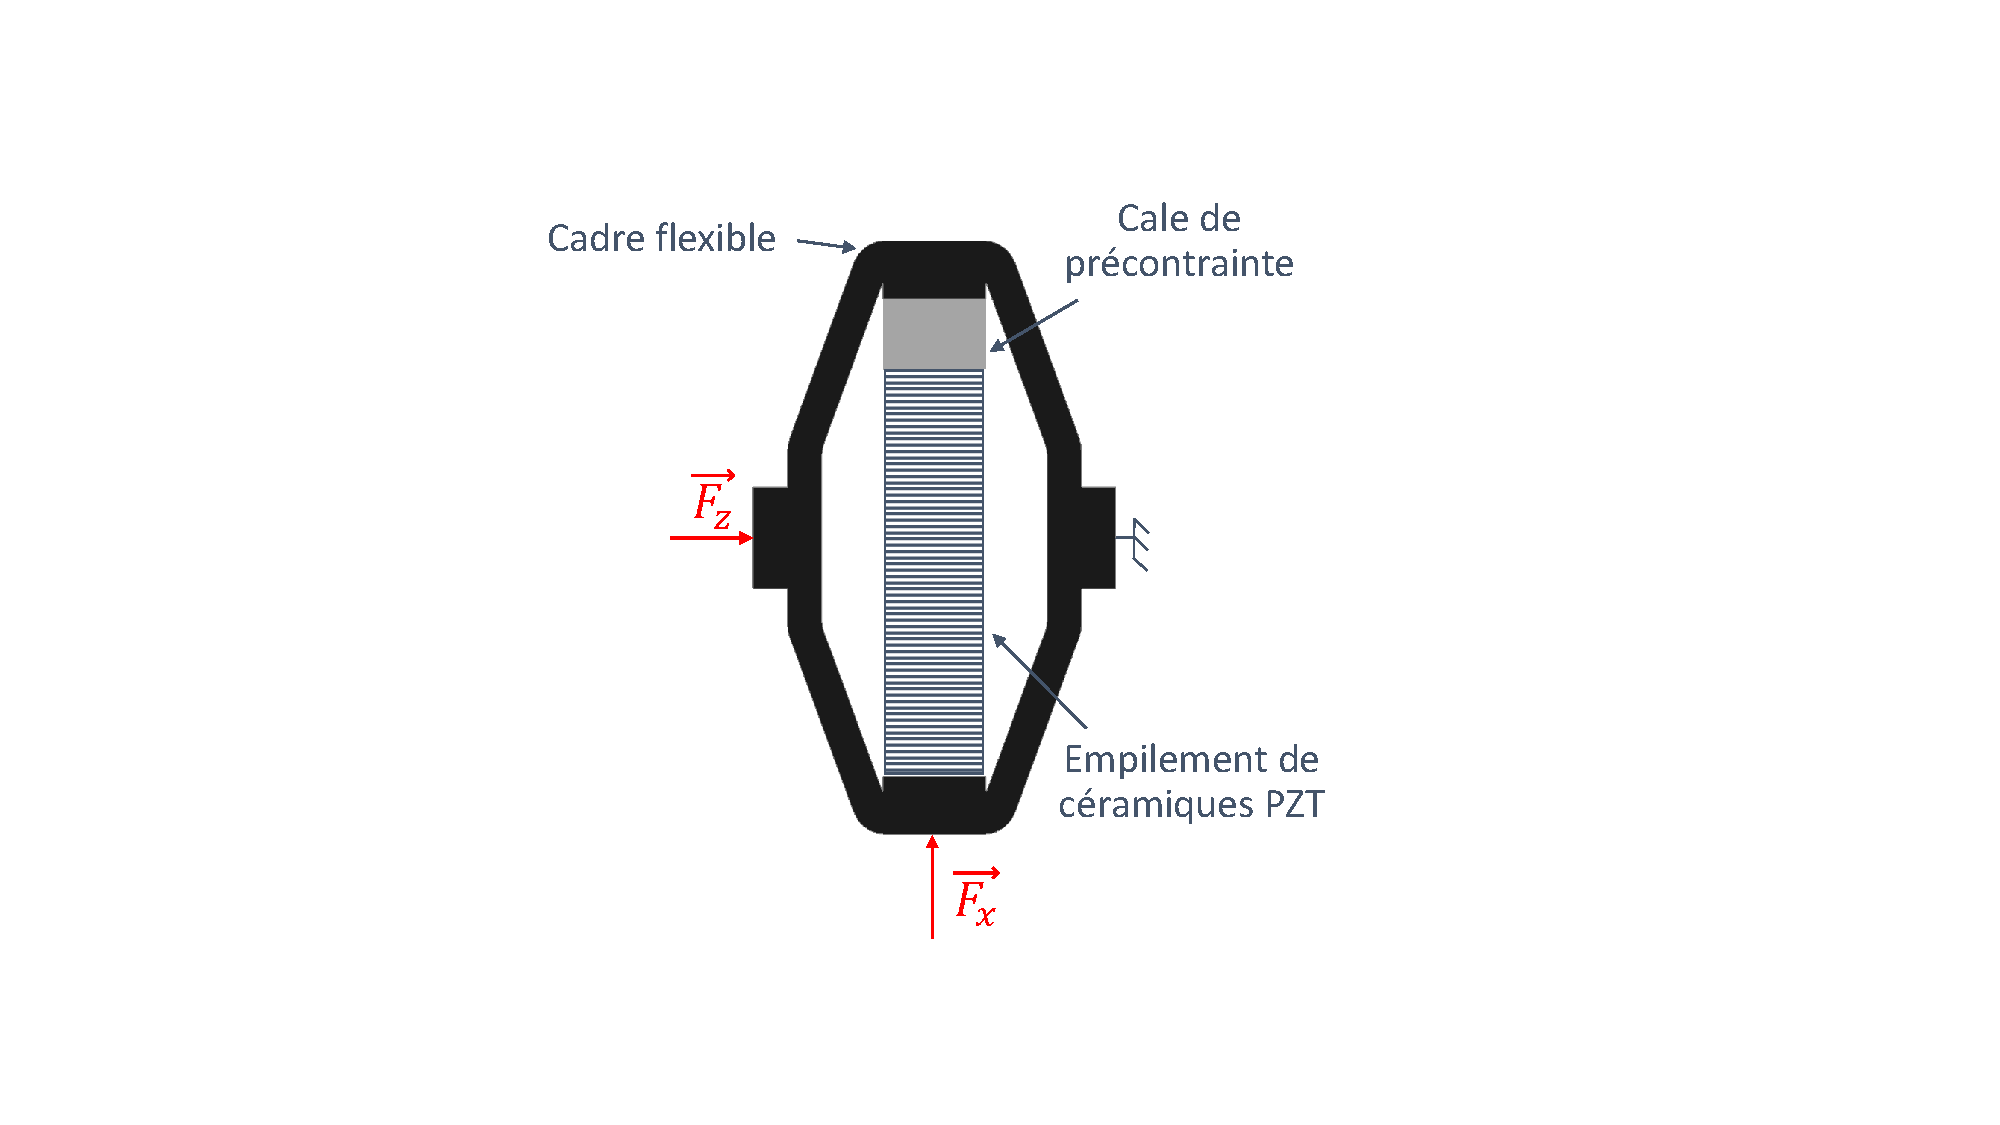
\includegraphics[trim={9cm 3cm 11.5cm 3cm},clip,width=\textwidth]{../Chap2/Figure/flextenseur_statique.pdf}
			\label{fig:flextenseur_statique}
			\caption{Comportement statique}
		\end{subfigure}
		\caption{Comportement du flextenseur \cite{Zhou2013}}
		\label{fig:flextenseur}
	\end{center}
\end{figure}
%%%%%%%%%%%%%%%%
Le flextenseur mécanique convertit un déplacement important sur l'axe $\vec{z}$ du transducteur en un déplacement plus faible sur l'axe $\vec{x}$. À l'inverse, les contraintes suivant l'axe $\vec{x}$ sont augmentées par rapport à celles sur l'axe $\vec{z}$. La figure \ref{fig:flextenseur} et les équations \ref{eq_flextenseur_cinématique} et  \ref{eq_flextenseur_statique} décrivent le comportement statique et cinématique des structures en flextension.

Notons par ailleurs que les céramiques sont sollicitées en traction/compression. De ce fait, le coefficient de couplage électromécanique pour la conversion d'énergie fait intervenir le mode de sollicitation longitudinal du matériau piézoélectrique, aussi appelé mode 33. Il est en effet celui à privilégier, devant les autres modes de déformation, pour maximiser le rendement de conversion des céramiques piézoélectriques \cite{OmegaPiezo2022,Zhang2018,Fujishima1984}.
%%%%%%%%%%%%%%%%%%%%%%
\begin{equation}
	\delta x = \biggl( \frac{h}{g} \biggr) \delta z
\label{eq_flextenseur_cinématique}
\end{equation}
%%%%%%%%%%%%%%%
\begin{equation}
	\vec{F_x} = \biggl(  \frac{g}{h} \biggr) \vec{F_z}
\label{eq_flextenseur_statique}
\end{equation}
%%%%%%%%%%%%%%
	%*************
	\subsubsection{Description du fonctionnement des PHs, VHs, OB et GPA}
	\label{subsec:2.1.2.b_Description du fonctionnement du système}
	%*************
Pour comprendre le couplage dynamique entre les principaux organes, le comportement du système en concordance avec les mouvements de la mâchoire est décrit et illustré dans le tableau \ref{tbl:act_top}. On suppose que M se trouve à la position d'équilibre supérieure en $x=x_0$ à l'étape 1 et que la mâchoire est en position ouverte. 

Un cycle de mastication comprenant une ouverture de mâchoire, suivie d'une fermeture de mâchoire, permet de faire franchir à M le seuil de potentiel élastique en $x=0$ une seule fois. Lorsque cela se produit deux fois et que la masse est revenue à sa position initiale, elle a complété un cycle. Deux cycles de mastication sont donc nécessaires afin de compléter un cycle de fonctionnement complet du point de vue du récupérateur. Par ailleurs, l'énergie hydraulique QS est transmise à l'OB à la fréquence de mastication $f_{ear}=1,57$Hz. Elle est ensuite convertie en énergie oscillatoire, dont la fréquence $f_0$ est supérieure à $f_{ear}$ et sera définie par la suite avec les différents paramètres de l'OB.
%%%%%%%%%%%%%%%%%%%%%%%%%%%%%%%%%%%%%%%%%%%
\newpage
\begin{table}[!htbp]
\centering
%\rowcolors[]{2}{black!8}{}{
\renewcommand{\arraystretch}{2}
\begin{tabular}{c m{9cm}}
\rowcolor{blue!10}
%\cmidrule[1pt]{1-5}
\toprule
\multicolumn{1}{c}{\textbf{Étape}} & \multicolumn{1}{c}{\textbf{\emph{Conditions initiales} et description}} \\
\midrule
%%%%%%%%%%%%% PHASE 1 %%%%%%%%%%%%%%%%%%%
\raisebox{-.5\height}{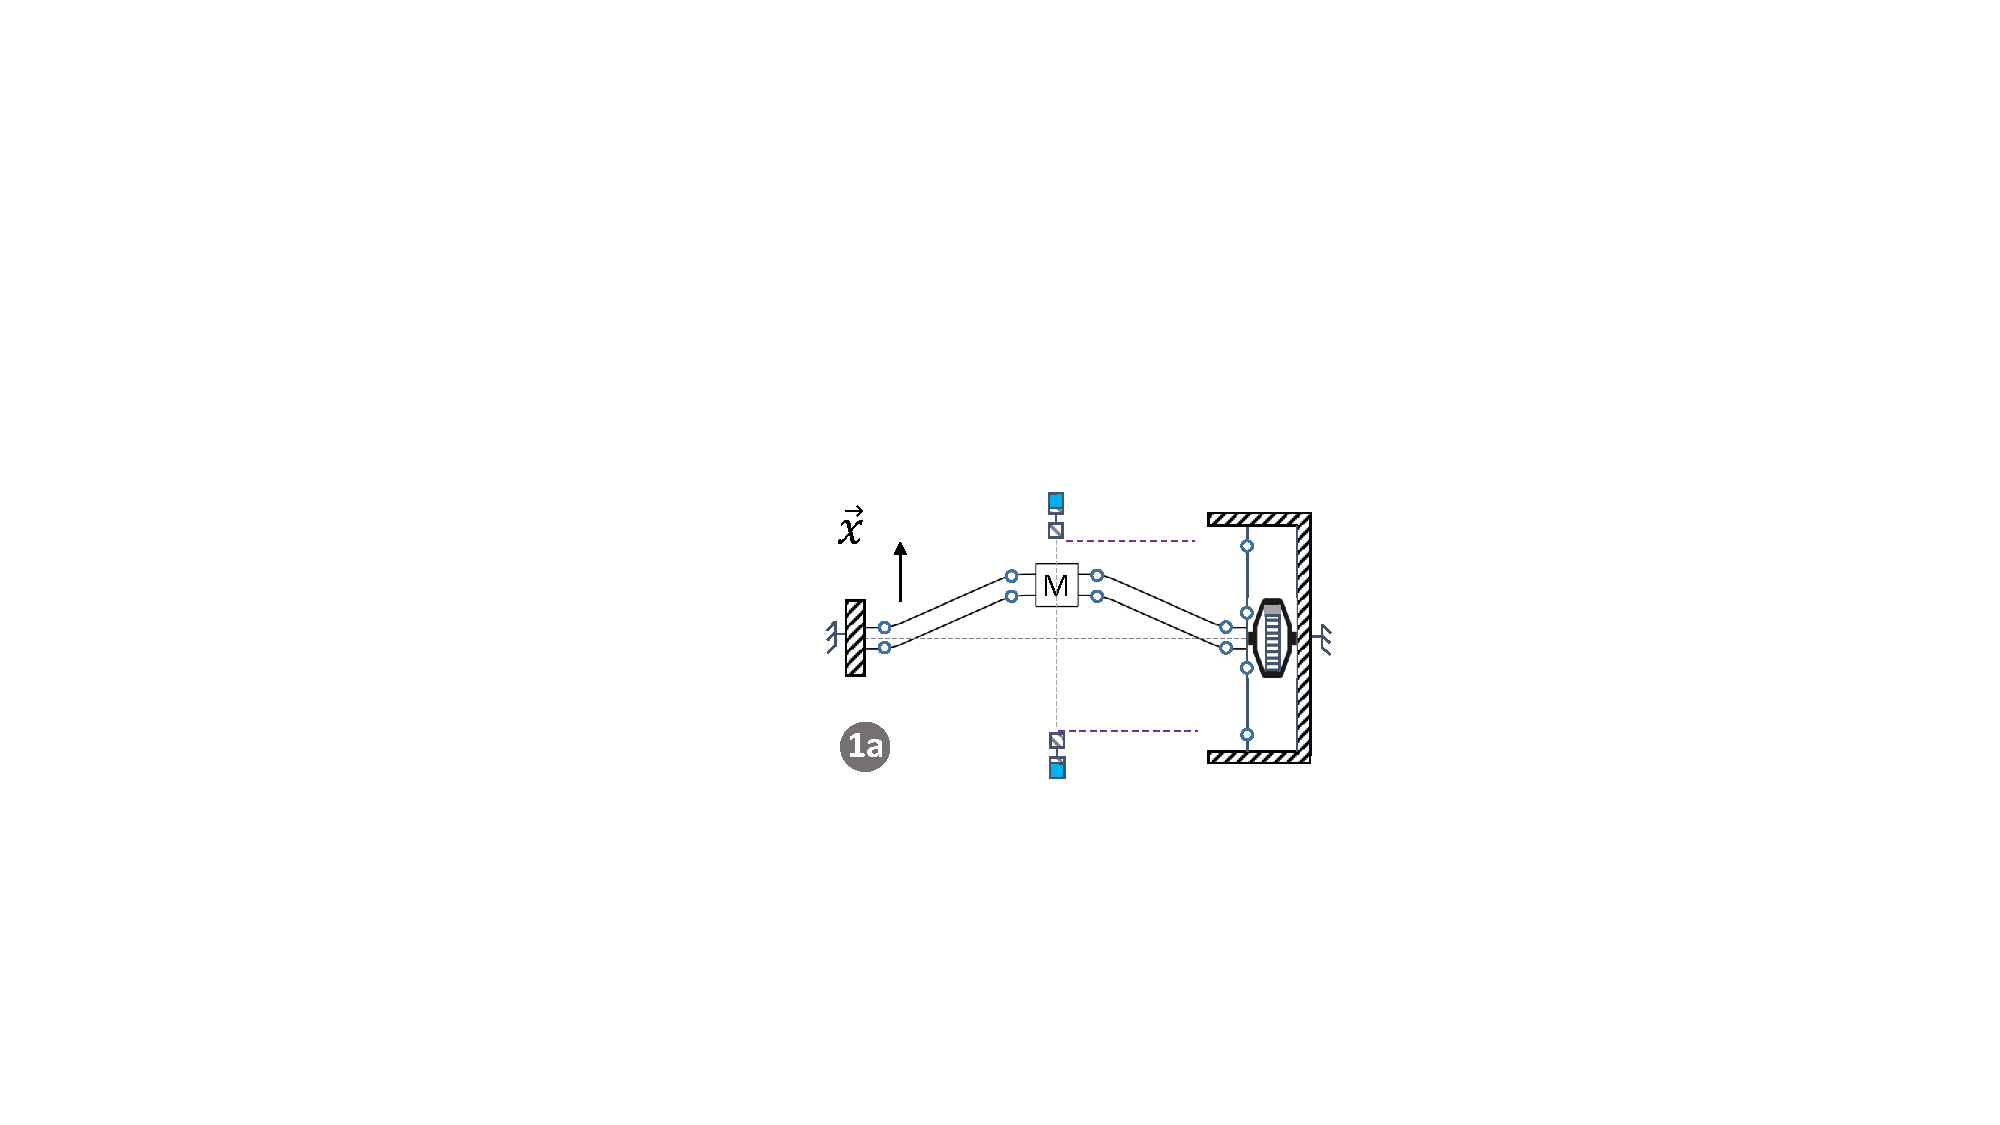
\includegraphics[trim={13.5cm 5.5cm 11cm 8cm},clip,width=5cm]{../Chap2/Figure/phases_act/phase_act_1.pdf}}
& \emph{Mâchoire ouverte, VH$_h$ fermée, VH$_b$ ouverte} \newline
Les pistons sont en position de retrait et M est à l'équilibre en $x_0$. Il n'y a pas de contact entre M et les pistons. \\ 
\hline
\hline 
%%%%%%%%%%%%%%% PHASE 2 %%%%%%%%%%%%%%%%%%%
\raisebox{-.5\height}{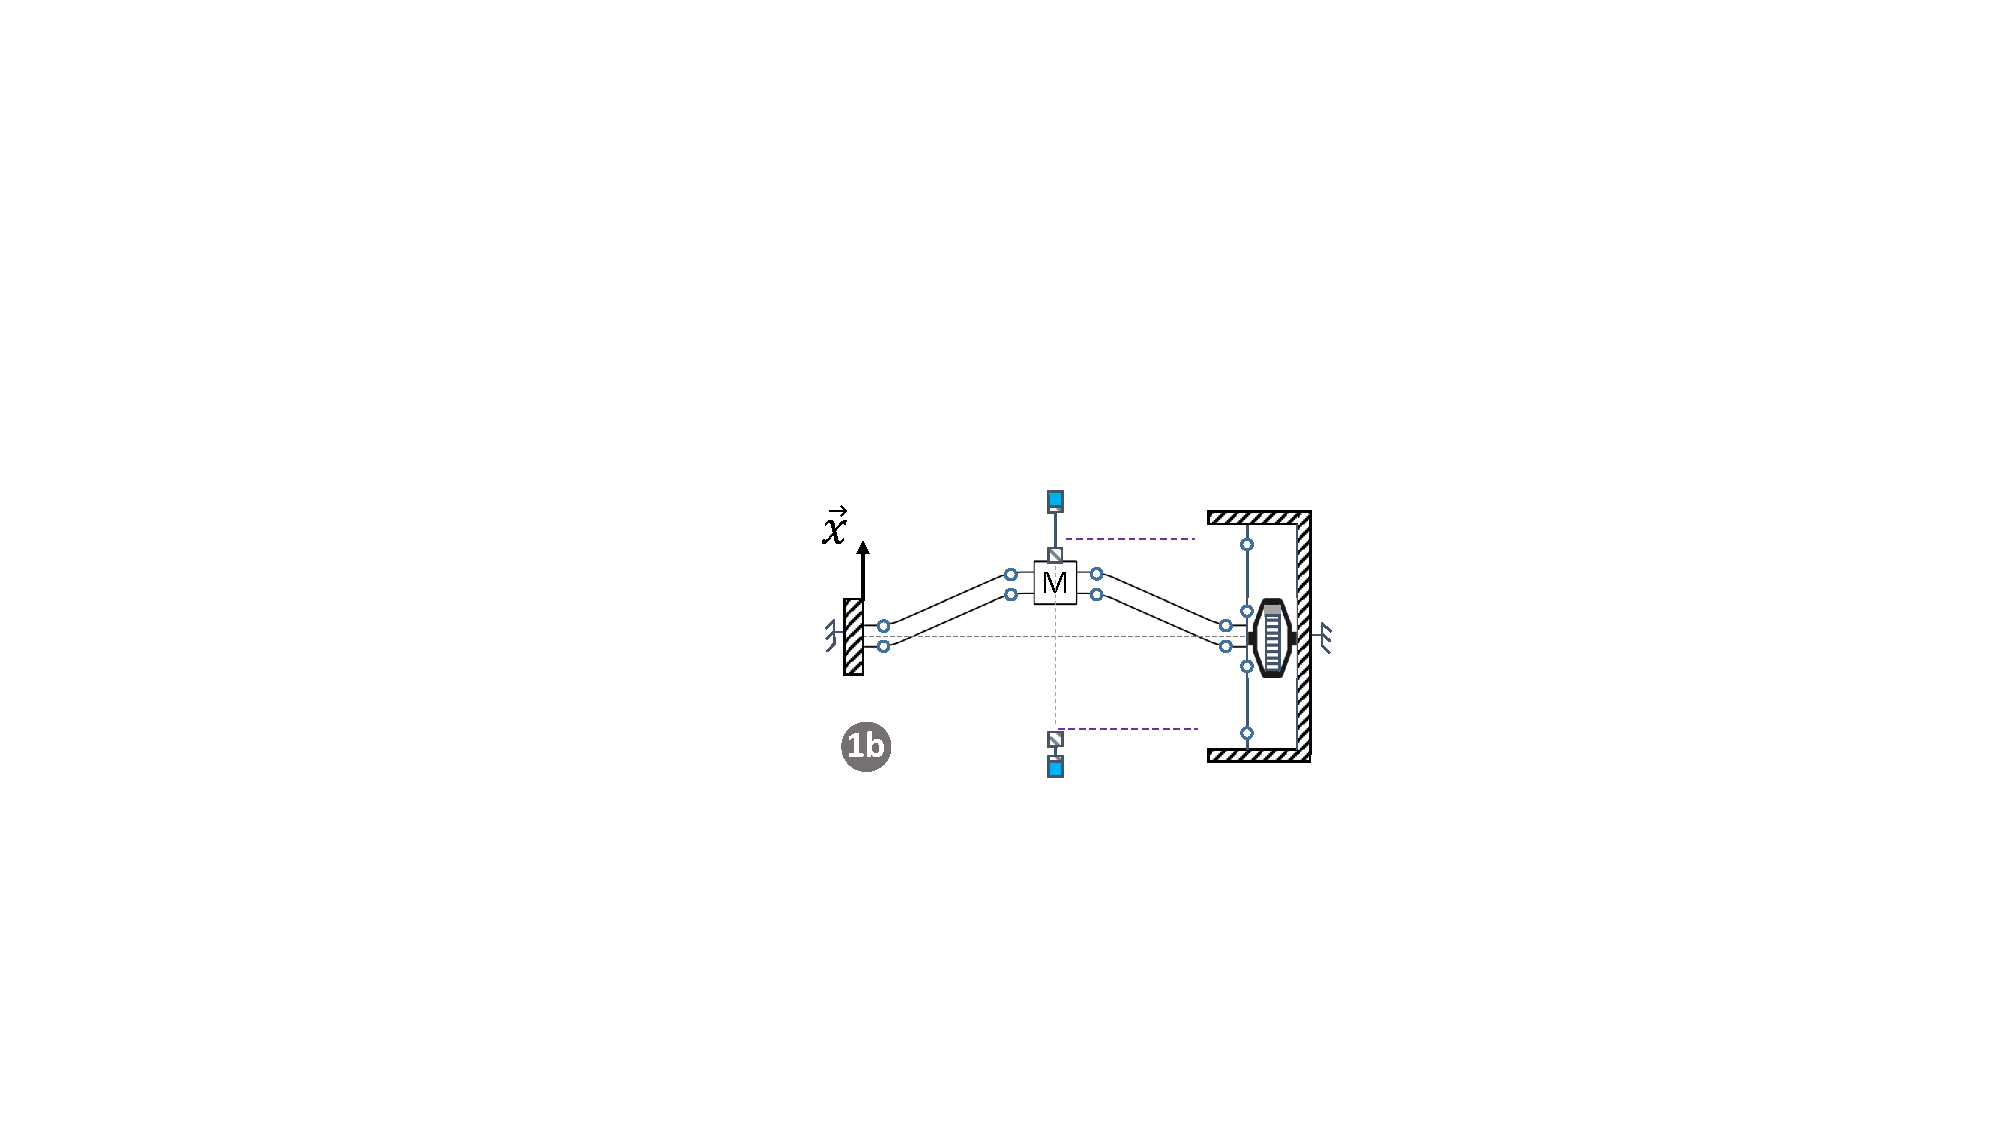
\includegraphics[trim={13.5cm 5.8cm 11cm 8.1cm},clip,width=5cm]{../Chap2/Figure/phases_act/phase_act_2.pdf}}
&  \emph{Mâchoire en cours de fermeture, VH$_h$ fermée, VH$_b$ ouverte}.
\newline Le fluide sortant du bouchon d'oreille actionne le piston haut en direction de M. La masse est poussée en régime QS vers sa position d'équilibre instable en $x=0$. \\ 
\hline
\hline
%%%%%%%%%%%%%%% PHASE 3 %%%%%%%%%%%%%%%%%%%
\raisebox{-.5\height}{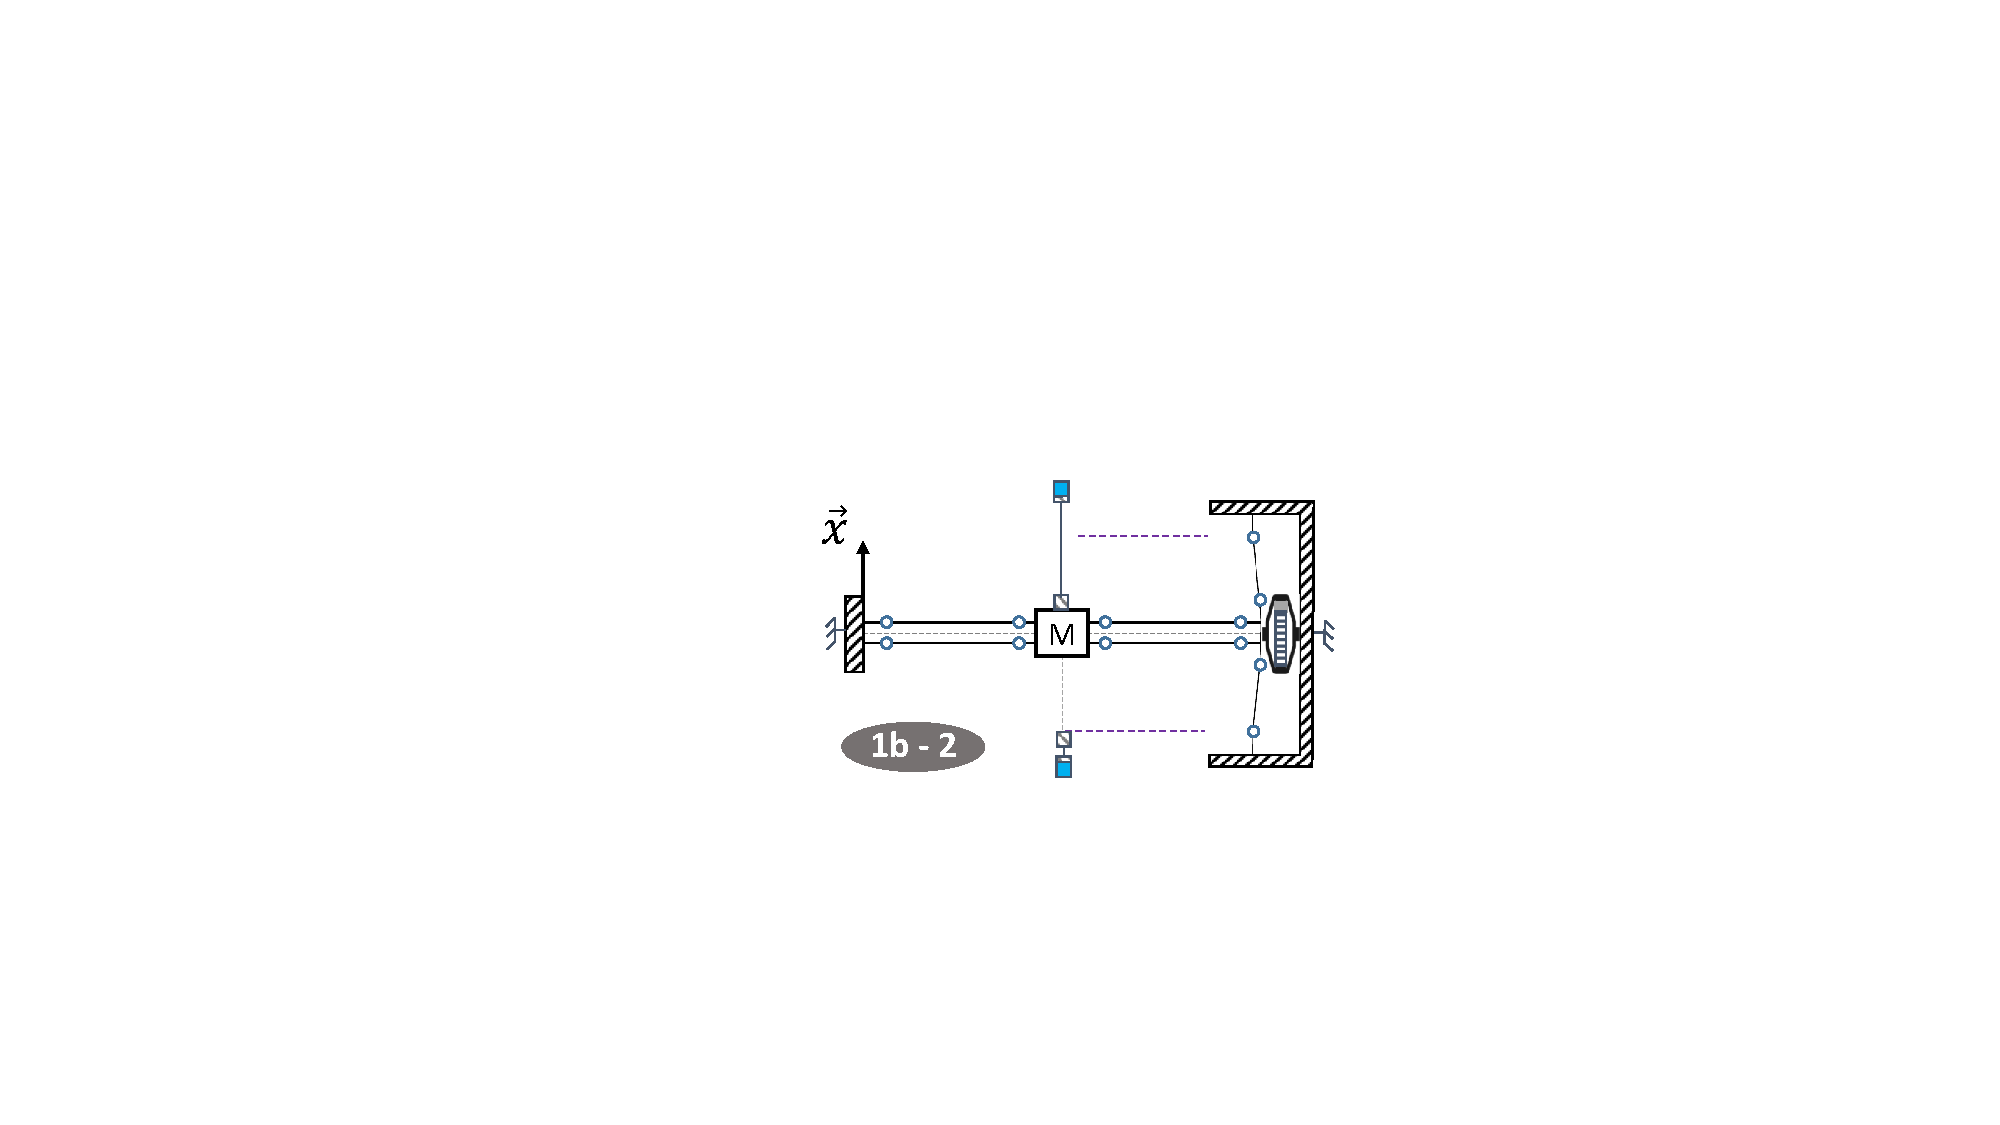
\includegraphics[trim={13.5cm 5.8cm 11cm 8.1cm},clip,width=5cm]{../Chap2/Figure/phases_act/phase_act_3.pdf}}
& \emph{Mâchoire fermée, VH$_h$ et VH$_b$ ouvertes}.
\newline La symétrie du système impose l'ouverture simultanée des deux $VH$ pendant un court instant, lorsque la masse dynamique traverse sa position d'équilibre instable en $x=0$ pour basculer vers l'équilibre opposé en $x=-x_0$.\\ 
\hline
\hline
%%%%%%%%%%%%%%% PHASE 4 %%%%%%%%%%%%%%%%%%%
\raisebox{-.5\height}{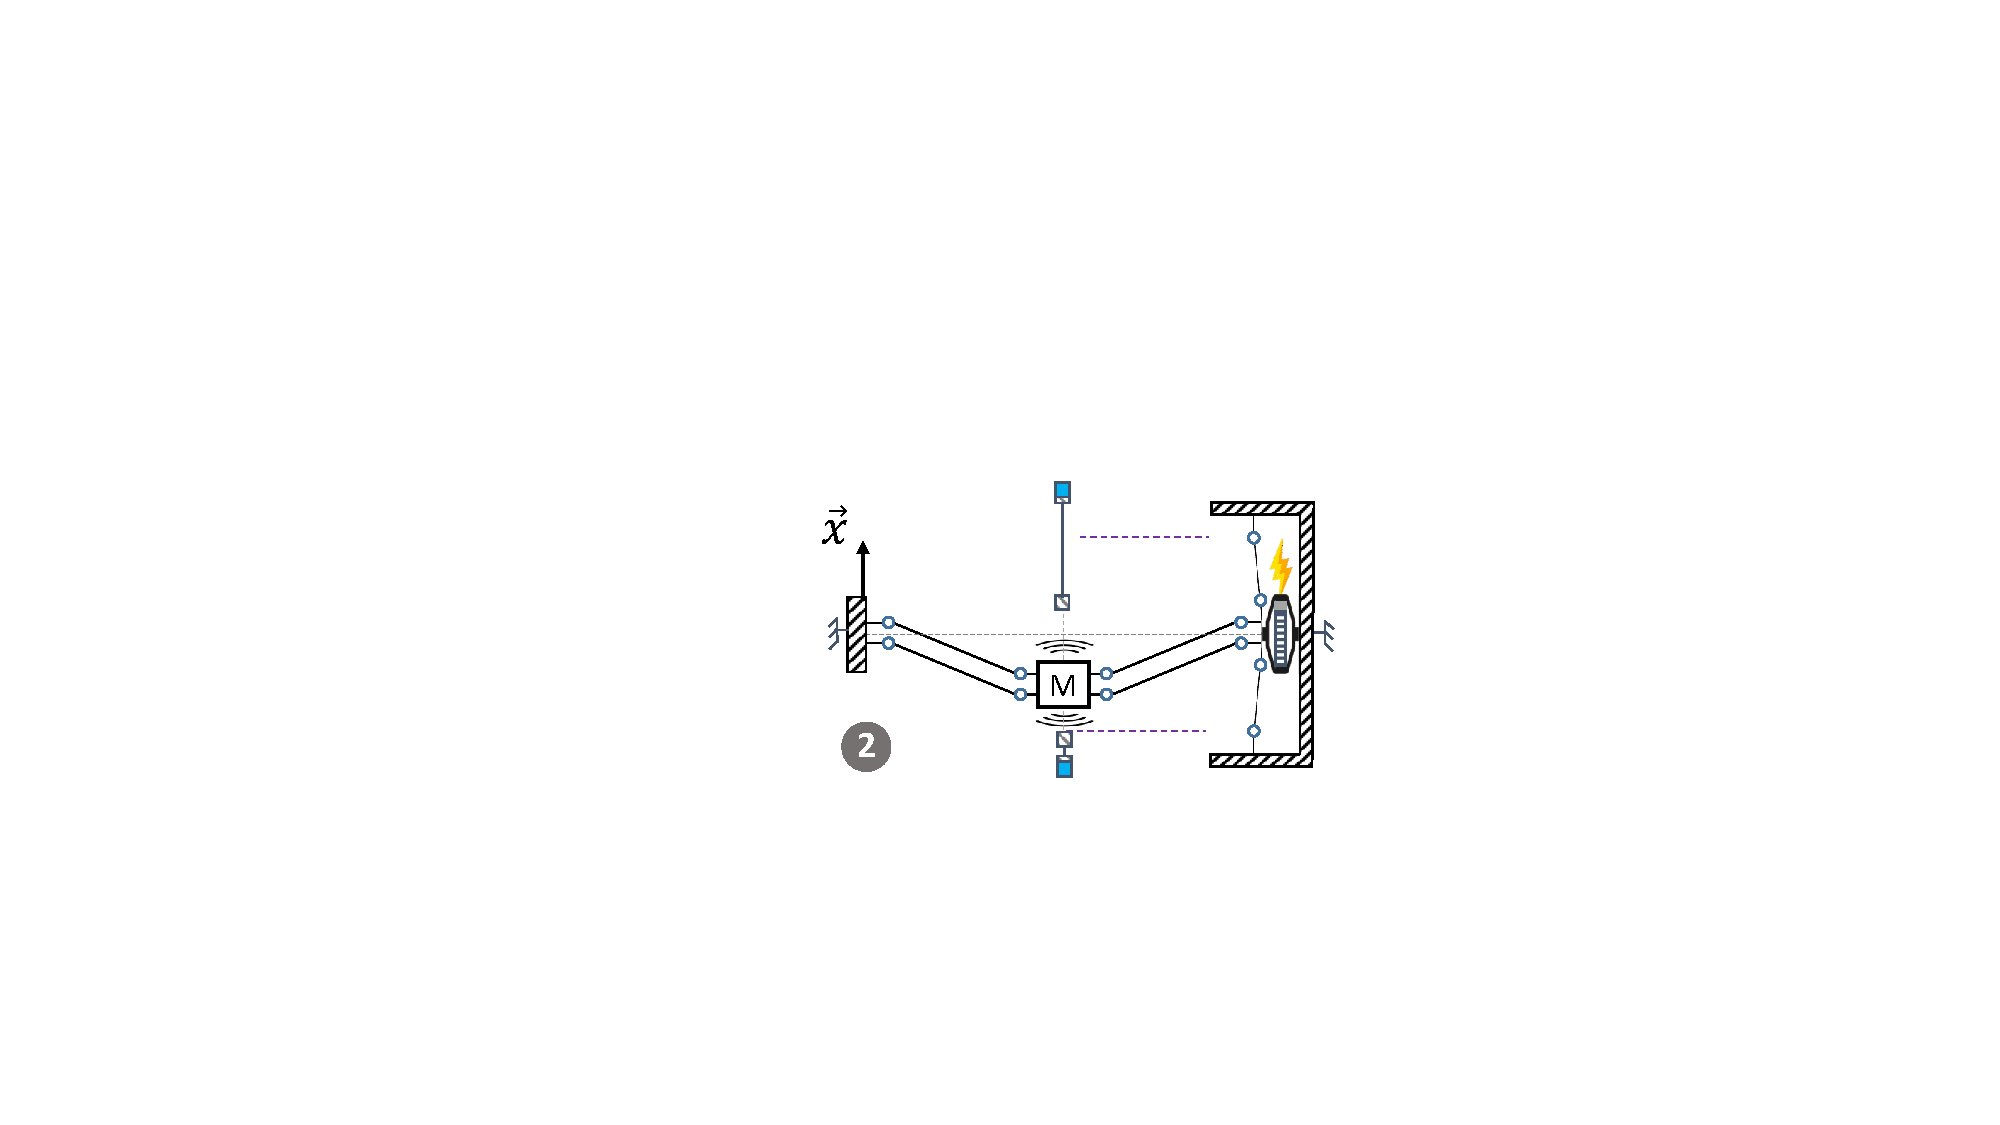
\includegraphics[trim={13.5cm 5.8cm 11cm 8.2cm},clip,width=5cm]{../Chap2/Figure/phases_act/phase_act_4.pdf}}
& \emph{Mâchoire fermée, VH$_h$ fermée, VH$_b$ ouverte}. 
\newline La valve VH$_b$ s'ouvre, mais le piston bas ne bouge pas, car le volume sortant du bouchon d'oreille a été déplacé dans le piston haut lors de la poussée. M bascule alors vers le puits de potentiel bas en $x=-x_0$ et oscille autour de celui-ci à une fréquence 30 fois supérieure à celle de mastication. Une partie substantielle (définie par le coefficient de couplage du système) de l'énergie d'oscillation est alors convertie en électricité par le biais du GPA, jusqu'à l'arrêt complet des oscillations. \\
\hline
\hline
%%%%%%%%%%%%% PHASE 5 %%%%%%%%%%%%%%%%%%%
\raisebox{-.5\height}{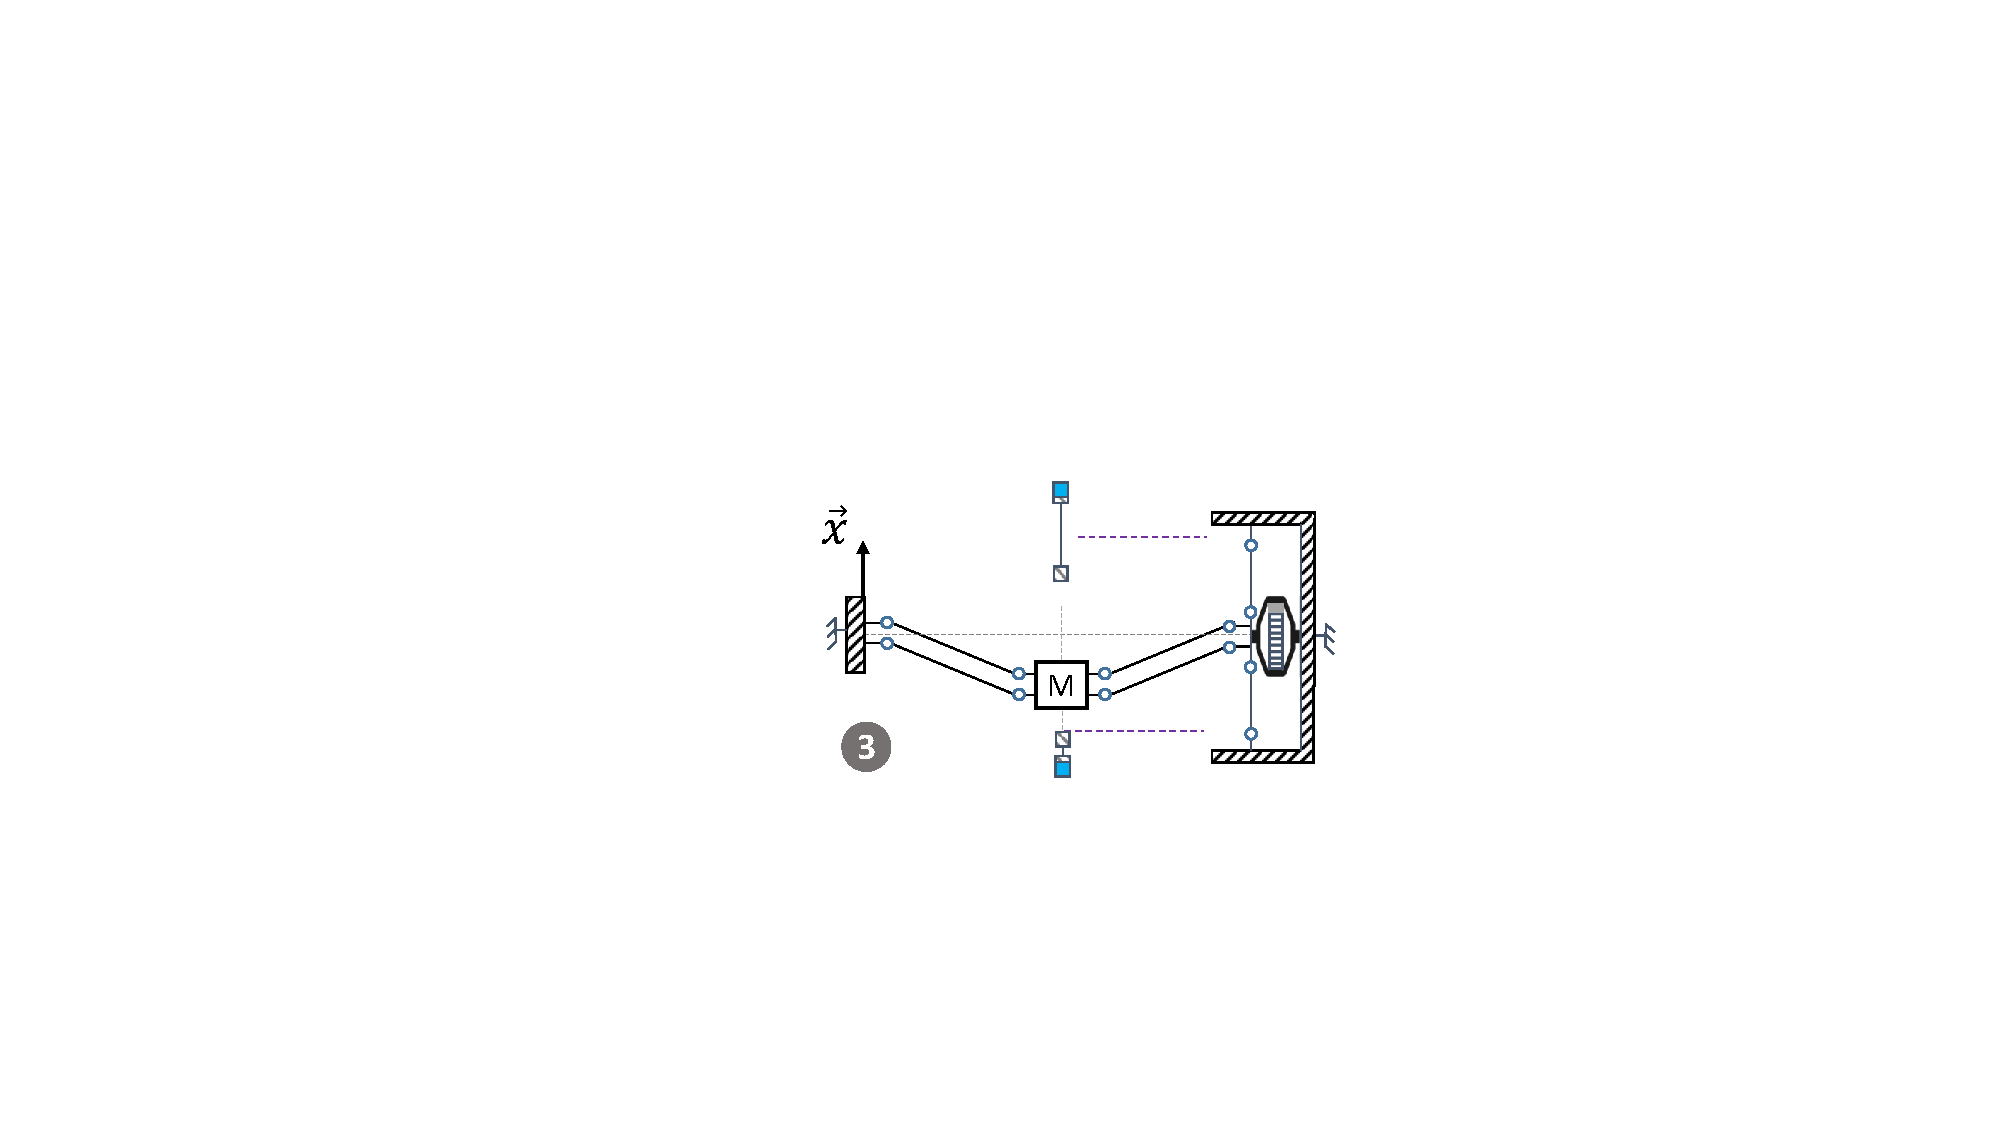
\includegraphics[trim={13.5cm 5.8cm 11cm 8.1cm},clip,width=5cm]{../Chap2/Figure/phases_act/phase_act_5.pdf}}
&  \emph{Mâchoire en cours d'ouverture, VH$_h$ fermée, VH$_b$ ouverte}.
\newline M est quasiment à l'arrêt en $x=-x_0$. L'ouverture de la bouche crée une dépression relative à la pression de gonflage ($p_{ear}<p_{gon}$) et, par conséquent, le piston haut recule vers sa position de base avant actionnement. \\ 
\hline
\hline
%%%%%%%%%%%%% PHASE 6 %%%%%%%%%%%%%%%%%%%
\raisebox{-.5\height}{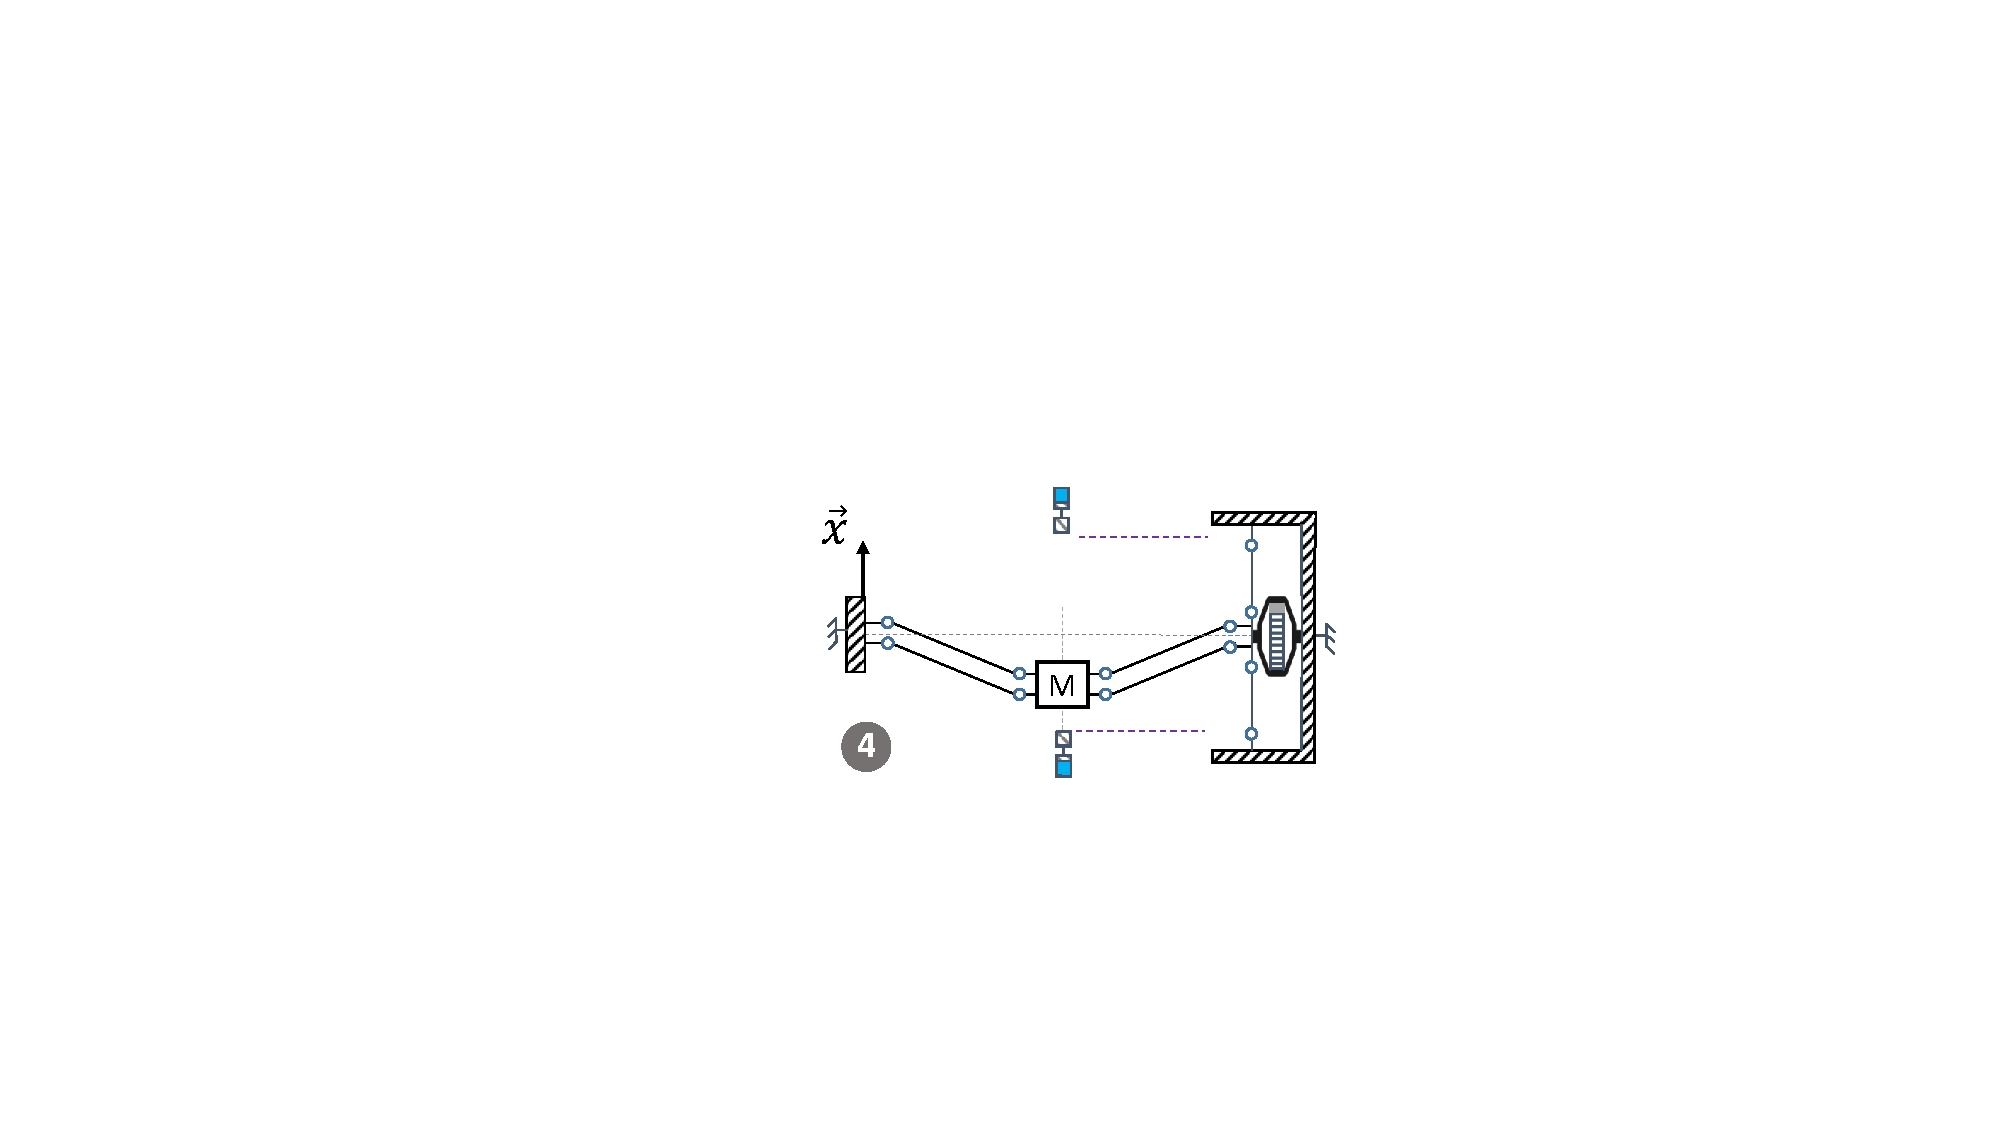
\includegraphics[trim={13.5cm 5.8cm 11cm 8.1cm},clip,width=5cm]{../Chap2/Figure/phases_act/phase_act_6.pdf}}
& \emph{Mâchoire ouverte, VH$_h$ fermée, VH$_b$ ouverte}. 
\newline On se retrouve dans des conditions symétriques à celles de la phase 1. Le prochain cycle de mastication se déroulera donc de la même façon par la poussée de M vers la position d'équilibre haute. Deux cycles de mastication compléteront donc un cycle complet du point de vue du système.\\ 
\bottomrule
%\cmidrule[1pt]{1-5}
\end{tabular}
%}
\caption{Phases de fonctionnement du récupérateur pour un cycle de mastication}
\label{tbl:act_top}
\end{table} 
%%%%%%%%%%%%%%%%%%%%%%%%%%%%%%%%%%%%%%%%%%%
%/!\/!\/!\/!\/!\/!\/!\/!\/!\/!\/!\/!\/!\/!\/!\/!\/!\/!\/!\/!\/!\/!\/!\/!\%
\section{Cyclage du mouvement de la masse dynamique du bistable : valves hydrauliques}
\label{sec:2.2_Cyclage du mouvement de la masse dynamique du bistable : valves hydrauliques}
%/!\/!\/!\/!\/!\/!\/!\/!\/!\/!\/!\/!\/!\/!\/!\/!\/!\/!\/!\/!\/!\/!\/!\/!\%
	Pour assurer un mouvement cyclique du point de vue de M, il est nécessaire qu'à chaque cycle de mastication le fluide sortant du bouchon d'oreille se dirige alternativement vers chacun des deux PHs. Dans la suite nous exposons les solutions technologiques existantes et introduisons la solution proposée dans ces travaux.\\ 
	Avant toute chose, il est nécessaire de dresser le cahier des charges pour le fonctionnement des valves hydrauliques. Celui-ci se décompose en trois principaux critères :
\begin{itemize}
	\item \emph{Critère hydraulique} : Pour le bon fonctionnement du système, il est nécessaire que le débit sortant du bouchon d'oreille soit redirigé vers un seul des deux pistons. Les pertes de charges (PdC) générées par la valve hydraulique en position fermée doivent donc être suffisamment élevées devant celles générées par la valve en position ouverte pour permettre un écoulement préférentiel dans la branche ouverte.
	\item \emph{Critère énergétique} : L'énergie emmagasinée, ainsi que l'énergie dissipée dans le fonctionnement des valves hydrauliques doivent être faibles devant l'énergie fournie par la source afin de maximiser le rendement global du récupérateur d'énergie.
	\item \emph{Critère de cyclage} : Le fonctionnement dynamique des deux valves doit être couplé afin qu'un état fermé pour une valve corresponde à un état ouvert pour l'autre, pour un cycle de mâchoire donné. Les états doivent s'inverser à chaque cycle de fermeture mâchoire, afin de permettre l'actionnement de M dans les deux sens.
\end{itemize}
	%////////////////////////////////////////////
	\subsection{Solutions existantes pour la gestion directionnelle de fluide en mouvement}
	\label{subsec:2.2.2_Solutions existantes pour la gestion directionnelle de fluide en mouvement}
	%////////////////////////////////////////////
La solution technologique la plus utilisée est le distributeur hydraulique. La figure \ref{fig:distributeur_hyd_HYDRAC} expose le schéma mécanique d'un distributeur à commande électrique qui répondrait à notre besoin \cite{HYDRACINTERNATIONAL2022}. Le fonctionnement et les détails complets liés au dispositif sont présentés en annexe \ref{Ann:3 Fiche technique disctributeur Hydrac}. C'est un dispositif d'aiguillage hydraulique dont la plupart des types de commandes existantes sont électriques, hydrauliques ou pneumatiques. Notre système nous donne accès à une source hydraulique et une source électrique au travers de la récupération d'énergie. Cependant, au vu des faibles volumes de fluide déplacés dans le bouchon d'oreille (fig. \ref{fig:debit_ear}), il serait difficile de prévoir le pilotage hydraulique des distributeurs sans risquer de compromettre la course des pistons. La solution du pilotage électrique serait alors la plus simple à mettre en \oe{}uvre. Le schéma hydraulique de la figure \ref{fig:distributeur_hyd} montre la façon dont se ferait la redirection du débit entrant et sortant d'un distributeur hydraulique. Le bouchon d'oreille y est schématisé comme une pompe hydraulique à double sens de flux. Le distributeur hydraulique est, quant à lui, de type 3/2 (3 orifices et 2 positions). En effet, dans notre cas, nous avons deux directions souhaitées, alternativement vers le piston du haut, puis le piston du bas. Une commande électrique, faisant généralement déplacer le noyau d'un solénoïde, permet alors de présenter alternativement la chambre de distribution adéquate en sortie du bouchon d'oreille, afin d'alimenter un seul des deux pistons à la fois. La pompe étant à double sens de flux, la commutation pourrait se faire avec une butée de rentrée du piston qui vient de procéder à l'actionnement. Un tel système présente l'avantage d'une architecture simple et répond aisément au critère hydraulique du cahier des charges dressé précédemment. En revanche, la nécessité d'une commande électrique pour l'utilisation d'un tel dispositif impose d'investir une partie de l'énergie électrique récupérée afin de maintenir le cyclage du système. 
\begin{figure}
	\begin{center}
		\captionsetup{justification=centering}
		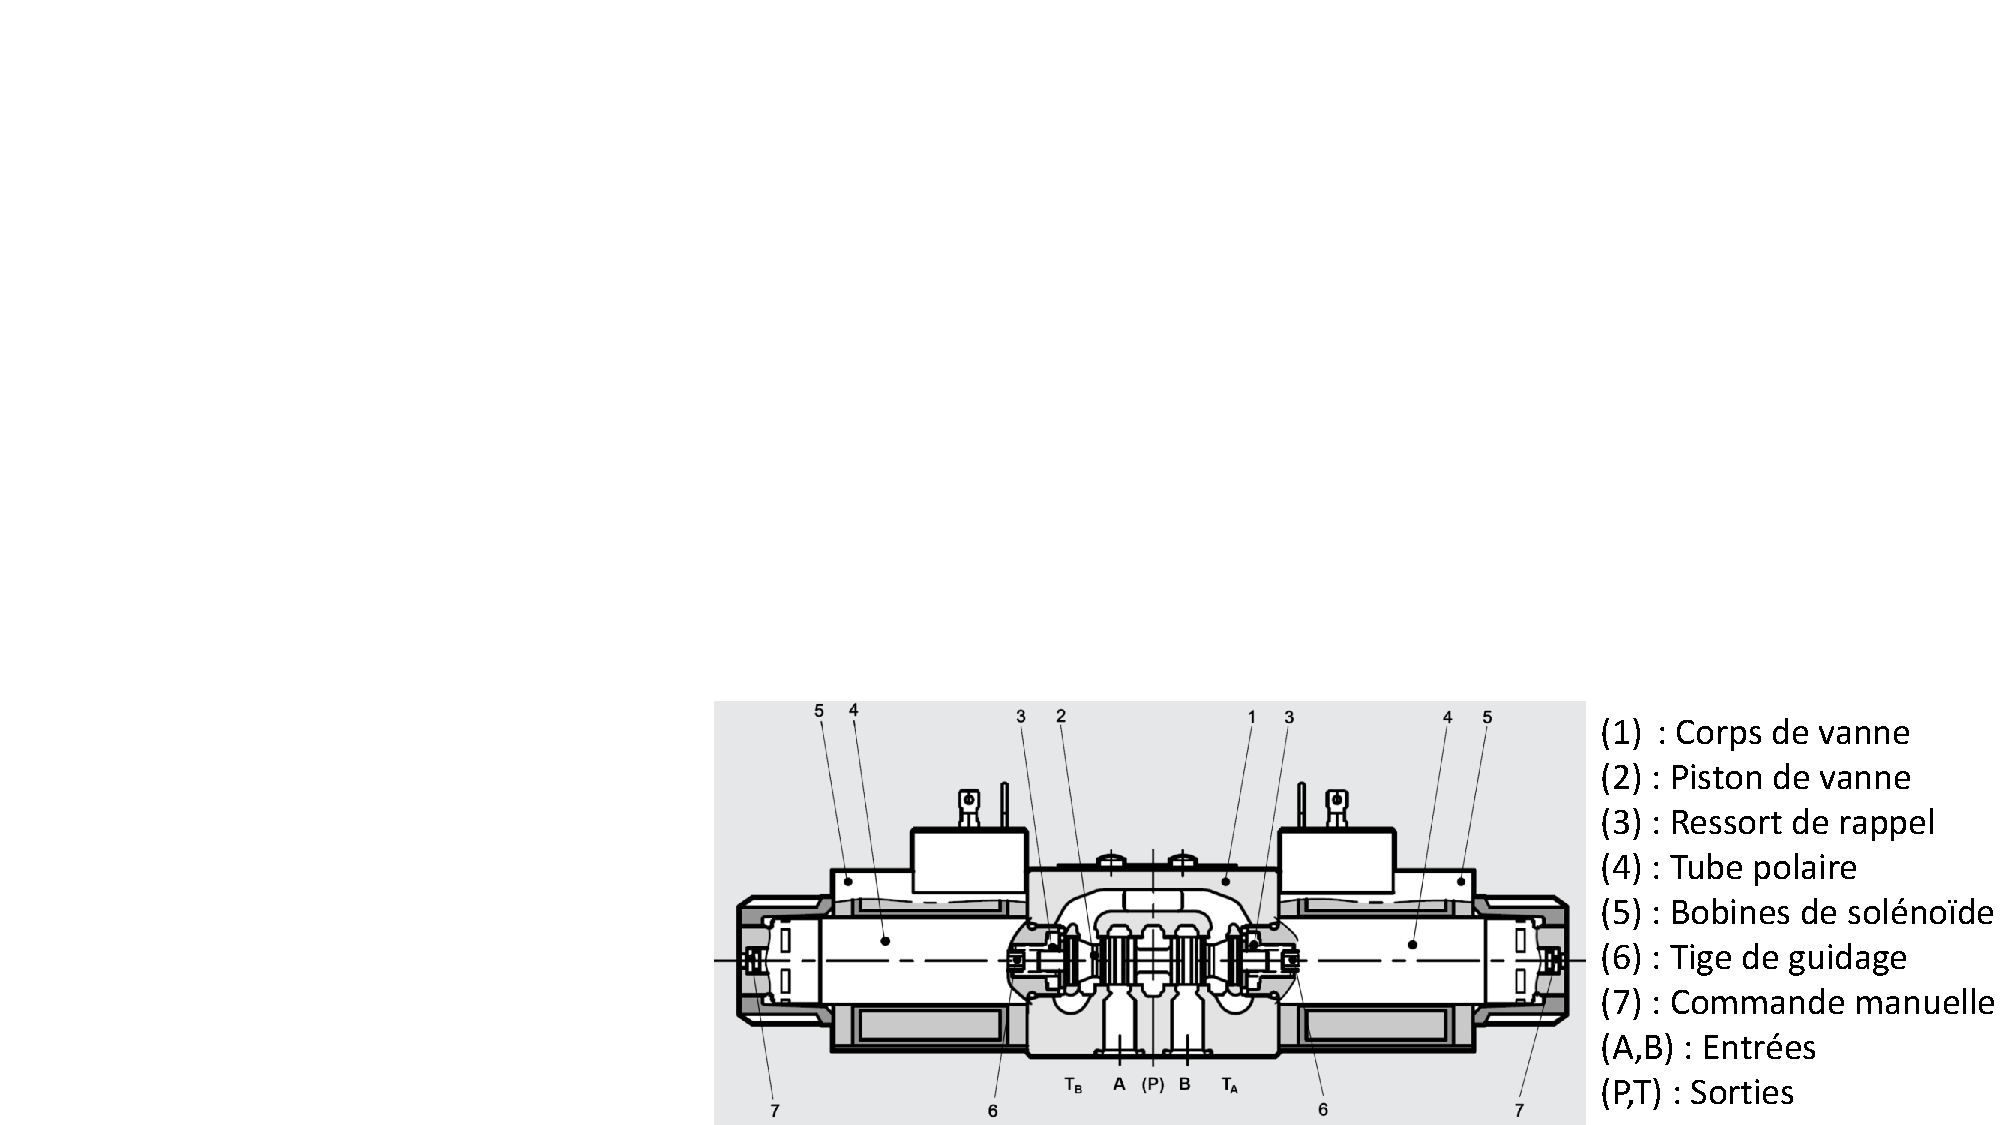
\includegraphics[trim={12.1cm 0cm 0cm 11.9cm},clip,width=0.7\textwidth]{../Chap2/Figure/distributeur_hyd8_Hydrac.pdf}
		\caption{Schéma mécanique d'un distributeur hydraulique 4/2,4/3 à commande électrique/pneumatique \cite{HYDRACINTERNATIONAL2022}}
		\label{fig:distributeur_hyd_HYDRAC}
	\end{center}
\end{figure}		
Il faudra donc soustraire, à l'énergie exploitable, celle nécessaire au pilotage et au fonctionnement de l'aiguillage hydraulique. Ce facteur réduirait l'efficacité de récupération en consommant de l'énergie dans la transformation électrique-mécanique du mouvement du noyau de distribution, dans les frottements durant le déplacement de ce dernier, ainsi que dans son pilotage électrique. L'utilisation d'un distributeur hydraulique à commande électrique risque donc d'induire un effet néfaste non négligeable sur le rendement du récupérateur d'énergie. De plus, sa complexité rendrait difficile sa miniaturisation et par extension, son intégration au système global.

\begin{figure}[!htbp]
	\begin{center}
		\captionsetup{justification=centering}
		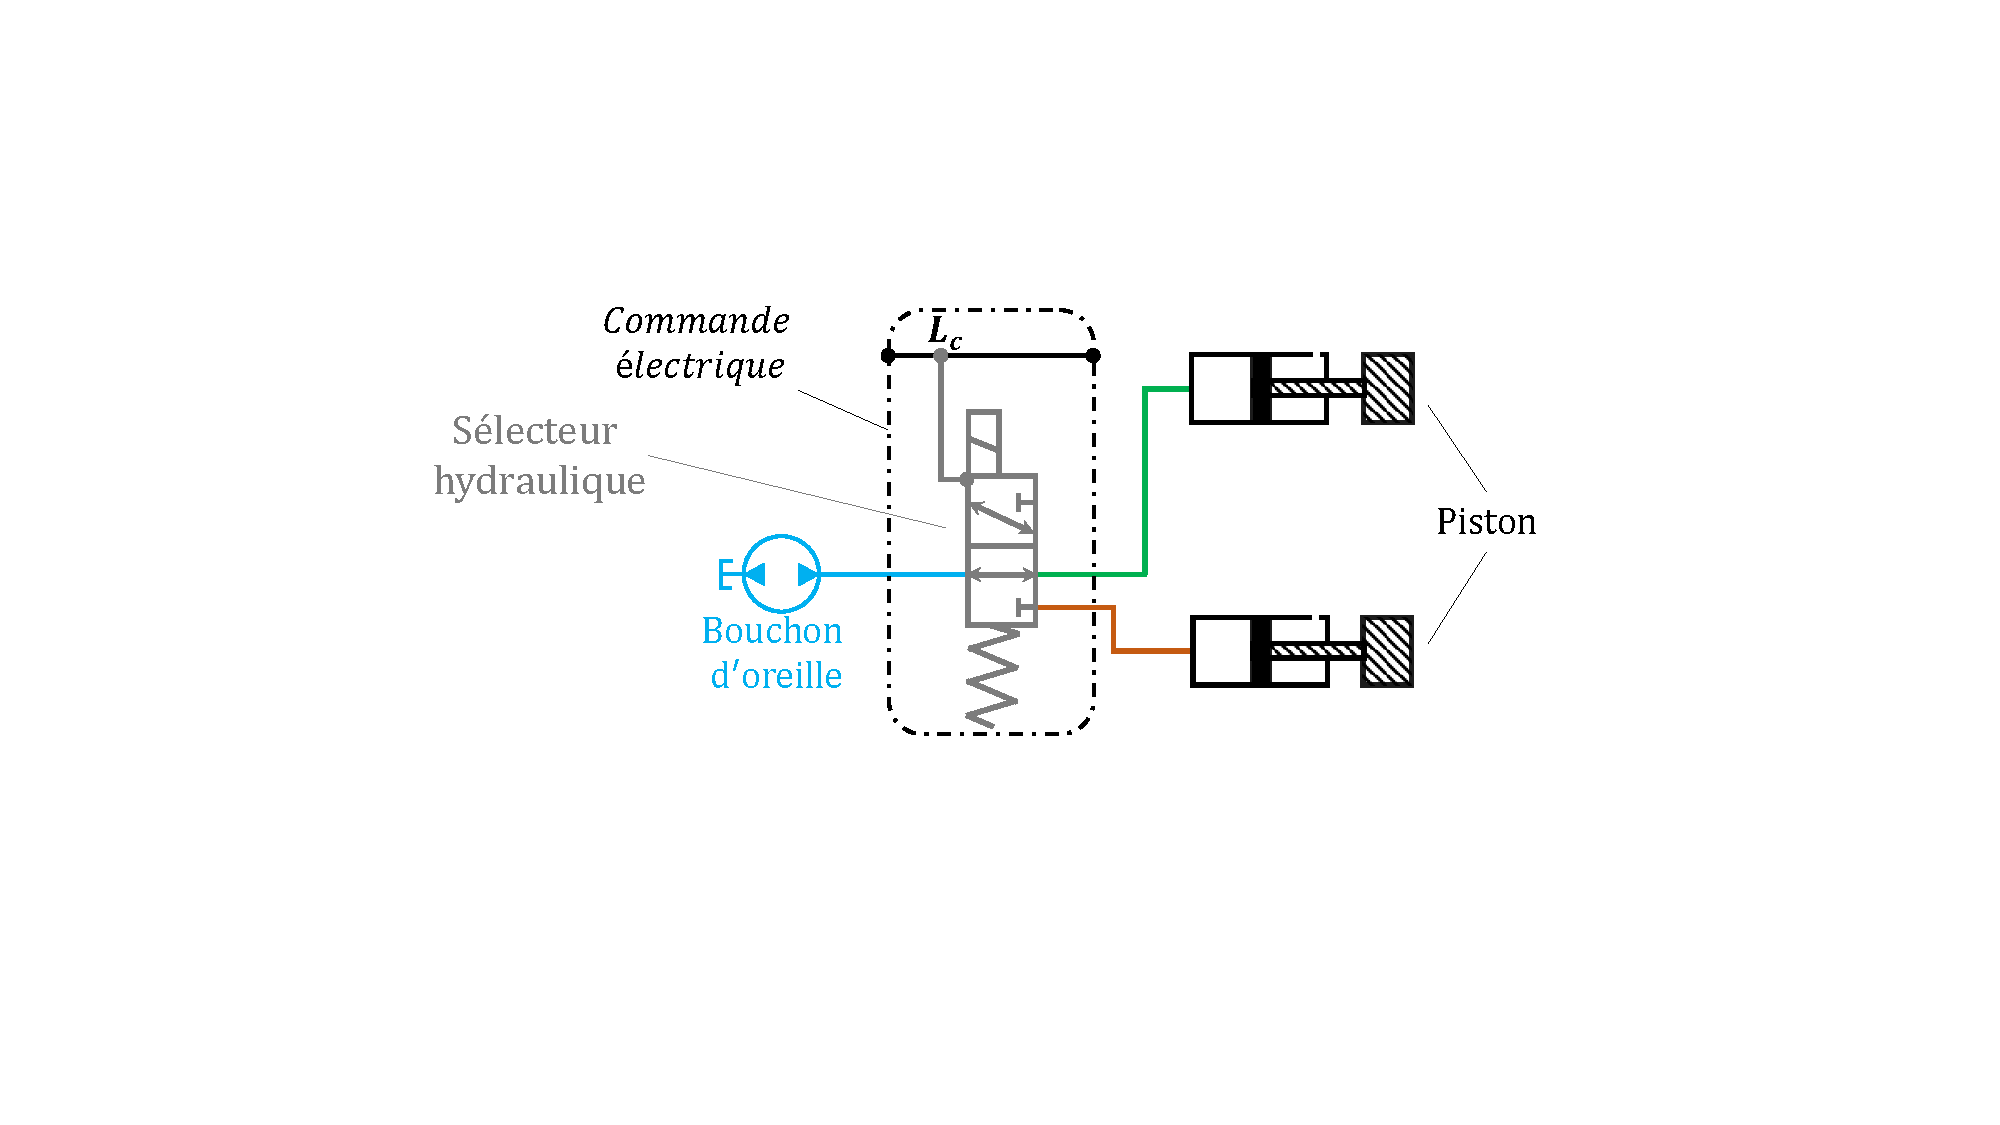
\includegraphics[trim={7cm 6cm 7.5cm 4.9cm},clip,width=0.6\textwidth]{../Chap2/Figure/distributeur_hyd.pdf}
		\caption{Gestion directionnelle d'écoulement par un distributeur hydraulique piloté}
		\label{fig:distributeur_hyd}
	\end{center}
\end{figure}	

Si on considère que plusieurs organes du système de récupération d'énergie sont en mouvement, il devient intéressant d'exploiter directement cette énergie mécanique pour mettre en fonctionnement les VHs. Cela permettrait de s'affranchir de plusieurs étages de transductions, ainsi que d'une commande électronique spécifique. Il semble donc plus pertinent donc de se tourner vers des solutions pouvant être mises en \oe{}uvre directement par ces déplacements mécaniques.

La littérature met en évidence une solution technique à actionnement mécanique qui est schématisée sur la figure \ref{fig:etrangleur_hyd}. Les étrangleurs permettent de générer des PdC dans un écoulement par le moyen d'obstructions mécaniques basées sur la modification de la géométrie du conduit. On dénombre deux grandes familles, les étrangleurs fixes et les étrangleurs variables.

La figure \ref{fig:etrangleur_techno} illustre un exemple d'étrangleur fixe et deux exemples d'étrangleurs variables.
Les PdC générées par un étrangleur fixe sont constantes, car sa géométrie ne peut pas être modifiée. Nous nous tournerons plutôt vers les étrangleurs variables, étant donné que nous aurons besoin successivement d'ouvrir et fermer chacune des valves hydrauliques en fonction de la position de M.
%%%%%%%%%%%%%%%%%%%%%%%%%%
\begin{figure}[!htbp]
	\begin{center}
		\captionsetup{justification=centering}
		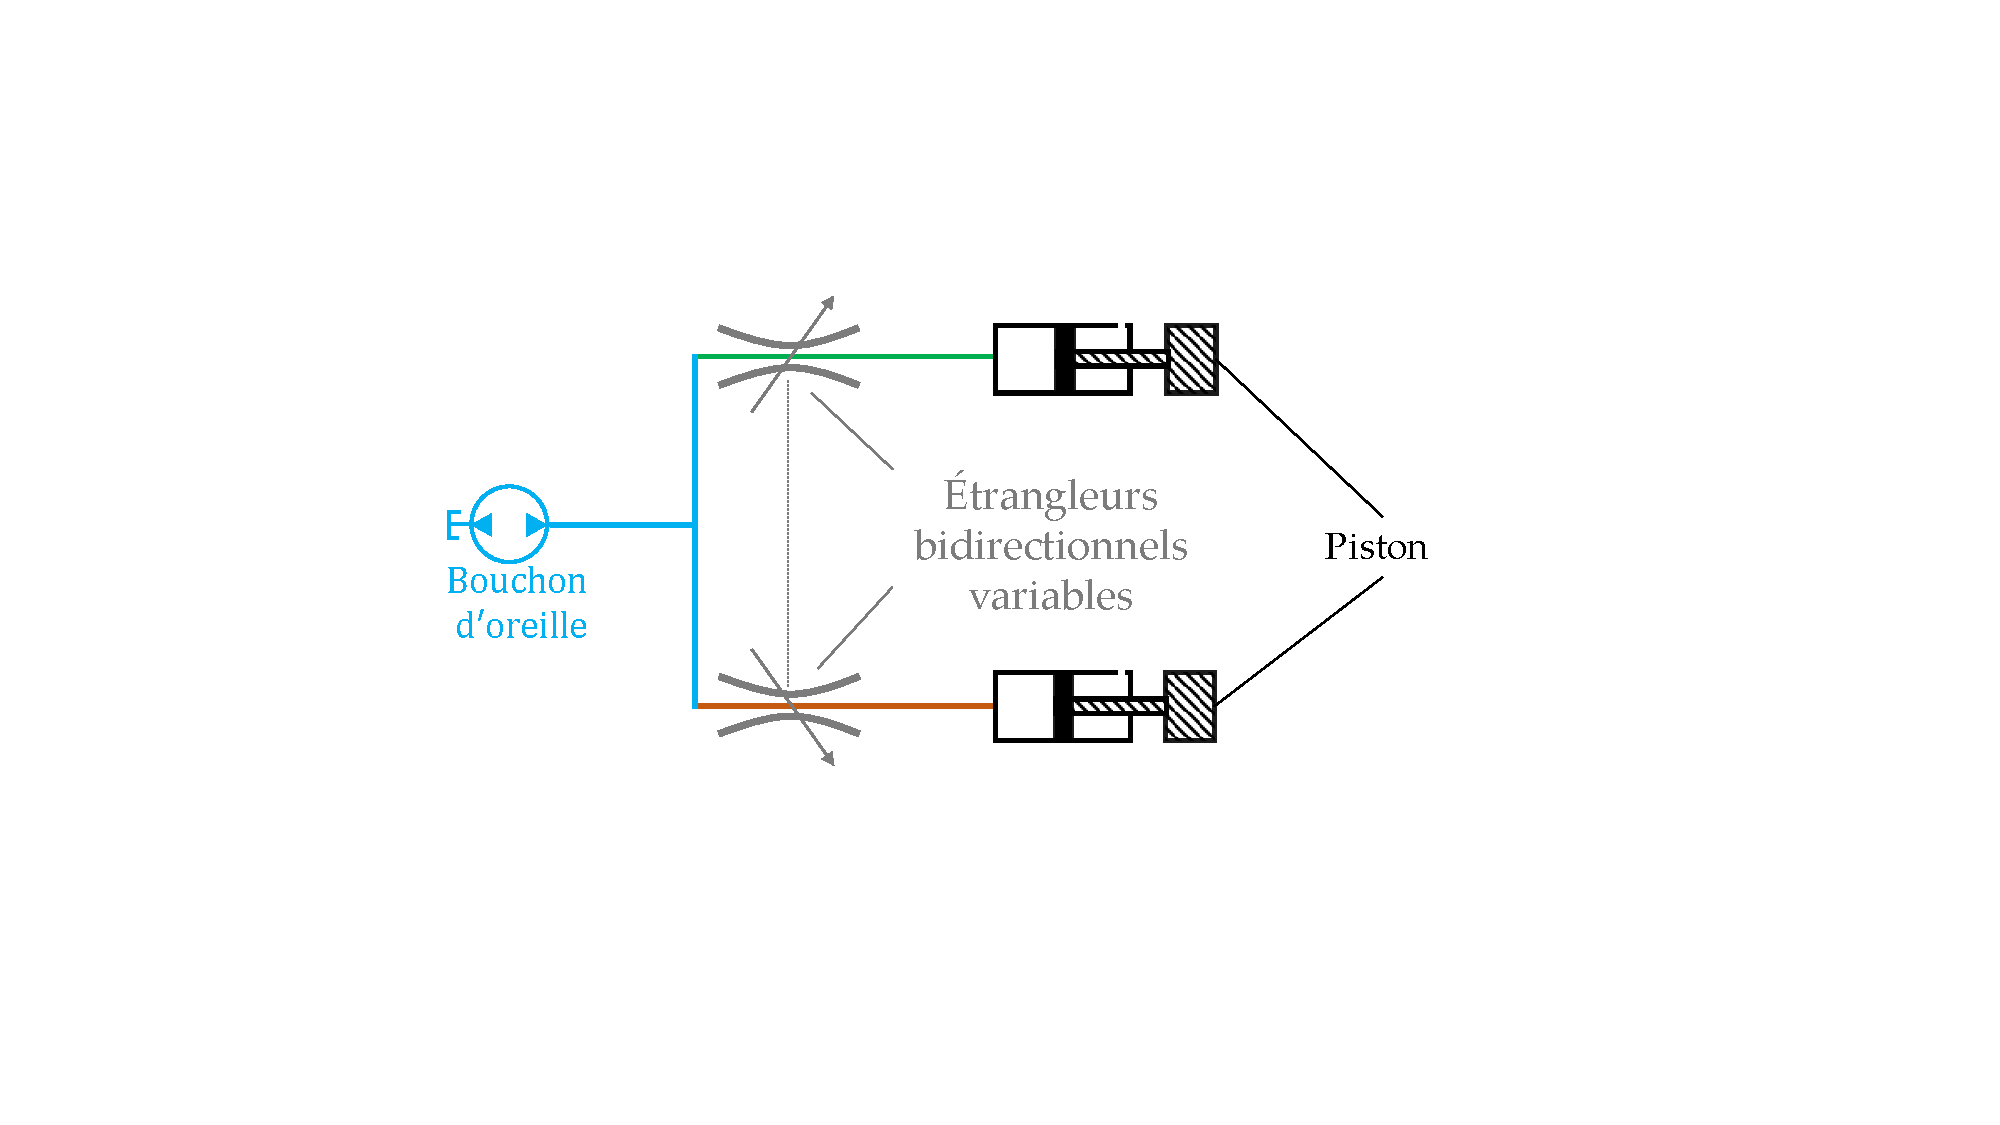
\includegraphics[trim={7cm 6.2cm 9.5cm 5cm},clip,width=0.6\textwidth]{../Chap2/Figure/etrangleur_hyd.pdf}
		\caption{Gestion directionnelle d'écoulement par deux étrangleurs bidirectionnels couplés}
		\label{fig:etrangleur_hyd}
	\end{center}
\end{figure}
%%%%%%%%%%%%%%%%%%%%%%%%%%
%%%%%%%%%%%%%%%%%%%%%%%%%%
\begin{figure}[!htbp]
	\begin{center}
		\begin{subfigure}[t]{0.32\textwidth}
			\captionsetup{justification=centering}
			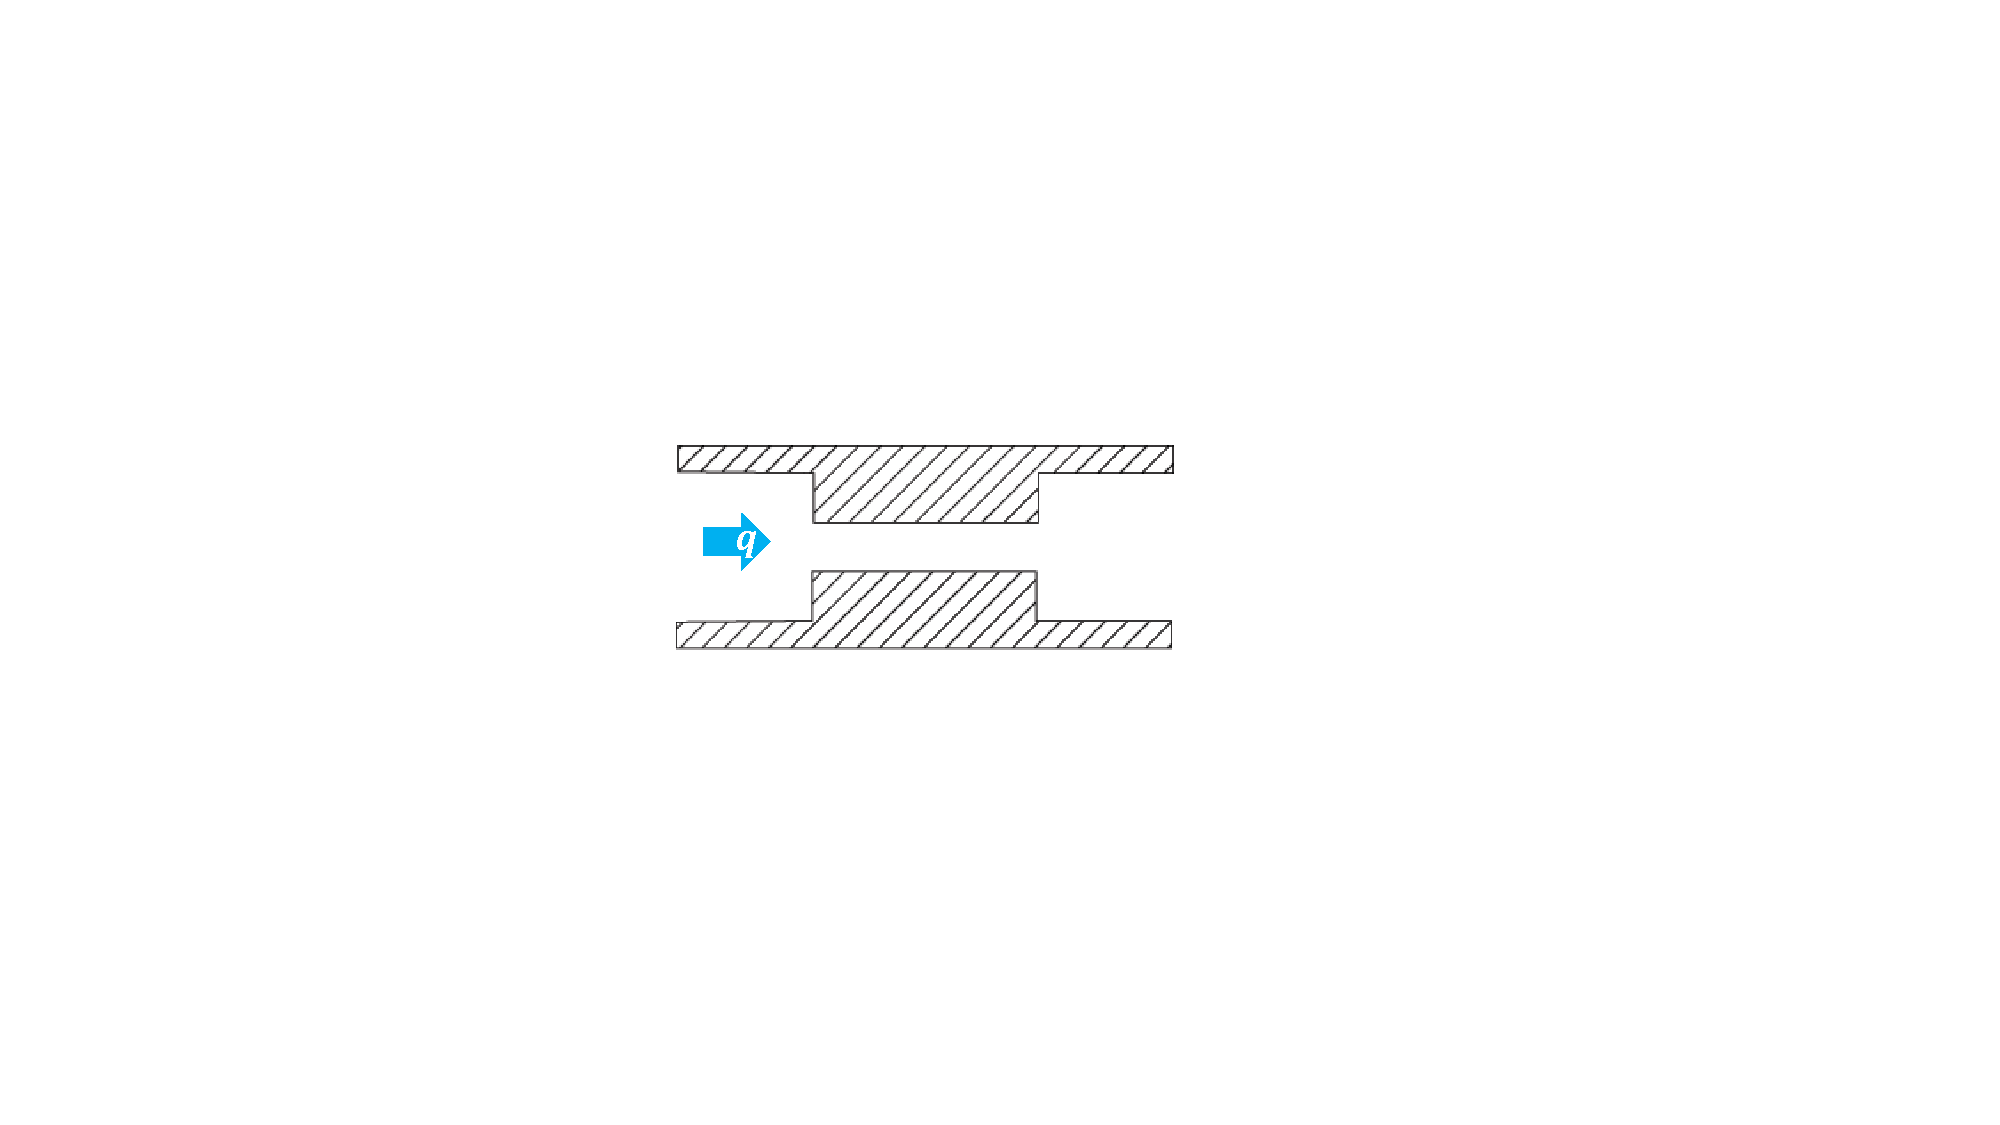
\includegraphics[trim={11cm 6.5cm 13.5cm 7.2cm},clip,width=\textwidth]{../Chap2/Figure/etrangleur_fixe.pdf}
			\caption{Étrangleur fixe à réduction de section brute}
			\label{fig:etrangleur_fixe}
		\end{subfigure}
		\begin{subfigure}[t]{0.3\textwidth}
			\captionsetup{justification=centering}
			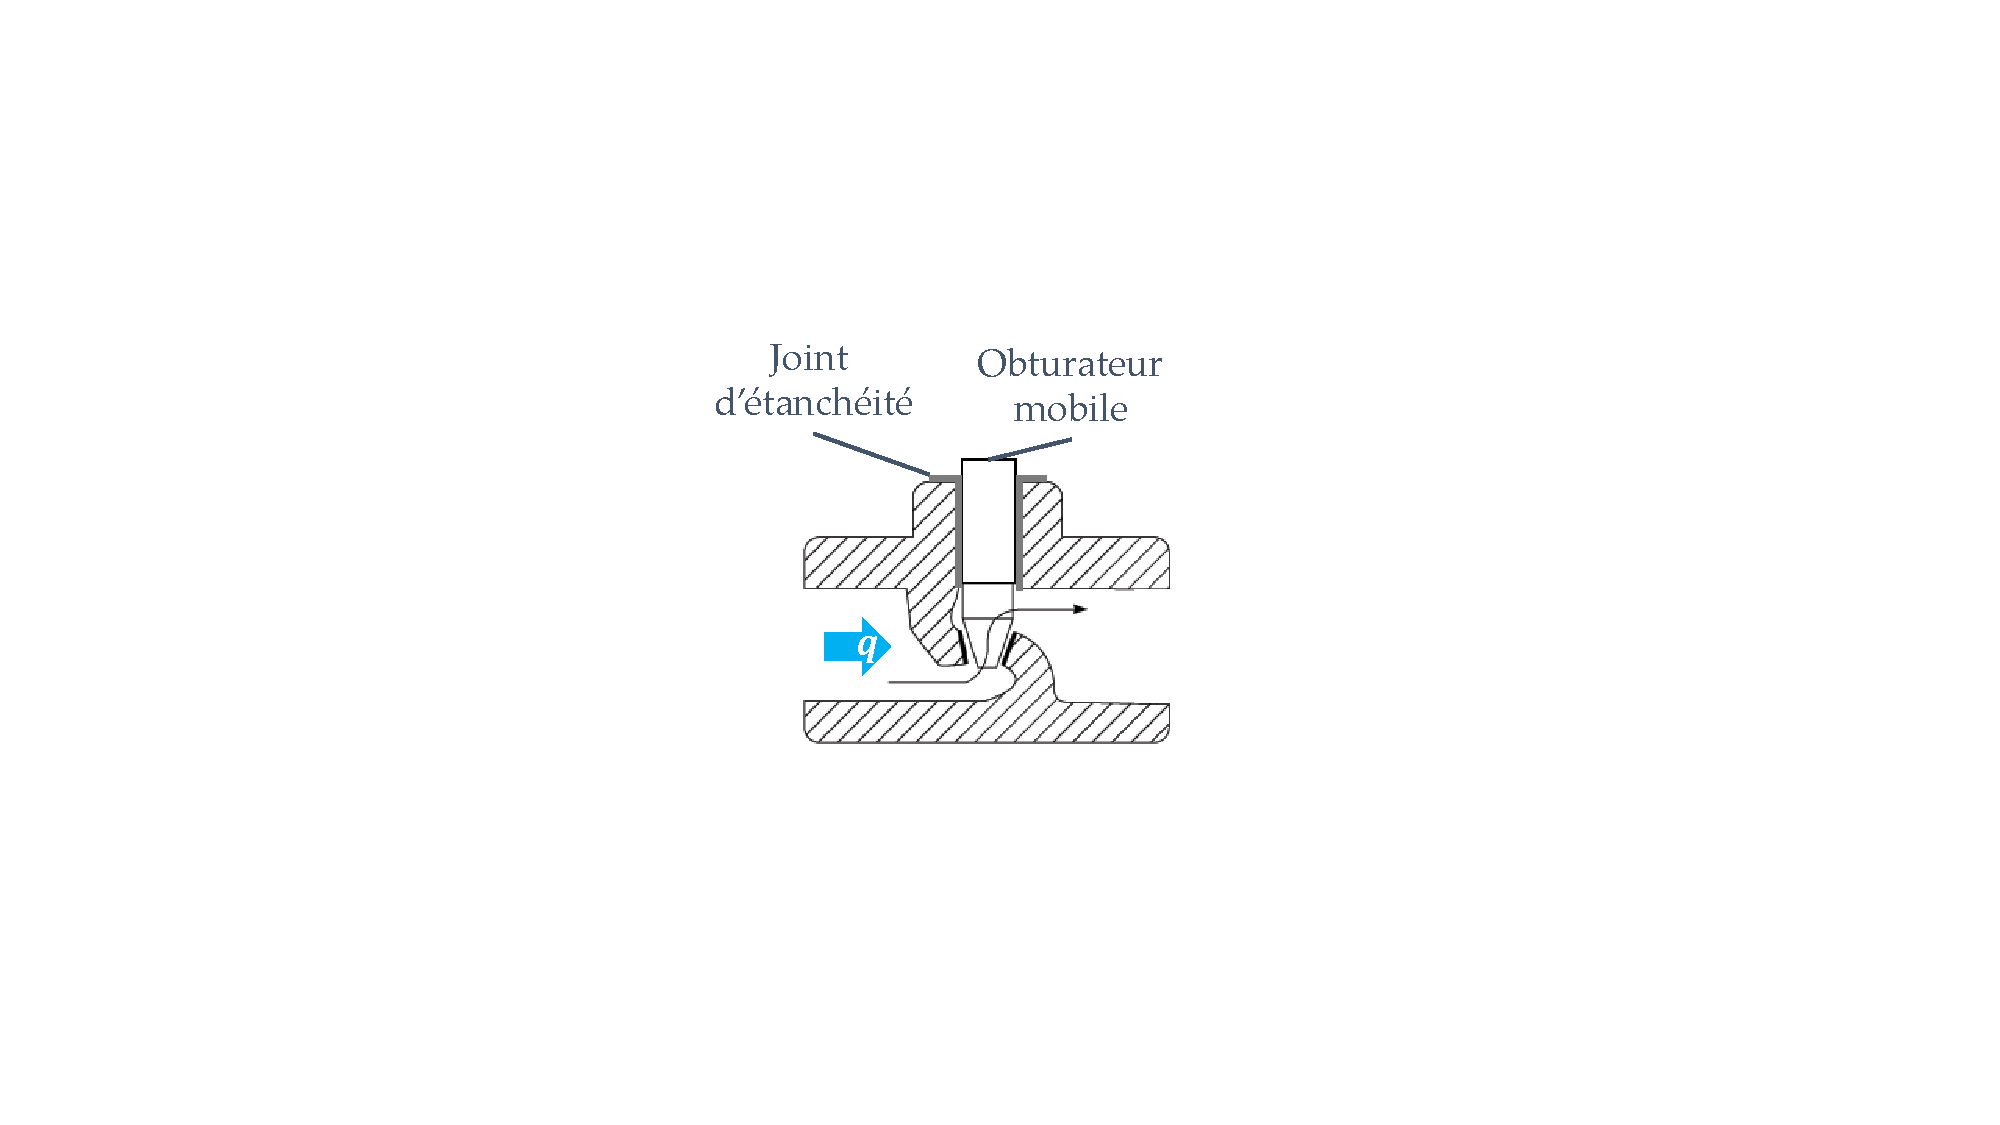
\includegraphics[trim={12cm 6cm 14cm 5.5cm},clip,width=\textwidth]{../Chap2/Figure/etrangleur_pointeau.pdf}
			\caption{Étrangleur variable à pointeau}
			\label{fig:etrangleur_pointeau}
		\end{subfigure}
		\begin{subfigure}[t]{0.34\textwidth}
			\captionsetup{justification=centering}
			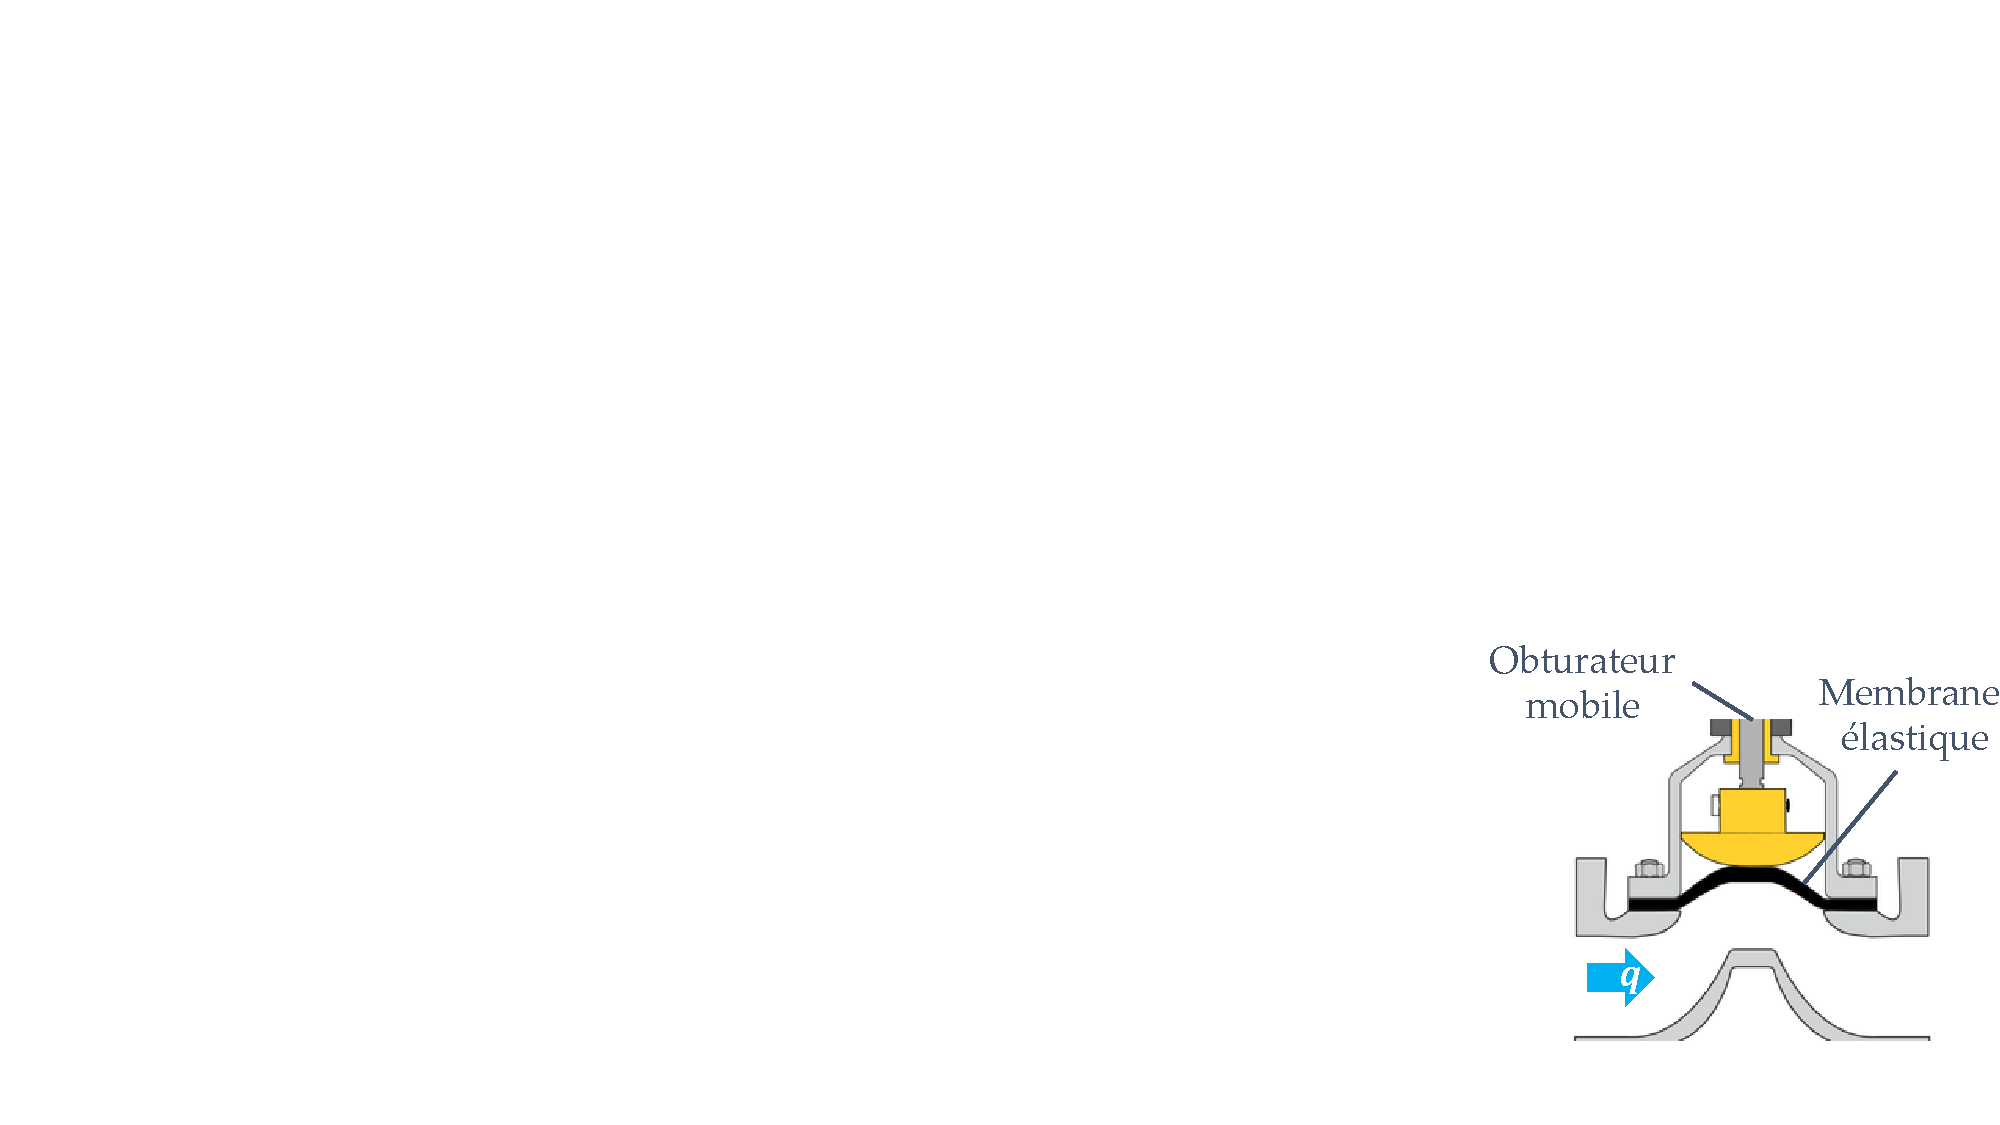
\includegraphics[trim={25cm 1.2cm 0cm 10.6cm},clip,width=\textwidth]{../Chap2/Figure/etrangleur_membrane32.pdf}
			\caption{Étrangleur variable à membrane}
			\label{fig:etrangleur_membrane}
		\end{subfigure}
		\caption{Exemples de solutions technologiques d'étrangleurs hydrauliques \cite{Maxicours2022,Kenovel2022}}
		\label{fig:etrangleur_techno}
	\end{center}
\end{figure}
%%%%%%%%%%%%%%%%

La solution technique de l'étrangleur bidirectionnel variable répondrait au critère hydraulique du cahier des charges pour la conception des VHs. Cependant, les applications courantes (hydraulique industrielle) pour ce choix technique appellent à des solutions technologiques énergivores, car ce critère n'y est pas considéré comme étant important. En effet, les deux exemples illustrés sur les figures \ref{fig:etrangleur_pointeau} et \ref{fig:etrangleur_membrane} fonctionnent à des pressions minimales plus élevées que celles générées dans le bouchon d'oreille, généralement supérieurs à 10kPa. De plus, l'actionnement de l'obturateur mobile nécessite un apport d'énergie externe qui est le plus souvent assuré par une alimentation électrique ou pneumatique. Une partie de cette énergie est dissipée dans le joint d'étanchéité de l'obturateur, ou bien dans l'élasticité de la membrane nécessitant une déformation, en fonction des technologies. Le critère énergétique serait difficile à satisfaire avec ces architectures qui sont caractéristiques des solutions technologiques qui existent dans la famille des étrangleurs variables.

La section qui suit propose alors une nouvelle architecture d'étrangleur variable se basant sur les propriétés de réduction de section locale des tubes flambés en flexion.
	%////////////////////////////////////////////
	\subsection{Solution proposée pour la gestion directionnelle de fluide en mouvement}
	\label{subsec:2.2.3_Solution proposee pour la gestion directionnelle de fluide en mouvement}
	%////////////////////////////////////////////
Les dispositifs d'étranglement à réduction variable sont généralement constituées de plusieurs pièces en mouvement autour d'un joint assurant l'étanchéité du circuit hydraulique. En effet, ces dispositifs sont généralement conçus afin de gérer des volumes de fluide conséquents et donc un certain niveau de fuite est acceptable dans le cadre de leur utilisation conventionnelle. Comme le volume de fluide est fini dans le bouchon d'oreille, l'étanchéité est un critère qui ne peut être négligé pour le circuit hydraulique de notre application. Il nous faudrait alors une structure déformable afin de pouvoir générer une résistance hydraulique en altérant sa géométrie, générant ainsi des PdC similaires à une réduction de section variable. Une telle solution s'affranchit de tout problème d'étanchéité par la continuité physique de la paroi du tube qui contient le fluide. En ce sens, nous nous sommes intéressés aux propriétés statiques et cinématiques de l'étranglement naturellement généré à la section flambée des tubes élastiques. 

Plusieurs études dans la littérature traitent du comportement des écoulements de fluides visqueux au travers de tubes flexibles à parois fines, soumis à des pressions extérieures \cite{Elad1992,Ribeau1994,Heil1996}. Les travaux de Conrad et al. ont contribué à quantifier les pertes de pression engendrées entre l'entrée et la sortie d'une portion de tube flexible flambé. Leurs résultats sont présentés sur la figure \ref{fig:écoulement_tube_écrésé_Conrad1969} \cite{Conrad1969}. Le flambement est causé par une pression trop importante à l’extérieur du tube, comparativement à l'intérieur.
%%%%%%%%%%%%%%%%%%%%%%%%%%%%%%%%%%%
\begin{figure}[!htbp]
	\begin{center}
		\captionsetup{justification=centering}
		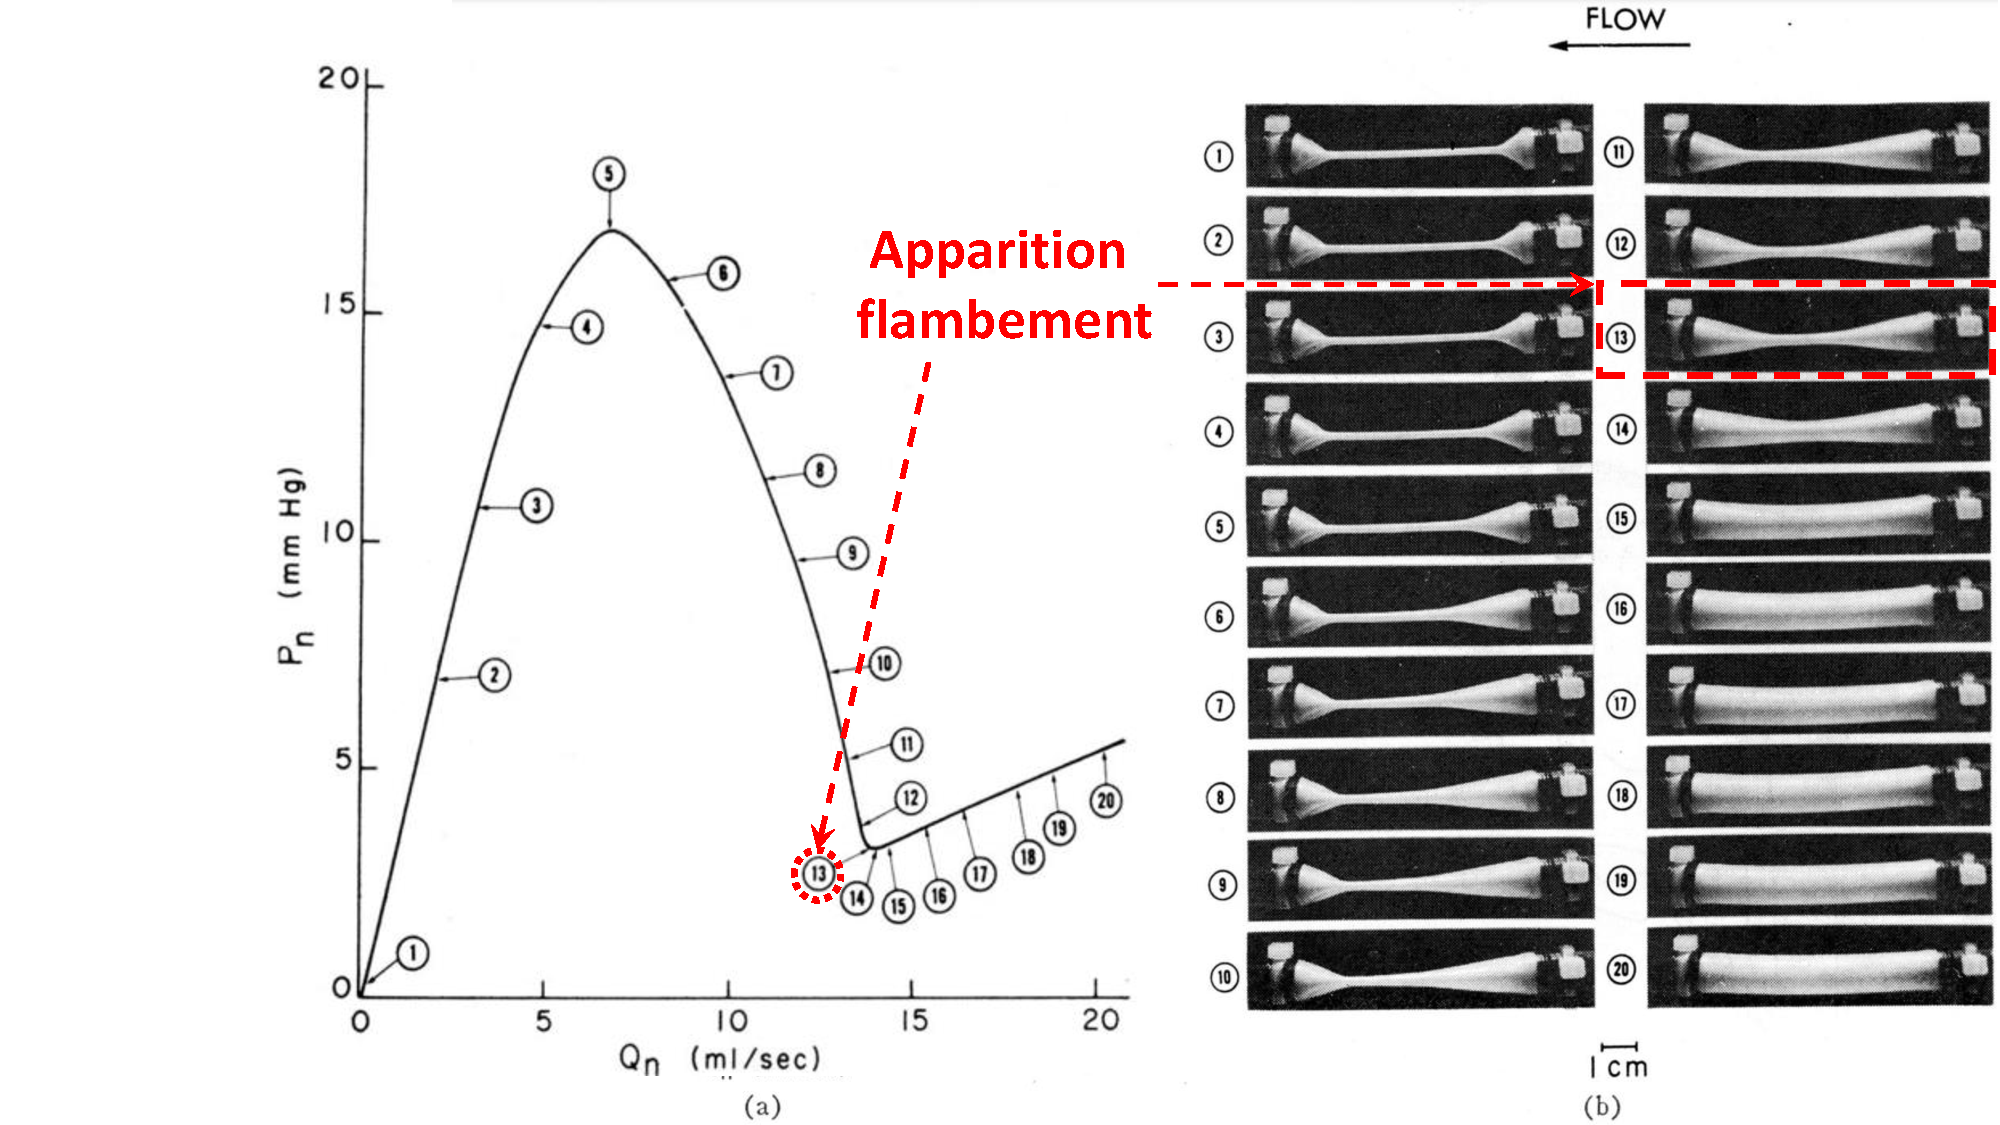
\includegraphics[trim={4cm 0cm 0cm 0cm},clip, 					                 width=\textwidth]{../Chap2/Figure/écoulement_tube_écrésé_Conrad1969.pdf}
		\caption{(a) Pertes de pression ($p_n$) typiques en fonction du débit ($Q_n$) entre l'entrée et la sortie d'un tube en caoutchouc soumis au flambement découlant d'une pression extérieure $p_{ext}$ constante engendrant une contraction locale. (b) Vue de côté du tube en flambement aux positions statiques indiquées sur la figure de gauche. \cite{Conrad1969}}
		\label{fig:écoulement_tube_écrésé_Conrad1969}
	\end{center}
\end{figure}
%%%%%%%%%%%%%%%%%%%%%%%%%%%%%%%%%%%
Le protocole d'essai consistait à augmenter la pression $p_1$ en entrée du tube sur 20 niveaux. La figure \ref{fig:écoulement_tube_écrésé_Conrad1969}.a a alors pu être établie en mesurant la pression $p_2$ en aval et en mesurant le débit $Q_n$ traversant le tube pour chaque incrément de $p_1$. Si on considère les incréments dans le sens décroissant, le phénomène de flambement semble apparaître pour le point d'incrément n°13. L'information pertinente se situe après le flambement, soit entre le 13e et 5e incrément. La perte de pression engendrée par le tube flambé augmente alors d'autant plus que le niveau de flambement augmente. Les incréments 1-5 correspondent au cas où $p_1<p_{ext}$, le tube est alors considéré obstrué. 
%En effet, les pertes de pression induites sont théoriquement directement proportionnelles au débit de l'écoulement, elles deviennent alors faibles lorsque le débit diminue sous un certain seuil. Dans cette étude ce seuil semble être d'environ $7.5$ml/sec. La relation théorique entre les pertes de pression et le débit sera explicité plus tard dans la modélisation hydraulique du circuit implémenté dans notre système. 
Cette étude montre donc qu'un tube flexible flambé peut agir comme une valve fermée pour un certain niveau de flambement qui dépend de sa géométrie initiale. En effet, un écoulement peut être fortement réduit, voire stoppé, lorsqu'il rencontre une section flambée, comme celles illustrées sur la figure \ref{fig:tuyau_arrosage} pour des cas extrêmes.
%%%%%%%%%%%%%%%%%%%%%%%%%%%%%%%%%%%
\begin{figure}[!htbp]
\begin{center}
    \captionsetup{justification=centering}
	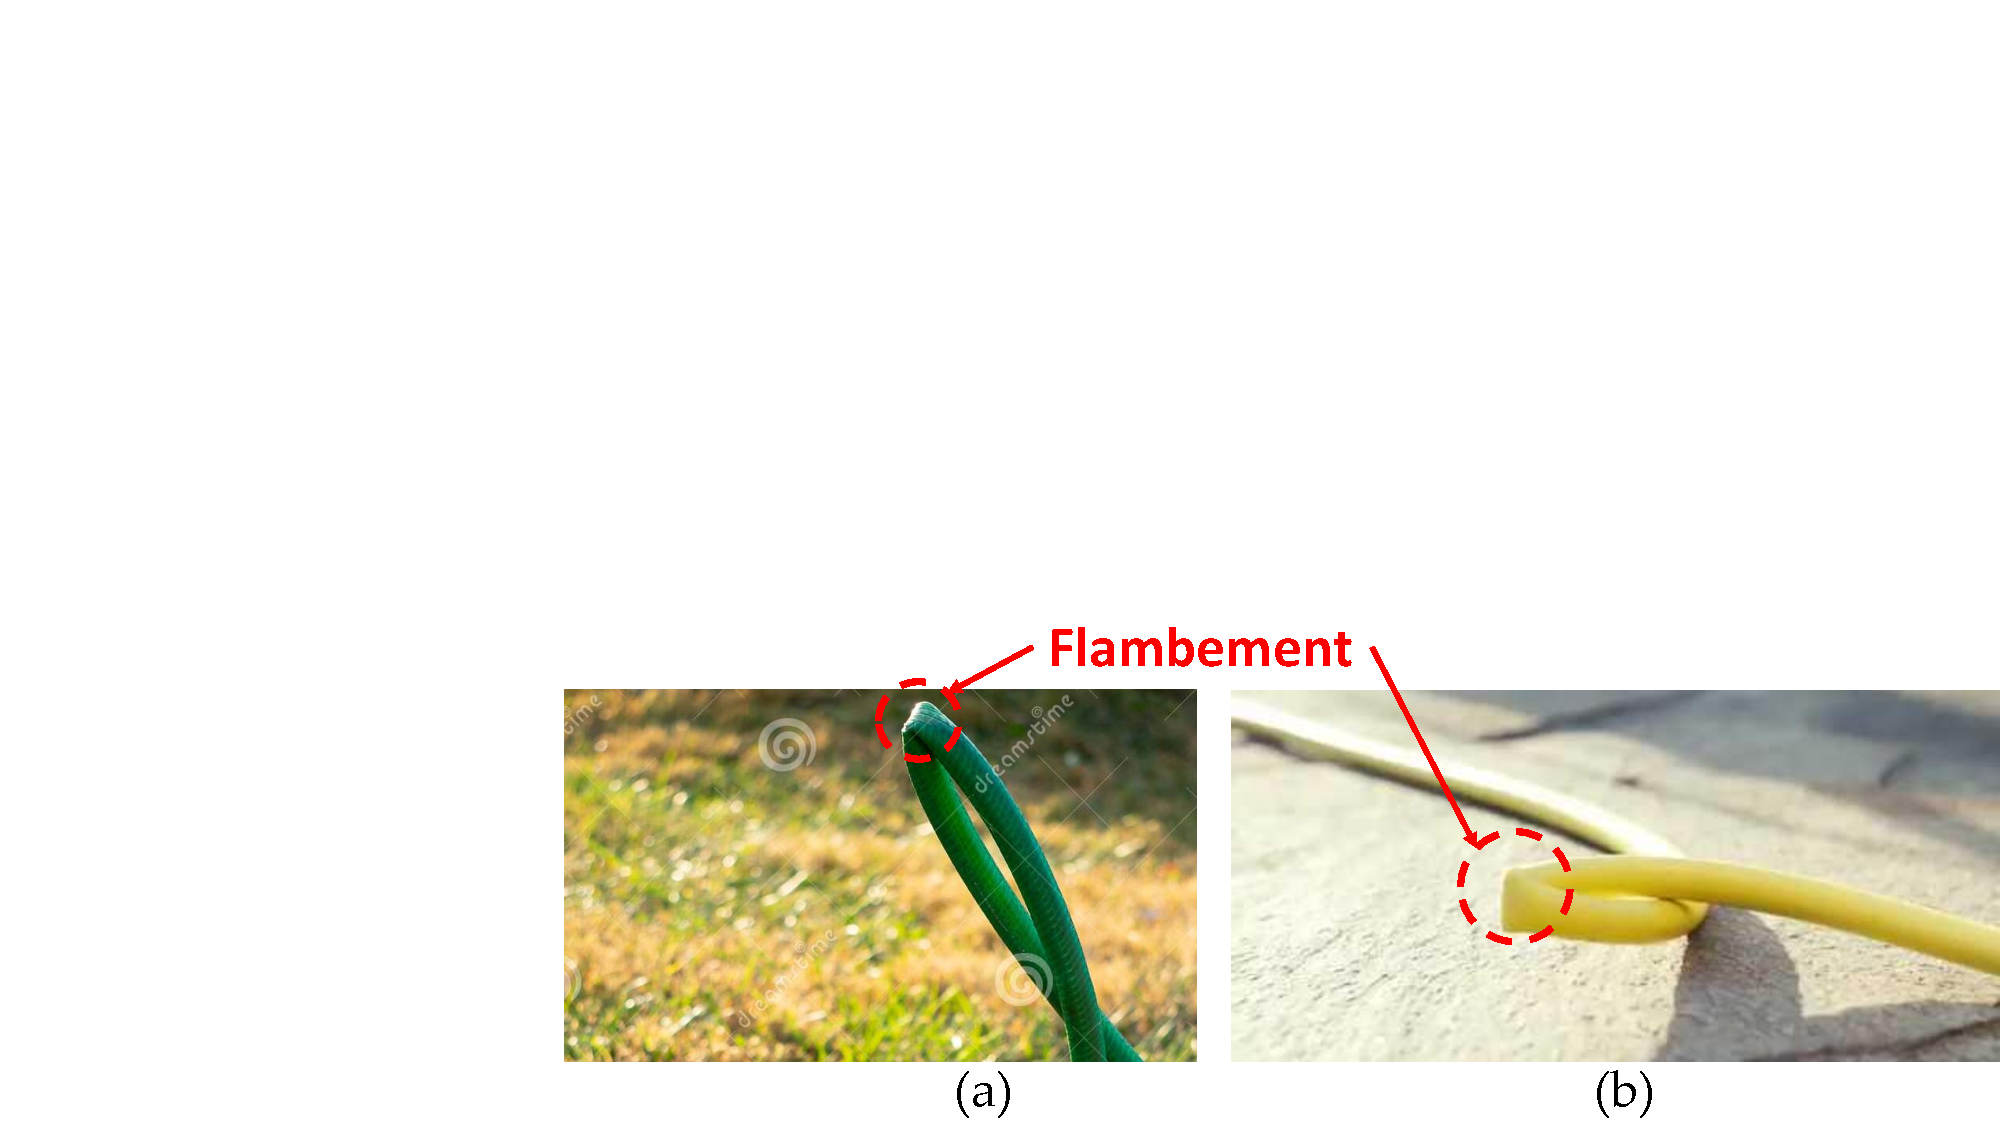
\includegraphics[trim={9cm 0cm 0cm 10cm},clip, 					                 width=0.6\textwidth]{../Chap2/Figure/tuyau_arrosage.pdf}
	\caption{Exemples de tubes flexibles flambés \cite{SMARTFLEXGarden2019,Blessingscaptured2022}.}
	\label{fig:tuyau_arrosage}
\end{center}	
\end{figure}
%%%%%%%%%%%%%%%%%%%%%%%%%%%%%%%%%%%
Ce flambement peut être engendré sur un tube flexible par une pression extérieure relative supérieure à la pression interne du tube, par une action mécanique directe en pinçant le tube, ou bien, en lui imposant une flexion comme c'est le cas sur la figure \ref{fig:tuyau_arrosage}. L'intégrabilité d'une telle solution technologique comme organe remplissant le rôle de VH pour notre application peut alors être envisagée. Le tube flambé présente en effet deux principaux avantages comparé aux solutions classiques introduites précédemment. La première est la facilité de fabrication et de fonctionnement basée sur la seule flexion d'un simple tube. La seconde est l'étanchéité assurée par l'absence de pièces en mouvement au sein du fluide en écoulement, mais aussi par la continuité physique de la paroi du tube qui contient le fluide.

Compte tenu des besoins du système, nous proposons une nouvelle architecture d'étrangleur hydraulique, constituée d'une portion de tube flexible soumis à la flexion au delà du point de flambement par action mécanique externe. Le pliage de la VH pourra être assuré par le mouvement de la masse M. La figure \ref{fig:detail_flambement_MDOB} schématise la configuration de pliage d'une telle valve implémentée sur l'OB. La VH se compose ainsi de deux gaines rigides au travers desquelles est fixée la portion de tube flexible. Une des gaines est fixe et l'autre pivote autour du point de flambement de la VH, grâce à l'action mécanique générée par le mouvement de M le long de son axe d'oscillation (axe $\vec{x}$).
%%%%%%%%%%%%%%%%%%%%%%%%%%%%%%%%%%%
\begin{figure}[!htb]
	\begin{center}
		\captionsetup{justification=centering}
		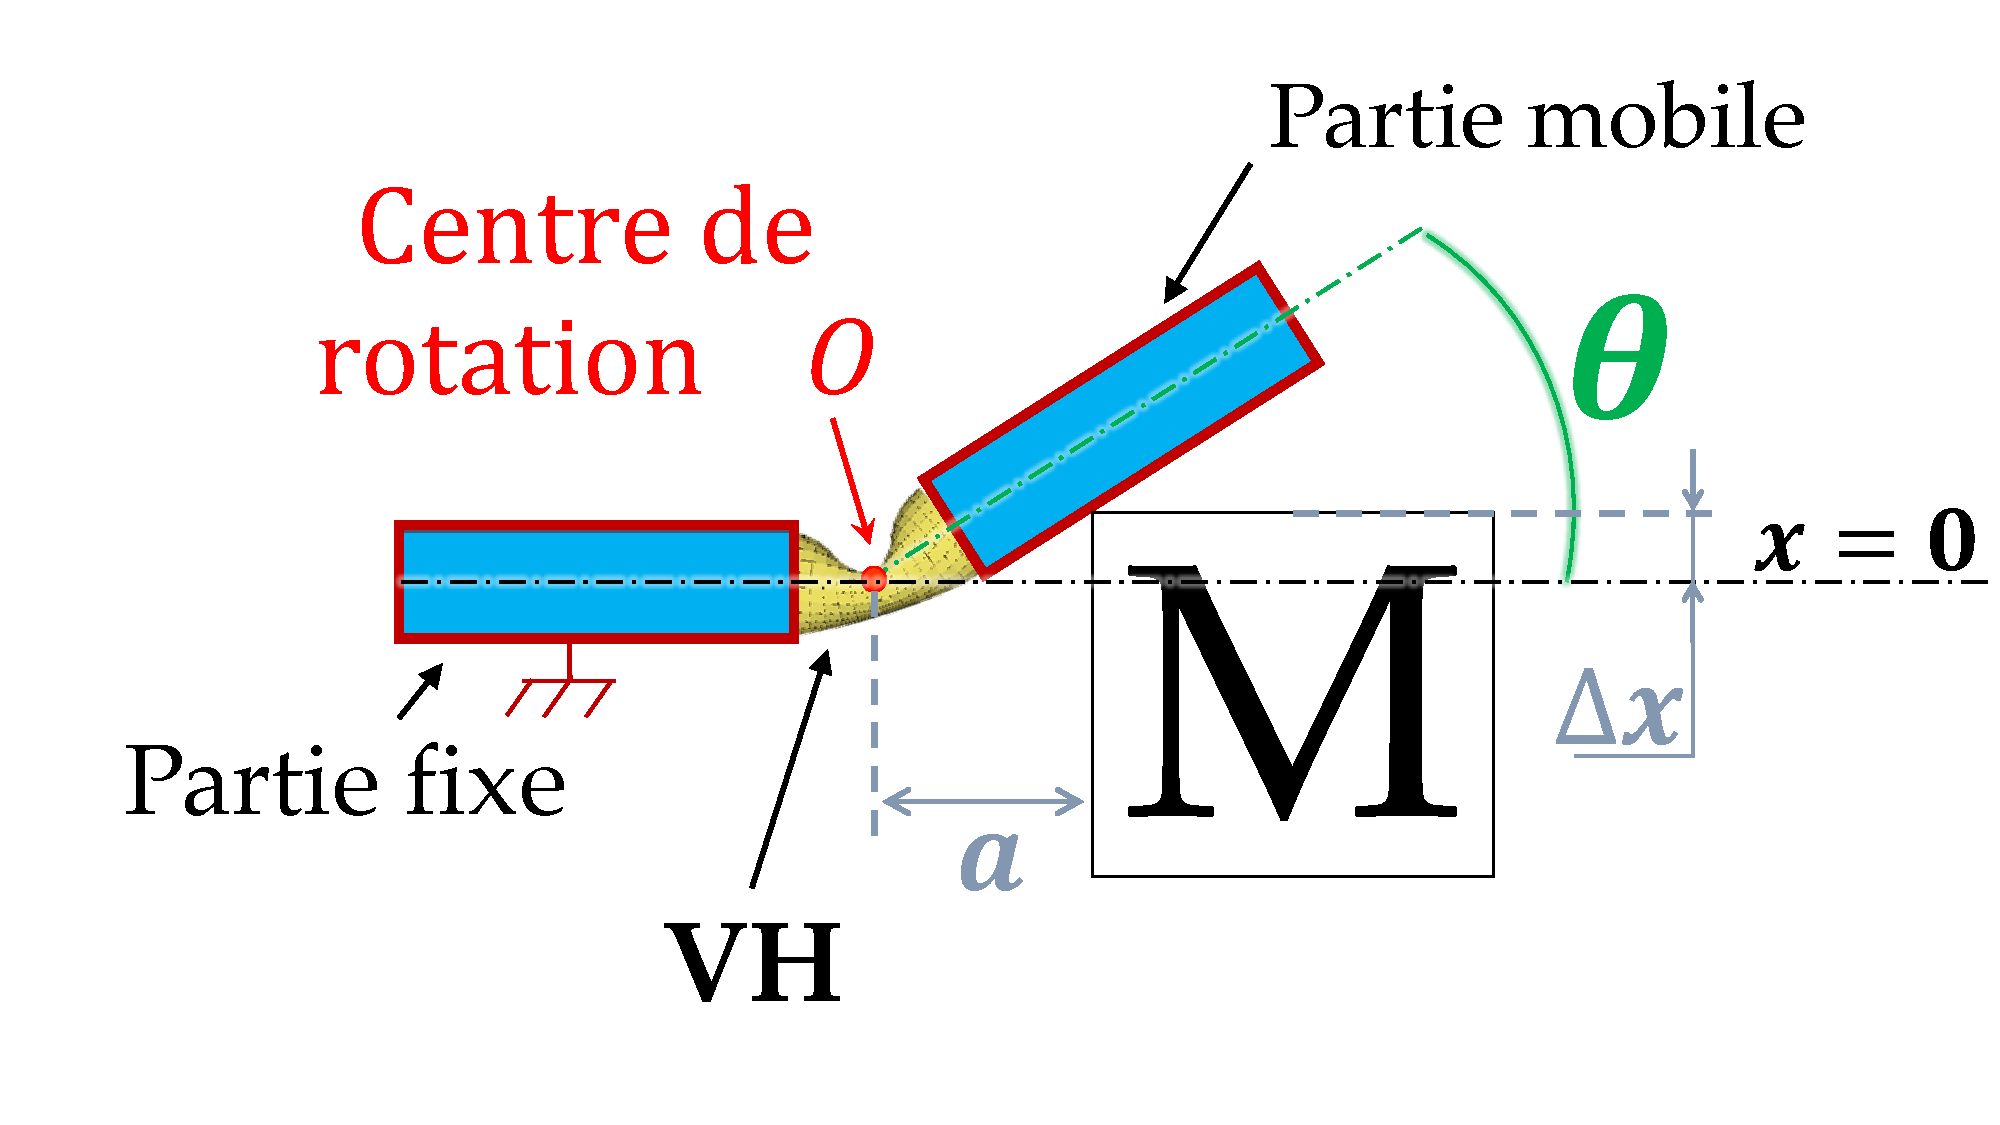
\includegraphics[trim={2cm 2cm 3cm 1cm},clip,width=0.5\textwidth]{../Chap2/Figure/detail_flambement_MDB.pdf}
		\caption{Détail du fonctionnement de la VH en tube flexible}
		\label{fig:detail_flambement_MDOB}
	\end{center}
\end{figure}
%%%%%%%%%%%%%%%%%%%%%%%%%%%%%%%%%%%

On peut aisément calculer l'angle de flexion $\theta$ de la VH en fonction du déplacement $\Delta x$ de M si on fixe le bras de levier de pliage $a$, en supposant que le point de rotation $O$ est centré en $x=0$. L'angle $\theta$ s'exprime alors par l'équation \ref{eq:theta=f(x_m)}.
\begin{equation}
	\theta = \arctan \biggl( \frac{\Delta x}{a} \biggr)
	\label{eq:theta=f(x_m)}
\end{equation}
L'action de pliage de la VH induira une raideur additionnelle à celle de l'OB suivant l'axe d'oscillation $\vec{x}$. Celle-ci sera quantifiée et dimensionnée par la suite afin de ne pas perturber le caractère bistable de l'oscillateur. Cette énergie étant élastique, elle n'induira théoriquement pas de pertes énergétiques. Cependant, le frottement entre M et la gaine rigide mobile sera dissipatif par frottements. De plus, il y aura de la dissipation d'énergie intrinsèque au matériau composant la portion de tube flexible en déformation.

Il faudra intégrer les deux valves hydrauliques de façon symétrique. Le mouvement de M étant symétrique par rapport à sa position d'équilibre instable en $x=0$, on se propose d'intégrer les VHs suivant la configuration schématisée sur la figure \ref{fig:integration_VH_face} en vue de face. Le schéma cinématique montrant uniquement l'OB et les VHs en vue de dessus est également présenté sur la figure \ref{fig:integration_VH_dessus}. La dynamique d'ouverture et de fermeture couplée des valves avec cette configuration permet théoriquement le cyclage du mouvement de M suivant les phases de fonctionnement qui ont été décrites précédemment. Cette architecture \emph{frequency-up} de récupérateur d'énergie hydraulique, auto-cyclé par des VH en tubes flambés, pour les applications intra-auriculaires, a fait l'objet d'un dépôt de brevet aux États-Unis au cours de la thèse \cite{Avetissian2021}. Ce dernier a été déposé dans le cadre de la collaboration entre l'Université Savoie Mont Blanc et l'École de Technologie Supérieure de Montréal.
%%%%%%%%%%%%%%%%%%%%%%%%%%%%%%%%%%
\begin{figure}[!htb]
	\begin{center}
		\captionsetup{justification=centering}
		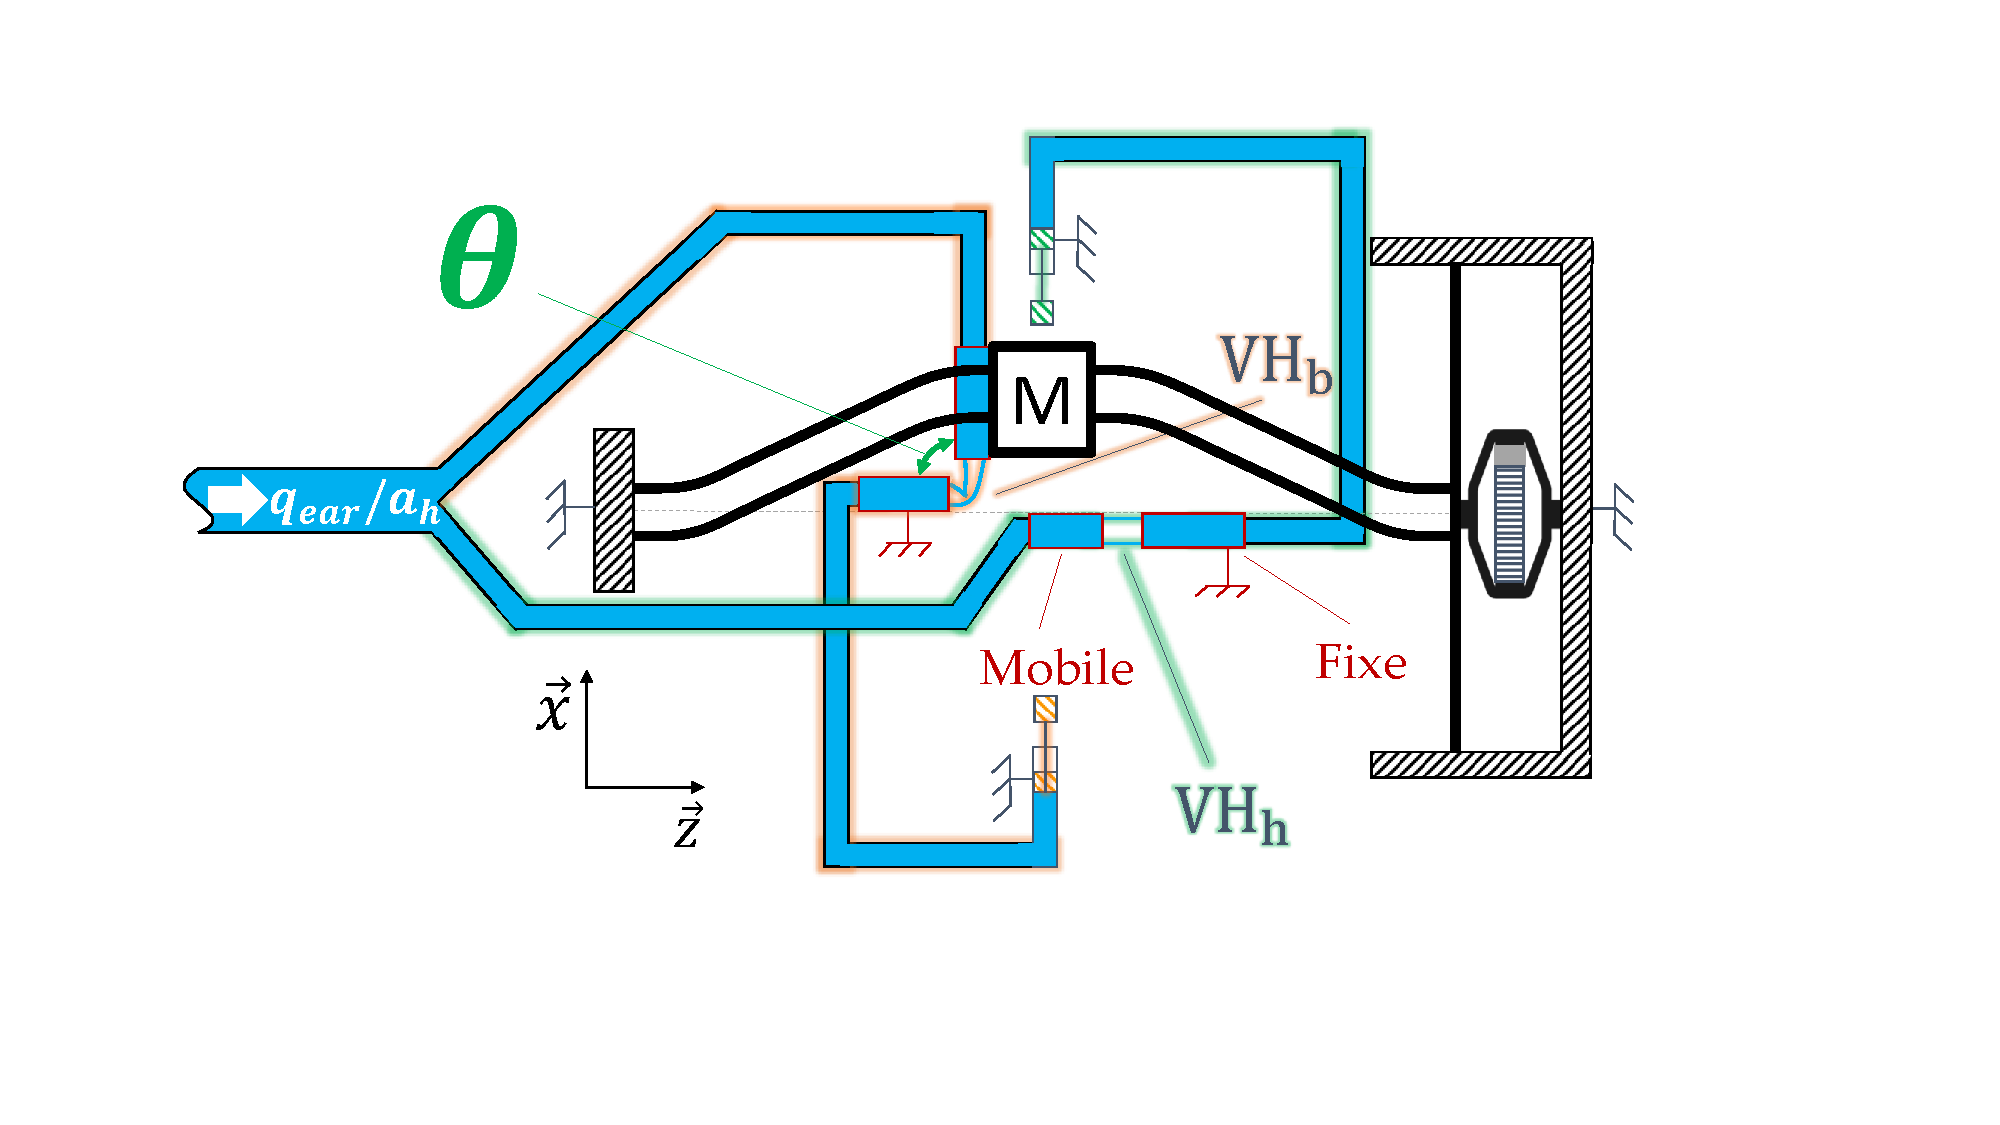
\includegraphics[trim={3cm 4cm 6cm 2cm},clip,width=0.8\textwidth]{../Chap2/Figure/integration_VH_face.pdf}
		\caption{Intégration VHs - Vue de face}
		\label{fig:integration_VH_face}
	\end{center}
\end{figure}
%%%%%%%%%%%%%%%%%%%%%%%%%%%%%%%%%%
%%%%%%%%%%%%%%%%%%%%%%%%%%%%%
\begin{figure}[!htbp]
	\begin{center}
		\captionsetup{justification=centering}
		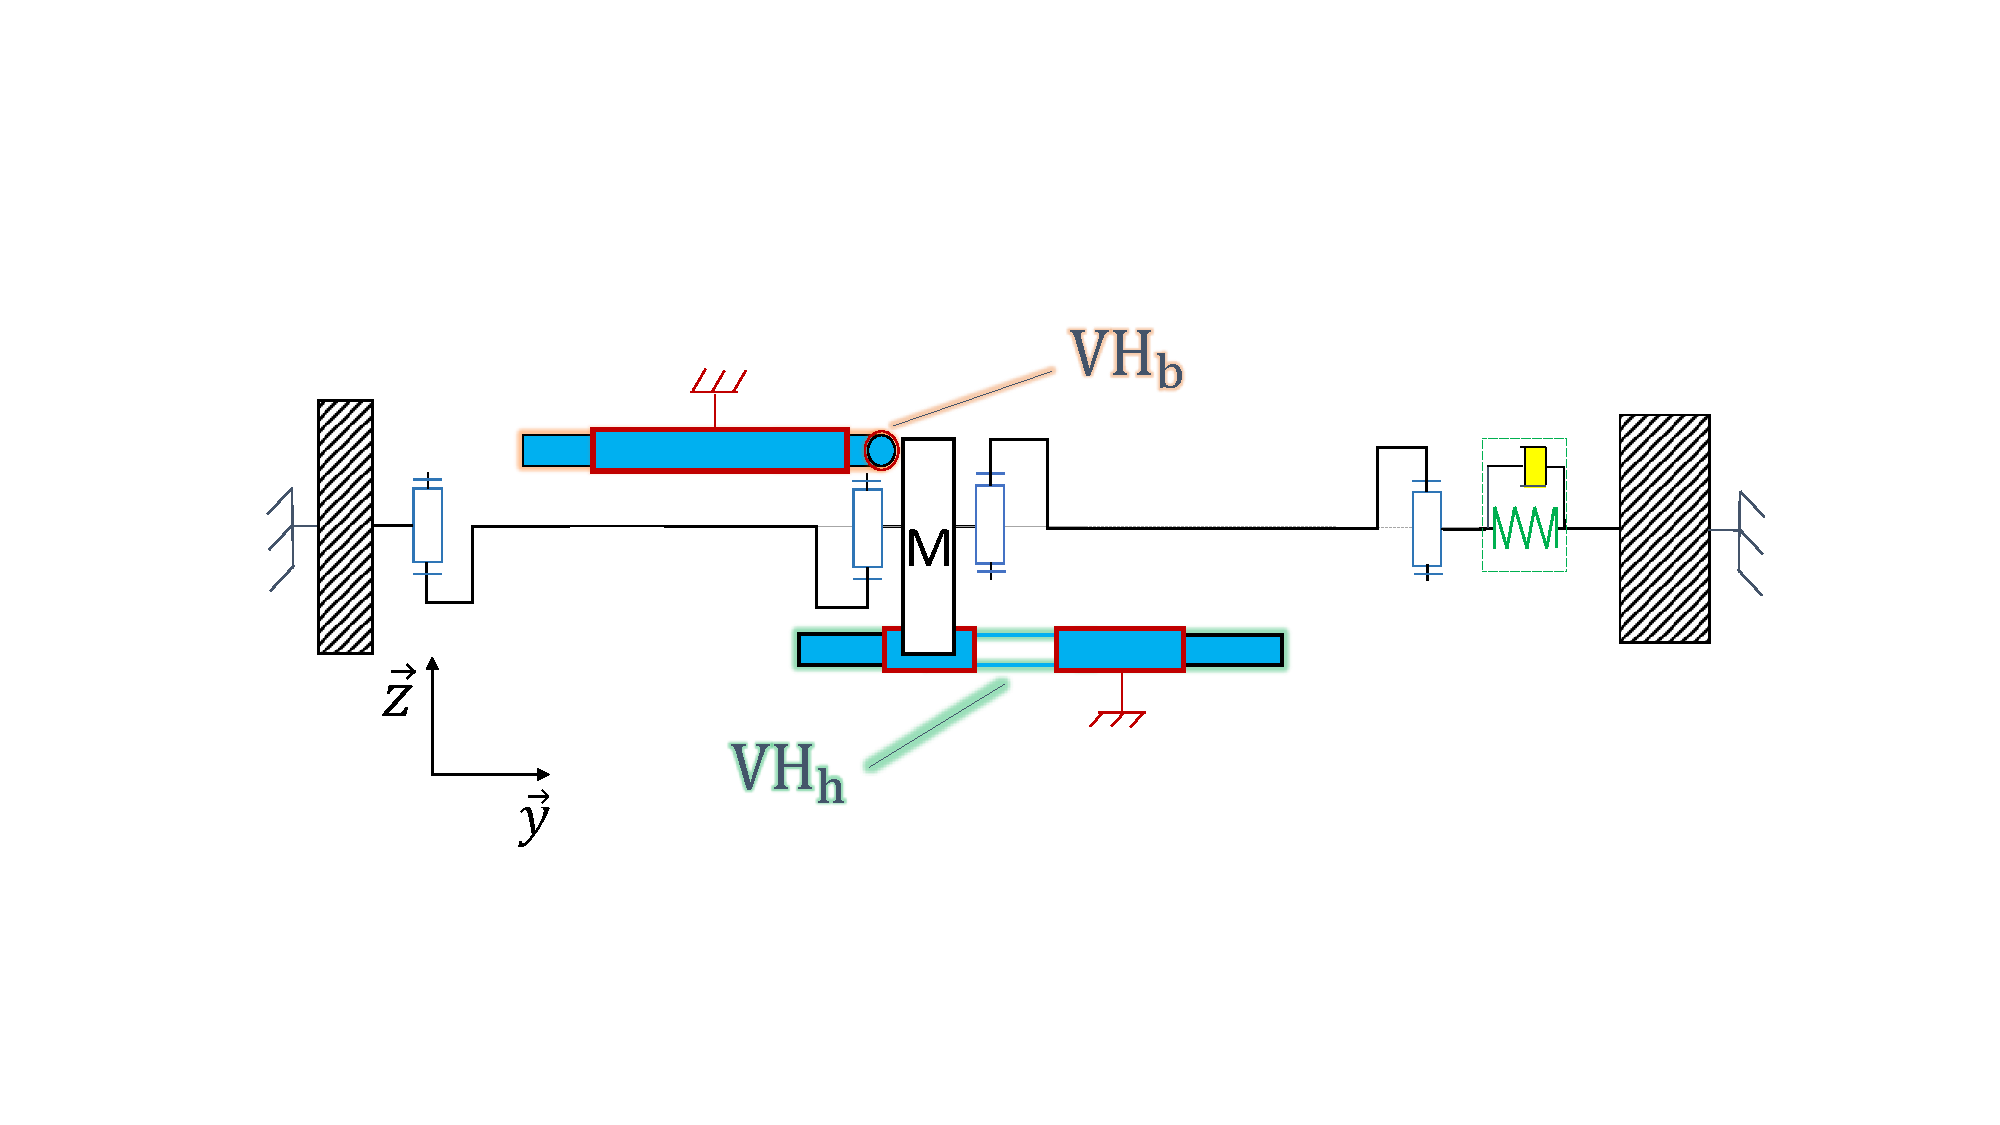
\includegraphics[trim={4cm 4.5cm 4cm 5cm},clip,width=0.8\textwidth]{../Chap2/Figure/integration_VH_dessus.pdf}
		\caption{Intégration VHs - Schéma cinématique vu dans la direction de l'axe des oscillations de M}
		\label{fig:integration_VH_dessus}
	\end{center}
\end{figure}
%%%%%%%%%%%%%%%%%%%%%%%%%%%%%

Par ailleurs, de nombreuses études mettent en avant le comportement non linéaire autour du phénomène de flambement des tubes en flexion post-flambement \cite{Corona1996,Houliara2006,Ju1992,Liu2008}. Sur la figure \ref{fig:flambement_tubes_Chen2016} on peut trouver les résultats de l'étude de Corona et al. sur le moment normalisé des tubes en flexion en fonction de l'angle de flexion imposé pour différents rapports épaisseur/rayon d'après trois différents modèles qu'on trouve dans la littérature. On constate alors que tous les modèles prédisent qu'après l'apparition du flambement le moment généré à la section flambée chute considérablement et on peut par conséquent en déduire que la raideur en rotation du tube en ce point diminue. Ce phénomène est positif pour notre application avec l'idée de minimiser l'influence mécanique des VHs.
%%%%%%%%%%%%%%%%%%%%%%%%%%%%%%%%%%%
\begin{figure}[!htbp]
\begin{center}
    \captionsetup{justification=centering}
	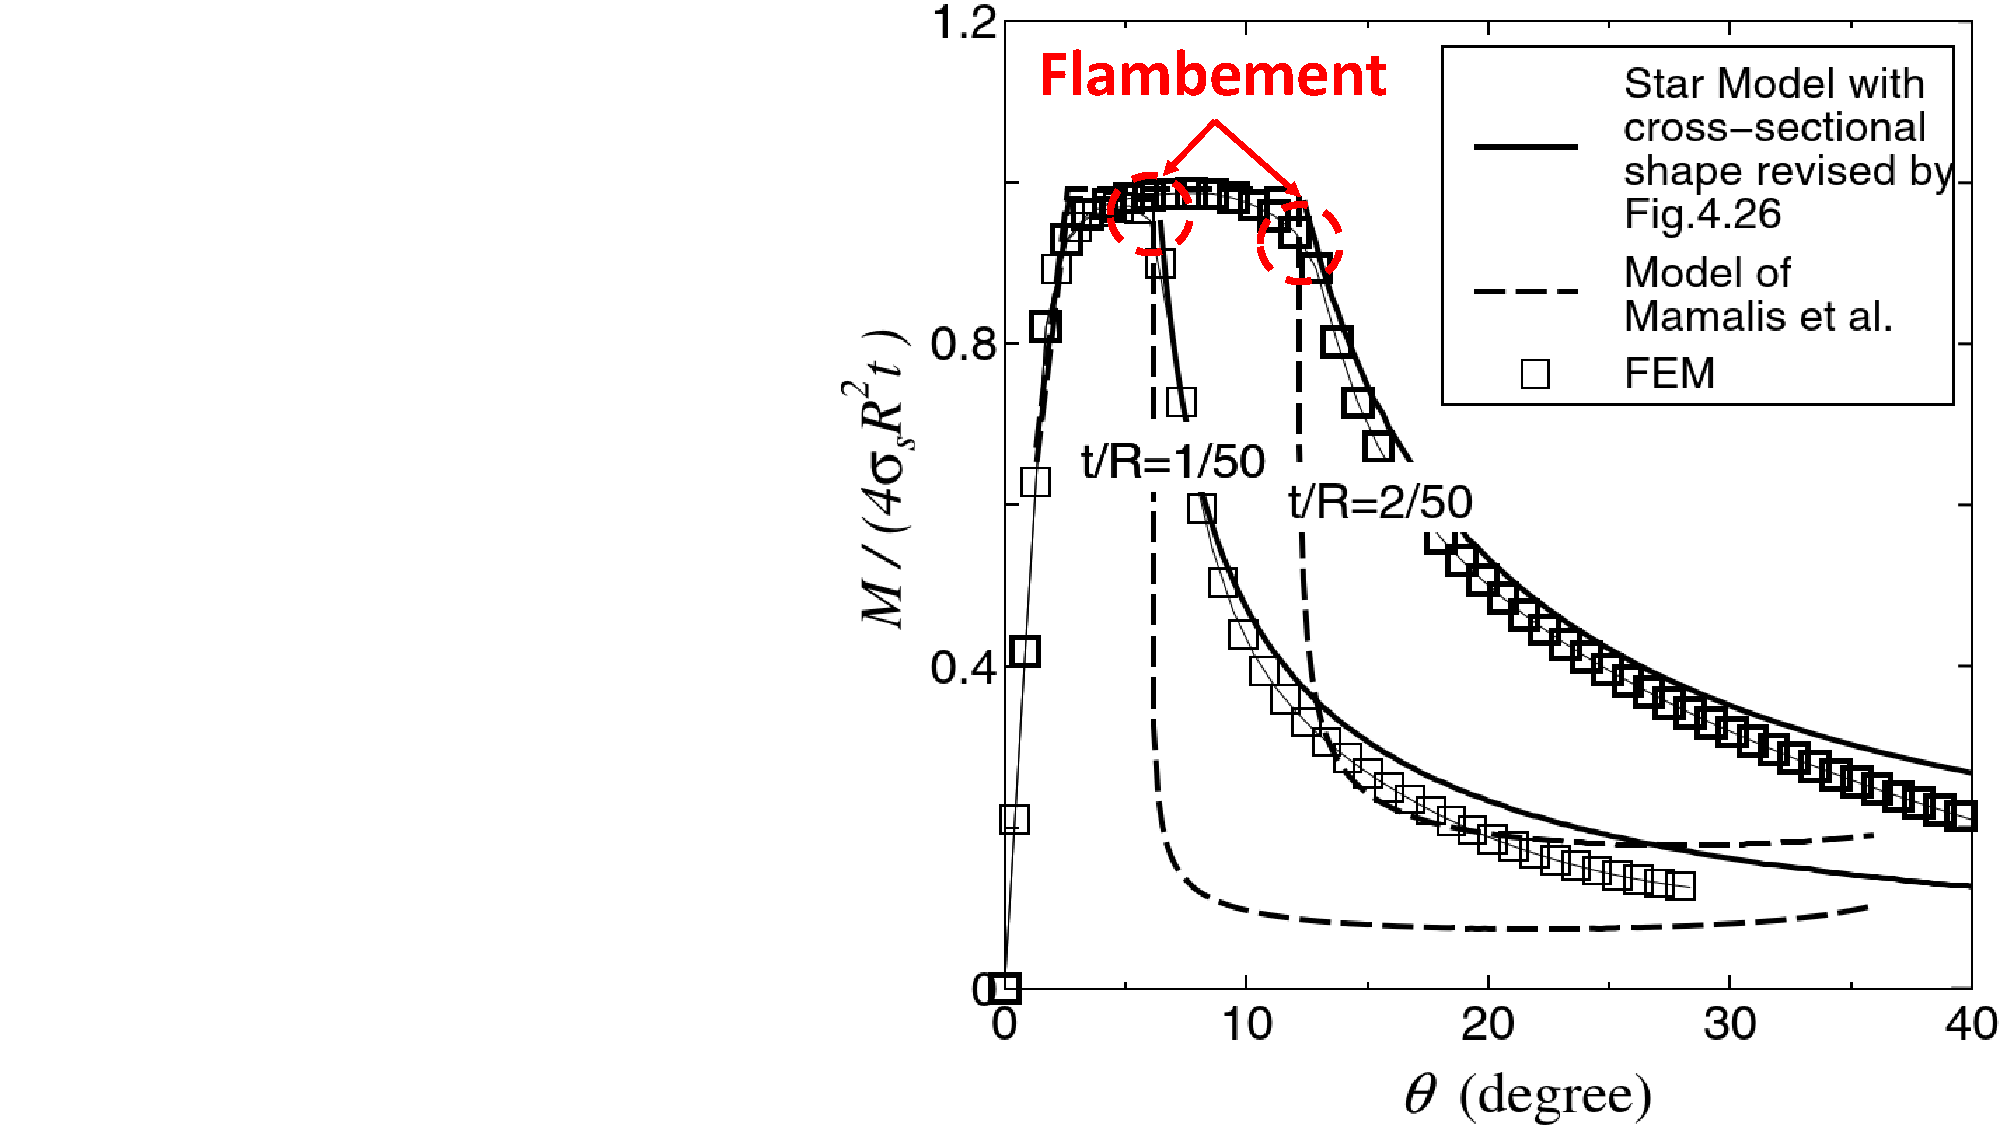
\includegraphics[trim={14cm 0cm 0cm 0cm},clip,width=0.5\textwidth]{../Chap2/Figure/flambement_tubes_Chen2016.pdf}
	\caption{Relation entre le moment et l'angle durant la sollicitation en flexion d'un cylindre creux \cite{Chen2016}}
	\label{fig:flambement_tubes_Chen2016}
\end{center}	
\end{figure}
%%%%%%%%%%%%%%%%%%%%%%%%%%%%%%%%%%%	
	
Cette solution technique amène deux types de dissipations énergétiques qui seront à minimiser une fois la preuve de concept démontrée. Ces-derniers sont le frottement de contact entre les deux composants M et VH et la dissipation du matériau du tube flexible.

Dans les deux prochaines sections, nous mettrons successivement en équation tous les composants du récupérateur d'énergie en mettant en évidence leur couplage.
%/!\/!\/!\/!\/!\/!\/!\/!\/!\/!\/!\/!\/!\/!\/!\/!\/!\/!\/!\/!\/!\/!\/!\/!\%
\section{Modélisation du convertisseur électromécanique}
\label{sec:2.3_Modélisation du convertisseur électromécanique}
%/!\/!\/!\/!\/!\/!\/!\/!\/!\/!\/!\/!\/!\/!\/!\/!\/!\/!\/!\/!\/!\/!\/!\/!\%
Dans cette section, nous allons mettre en équation le sous-système \emph{$SS_1$} composé de l'OB associé au GPA et d'un PH.\\
Le schéma cinématique du sous-système \emph{$SS_1$} est présenté sur la figure \ref{fig:schema_cinematique1}. Les paramètres du système  sont définis sur le schéma cinématique \ref{fig:schema_cinematique1} et dans le tableau \ref{tab:parametres}.

La structure nécessite un choix technologique pour réaliser les liaisons "pivot" aux centres de rotation A, A', B et B'. Une solution standard serait d'utiliser des roulements à billes ou à aiguilles. Cependant, ces solutions sont complexes à réaliser et intégrer à l'échelle de notre application. On propose de mettre en \oe{}uvre des liaisons souples qui seront dimensionnées dans le chapitre \ref{ch:3_Conception et fabrication du convertisseur electromecanique : OB + GPA}. Une telle solution se prête plus facilement à l'intégration sur un dispositif à l'échelle de l'oreille. De plus, elle s'affranchit de tout montage et d'éventuels jeux qui pourraient induire une baisse du coefficient de couplage. Cet aspect sera notable et discuté durant les caractérisations expérimentales du convertisseur électromagnétique..
%%%%%%%%%%%%%%%%%%%%%%%%%%%%%%%%%%%%
\begin{table}[!htbp]
	\centering
	\rowcolors[]{2}{black!8}{}{
		\begin{tabular}{m{0.7\textwidth}|c|c}
			\rowcolor{blue!10}
			\toprule
			Définition du paramètre                          & Symbole       & [Unité]    \\
			\midrule
			Masse                                            & $m$           & [kg]       \\
			Distance entre deux liaisons pivots adjacents    & $L$           & [m]        \\
			Niveau de flambement                            & $x_0$         & [m]        \\
			Raideur du GPA                                   & $K$           & [N/m]      \\
			Raideur en rotation d'une liaison pivot          & $K_{\varphi}$ & [Nm/rad]   \\
			Coefficient d'amortissement visqueux             & $\mu$         & [Pa.s]     \\
			Facteur de force du GPA                          & $\alpha$      & [N/V]      \\
			Capacité du GPA                                  & $C_0$         & [F]        \\
			Résistance de charge                             & $R_{ch}$      & [$\Omega$] \\
			Bras de levier de pliage de la VH par la masse M & $a$           & [m]        \\
			Raideur en rotation de la VH                     & $K_{VH}$      & [Nm/rad]   \\
			Coefficient de couplage électromécanique du GPA  & $k^2$         & [~~]       \\
			\bottomrule
		\end{tabular}}
	\caption{Définition des paramètres}
	\label{tab:parametres}
\end{table}
%%%%%%%%%%%%%%%%%%%%%%%%%%%%%%%%%%%%%%%%%%%%%%%%%%%%      
\begin{table}[!htbp]
	\begin{minipage}{0.5\textwidth}
		\centering
		\rowcolors[]{2}{black!8}{}{
			\begin{tabular}{c|c}
				\rowcolor{blue!10}
				\toprule
				\textbf{Numéro}  & \textbf{Nom}            \\
				\midrule
				0       & Bâti                             \\
				1 \& 1' & Bras de l'OB                     \\
				2       & M                                \\
				3       & Tête de piston                   \\
				4       & GPA                              \\
				5       & Modèle mécanique simplifié de VH \\
				\bottomrule
			\end{tabular}}
		\caption{Désignation des corps rigides}
		\label{tab:designation_pieces}
	\end{minipage}
	\hfillx
	\begin{minipage}{0.5\textwidth}
		\centering
		\rowcolors[]{2}{black!8}{}{
			\begin{tabular}{c|c}
				\rowcolor{blue!10}
				\toprule
				\textbf{Point}          & \textbf{Nature du point}        \\
				\midrule
				A \& A' \& B \& B' \& O & Centres des liaisons pivots     \\
				C \& T                  & Centre des liaisons ponctuelles \\
				G                       & Centre de gravité de M          \\
				\bottomrule
			\end{tabular}}
		\caption{Nature des points}
		\label{nature_points}
	\end{minipage}
\end{table}
%%%%%%%%%%%%%%%%%%%%%%%%%%%%%%%%%%%%%%%%%
\begin{figure}[!htbp]
	\begin{center}
		\captionsetup{justification=centering}
		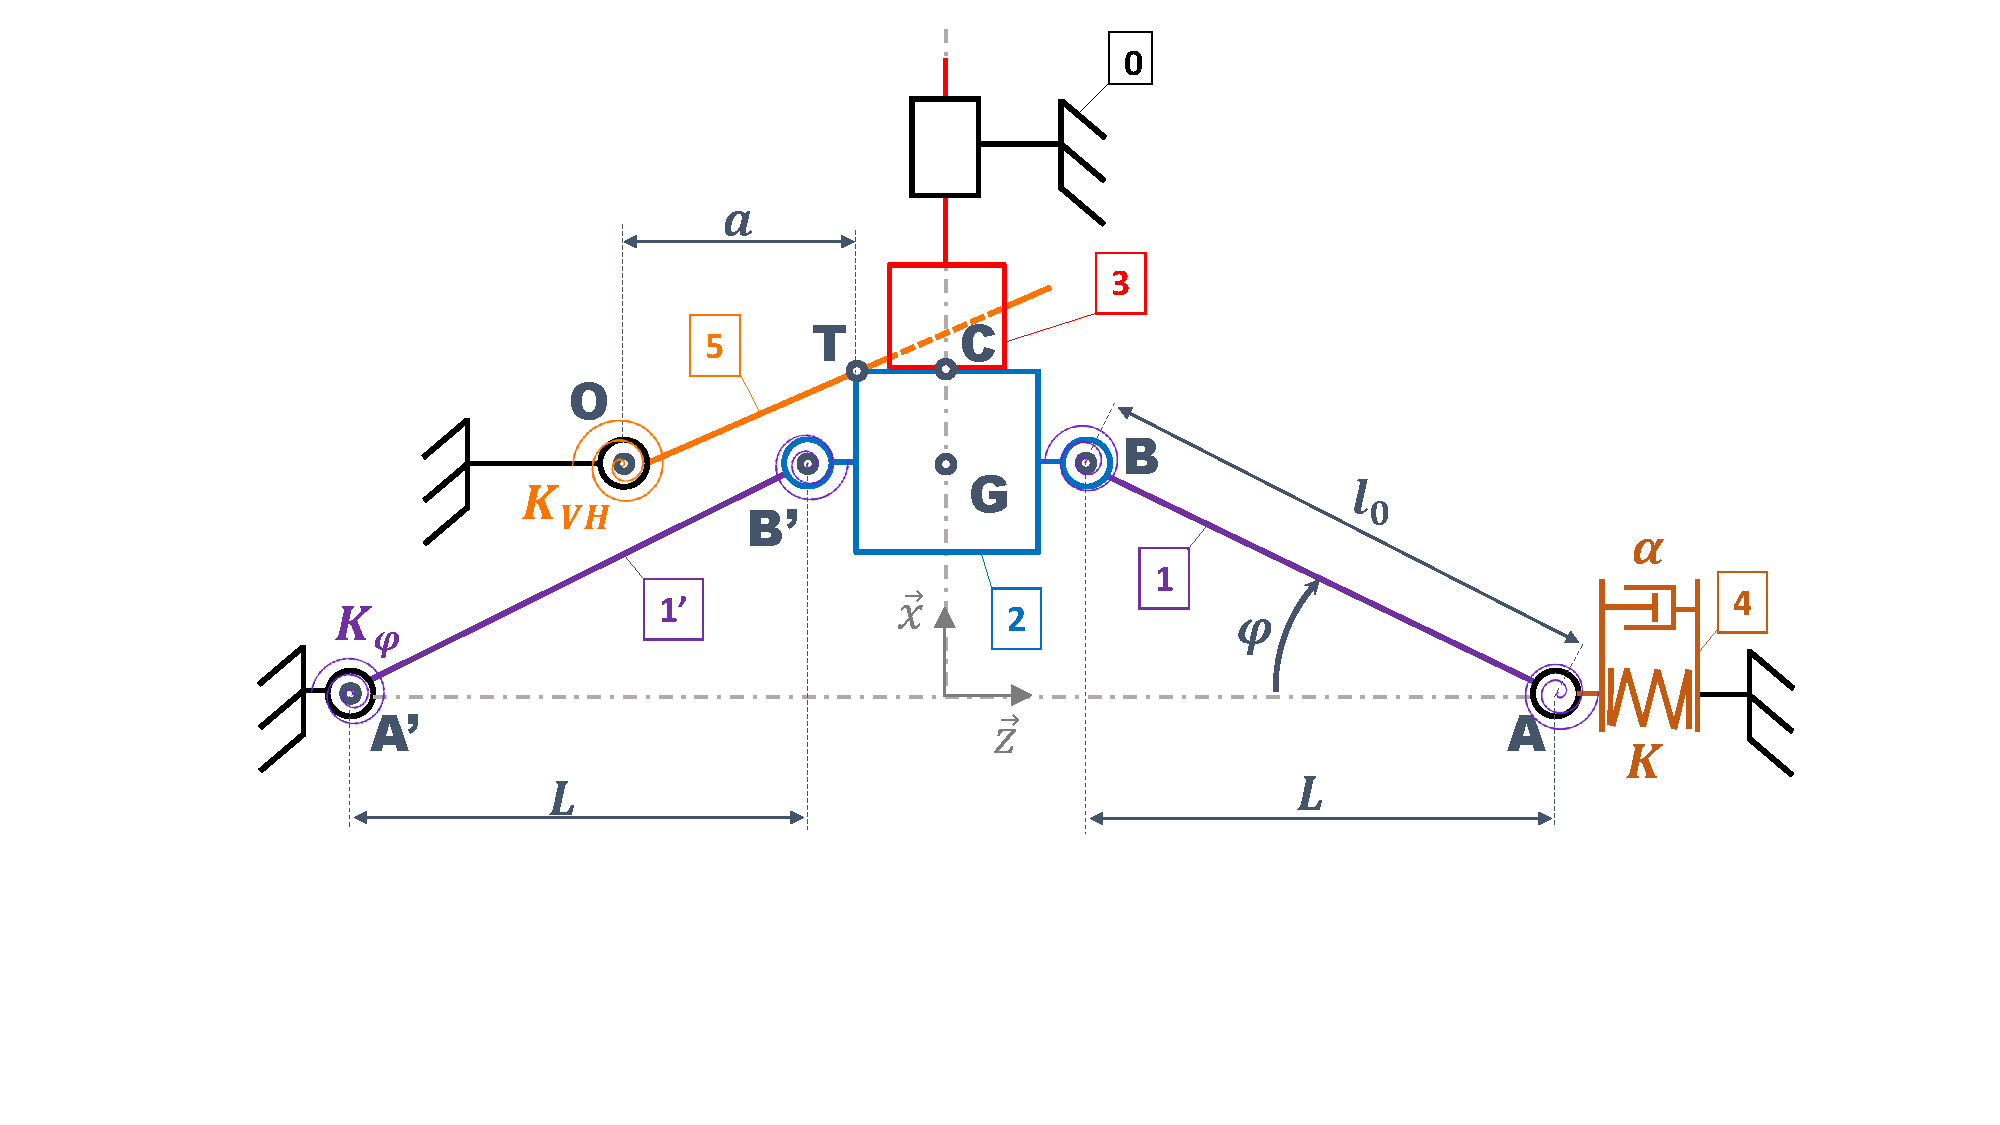
\includegraphics[trim={4cm 5cm 3cm 0cm},clip,width=\textwidth]{../Chap2/Figure/schema_cinematique1.pdf}
		\caption{Schéma cinématique }
		\label{fig:schema_cinematique1}
	\end{center}
\end{figure}
%%%%%%%%%%%%%%%%%%%%%%%%%%%%%%%%%%%%%%%%%

Les hypothèses de la modélisation sont les suivantes :
\begin{itemize}[label=$\circ$]
	\item Le corps isolé est M (pièce 2).
	\item Toutes les pièces sont supposées infiniment rigides, mis à part le GPA (pièce 4) qui possède une raideur $K$, ainsi qu'un coefficient de couplage électromécanique $k^2$ traduisant la transduction piézoélectrique et défini par l'équation \ref{eq:k2_definition_APA}.
	\item Les masses des composants périphériques à la pièce 2 sont négligées.
	\item Les liaisons pivots aux points A, B, A' et B' seront supposées élastiques. Elles seront définies par leur raideur en rotation $K_{\varphi}$. Leur dissipation structurelle est incluse dans le coefficient d'amortissement visqueux global $\mu$.
	\item Le contact entre M et VH (pièce 5) est ponctuel au point T. Les deux pièces sont supposées en contact permanent durant les oscillations de M.
	\item Quand la précontrainte de flambement appliquée sur l'axe $\vec{z}$ de l'OB est nulle, la masse se trouve en $x=0$. On notera alors $l_0$ la longueur entre deux pivots adjacents dans ce cas précis.
	\item L'étude sera limitée par l'hypothèse de petits angles ${\varphi}$ en supposant que $x_0<<L$.
\end{itemize}
\begin{equation}
	k^2 = \dfrac{\alpha^2 }{\alpha^2 + KC_0}
	\label{eq:k2_definition_APA}
\end{equation}
	%////////////////////////////////////////////
	\subsection{Modèle OB + GPA}
	\label{2.3.1_Modèle OB + GPA}
	%////////////////////////////////////////////
Considérons dans un premier temps l'OB seul avec le GPA, sans tenir compte de l'impact du piston et de la VH. En isolant M et en appliquant le principe fondamental de la dynamique projeté suivant l'axe $\vec{x}$, on obtient l'équation suivante :
\begin{equation}
m \ddot{x}_m = - 2K(\sqrt{x_m^2+L^2}-l_0)\tan(\varphi) - \mu \dot{x}_m			
			 - \frac{4K_{\varphi}\varphi}{L}
			 - 2\alpha U_p \tan(\varphi)
\label{eq:OB-GPA}
\end{equation}
Où $U_p$ est la tension aux bornes du GPA. Le circuit d'extraction d'énergie va générer une extraction d'énergie électrique. L'équation régissant le comportement électrique du GPA est :
\begin{equation}
	\dfrac{U_p}{R_{ch}} = 
	-\alpha\dfrac{d}{dt}\biggl(2\sqrt{{l_0}^2-x_m^2}\biggr)
	- C_0\dot{U_p}
	= \frac{2\alpha x_m\dot{x}_m}{\sqrt{L^2+x_m^2}} - C_0\dot{U_p}
\end{equation}
$R_{ch}$ est la résistance d'entrée du circuit d'extraction d'énergie. Par conséquent, la puissance récupérable $P_{e}$ peut s'exprimer par :
\begin{equation}
P_e = \frac{{U_p}^2}{R_{ch}} 
\label{eq:P_e}
\end{equation} 

Le niveau de flambement $\epsilon$ de l'OB est défini comme le rapport de la position d'équilibre $x_0$ sur la longueur $L$. Plus le niveau de flambement est élevé et plus la force nécessaire pour faire basculer M d'une position stable vers l'autre est importante. Dans les conditions de petits angles $\varphi$, le système d'équations électromécaniques couplées \ref{eq:OB-GPA_linear} définit le comportement de l'OB intégrant le GPA.
\begin{equation}
\begin{dcases}
\ddot{x}_m = - \Biggl[ \frac{2K}{mL^2}( x_m^2+L^2 -{l_0}^2) + \frac{4K_{\varphi}}{mL^2} \Biggr]x_m
	- \biggl( \frac{\mu}{m} \biggr) \dot{x}_m
	- \frac{2\alpha U_p\ x_m}{mL} \\
\dfrac{U_p}{R_{ch}} = \frac{2\alpha x_m \dot{x}_m}{L} - C_0\dot{U}_p
\end{dcases}
\label{eq:OB-GPA_linear}
\end{equation}
Les positions d'équilibre stables $\pm x_0$ peuvent alors s'exprimer par l'équation \ref{eq:x0}.
\begin{equation}
x_0 = \pm \sqrt{{l_0}^2-L^2-\frac{4K_{\varphi}}{K}}
\label{eq:x0}
\end{equation}


La bistabilité de l'oscillateur dépend alors du rapport entre la raideur des liaisons pivots et celle du GPA, pour un niveau de flambement donné. Il existe donc une limite pour $K_{\varphi}$, exprimée par l'équation \ref{eq:K_phi_lim}, au-delà de laquelle l'oscillateur n'admet qu'une seule position stable en $x=0$.
\begin{equation}
K_{\varphi} < \frac{(l_0^2-L^2)K}{4}
\label{eq:K_phi_lim}
\end{equation}

L'influence de la rigidité des liaisons pivots sur l'énergie potentielle élastique, ainsi que sur la force élastique de l'OB est illustré sur la figure \ref{fig:impact_Kphi}.
%%%%%%%%%%%%%%%%%%%%%%%%%
\begin{figure}[!htbp]
\begin{center}
	\begin{subfigure}[b]{0.4\textwidth}
    	\captionsetup{justification=centering}
		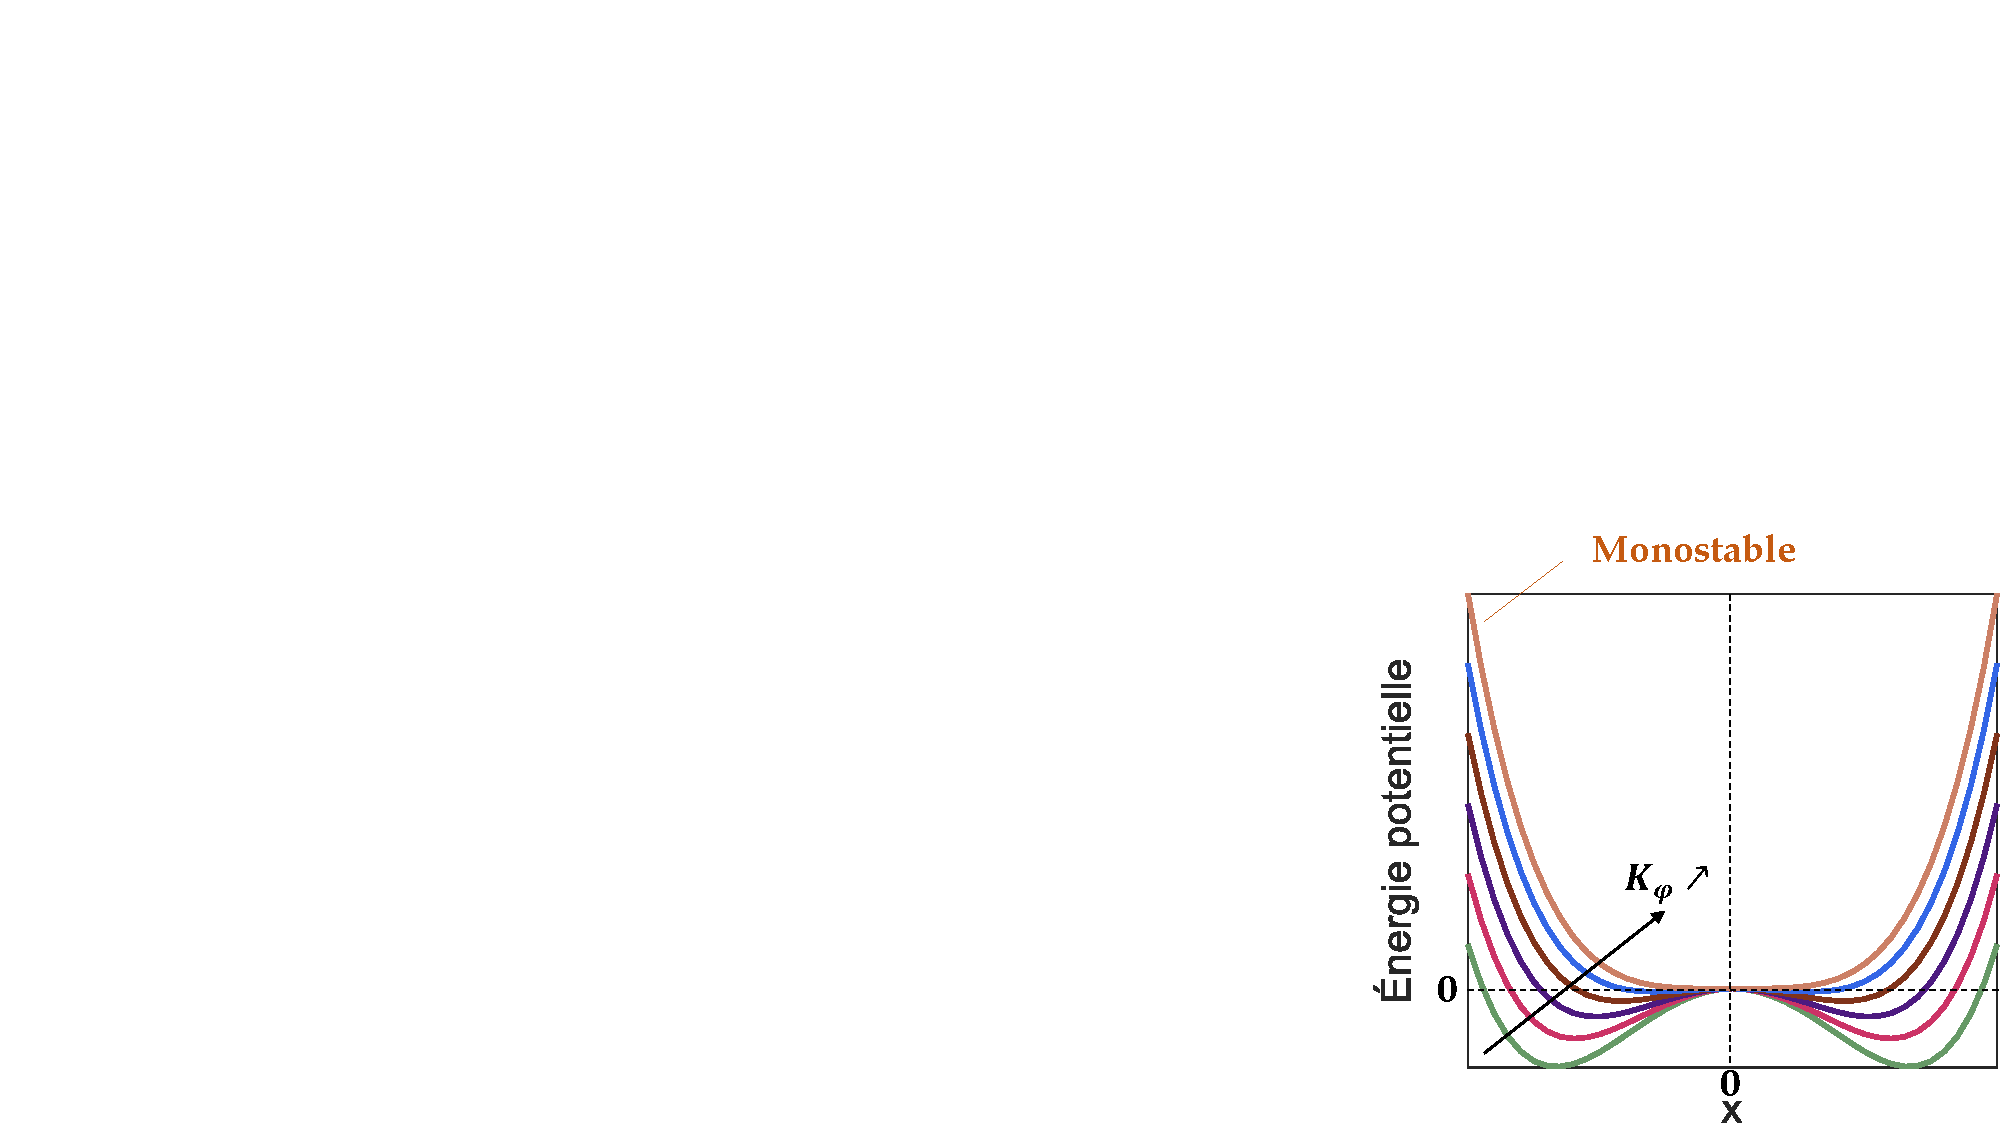
\includegraphics[trim={23cm 0cm 0cm 9cm},clip,width=\textwidth]{../Chap2/Figure/Kphi_Ep.pdf}
		\caption{Impact de $K_{\varphi}$ sur l'énergie potentielle}
		\label{fig:Kphi_Ep}
	\end{subfigure}
\hfillx
	\begin{subfigure}[b]{0.38\textwidth}
    	\captionsetup{justification=centering}
		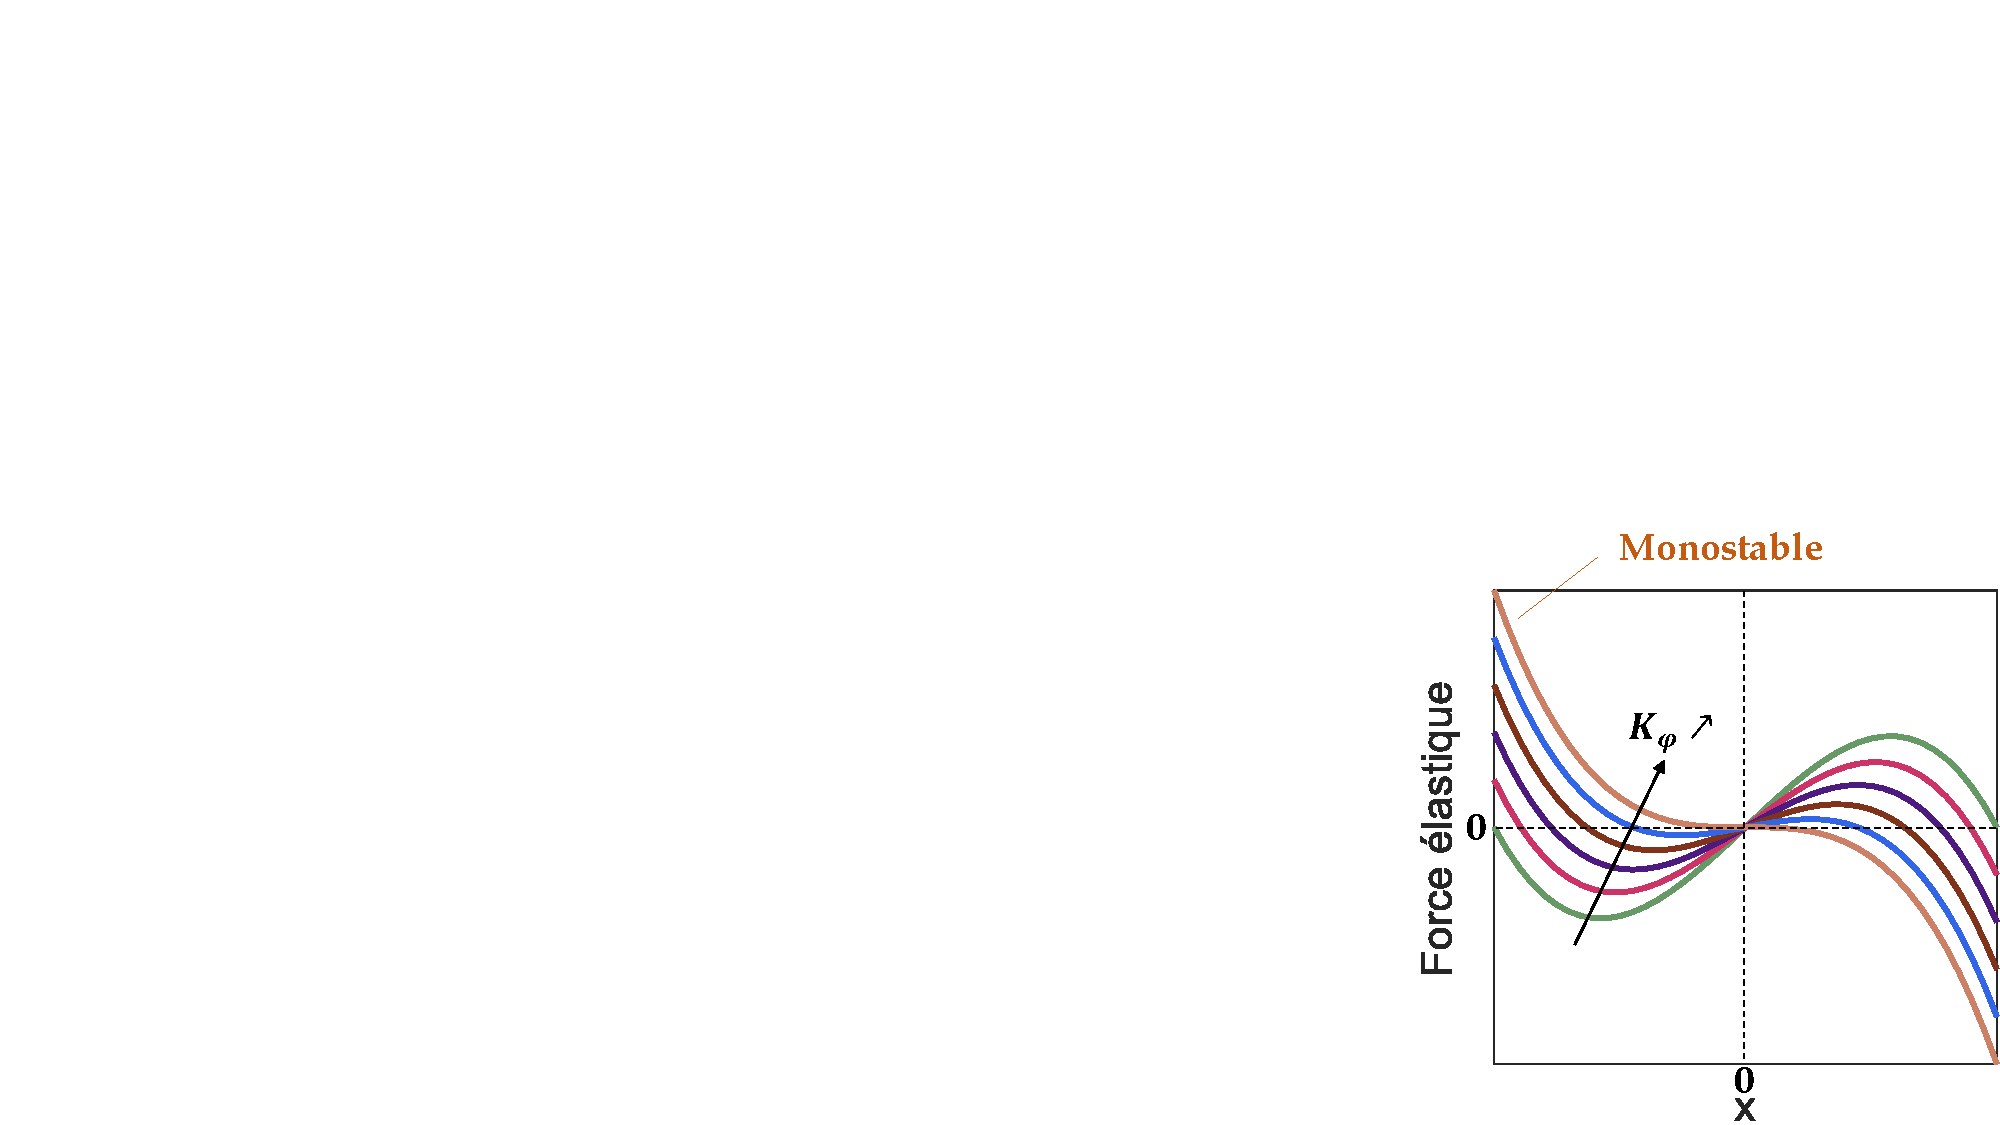
\includegraphics[trim={24cm 0cm 0cm 9cm},clip,width=\textwidth]{../Chap2/Figure/Kphi_Felas.pdf}
		\caption{Impact de $K_{\varphi}$ sur la force élastique}
		\label{fig:Kphi_Felas}  
	\end{subfigure}
	\caption{Impact de $K_{\varphi}$ sur le comportement mécanique de l'OB}
	\label{fig:impact_Kphi}
\end{center}	
\end{figure}
%%%%%%%%%%%%%%%%

En réarrangeant les termes de l'équation \ref{eq:OB-GPA_linear} de façon à faire apparaître la position d'équilibre stable, on obtient:
\begin{equation}
\begin{dcases}
\ddot{x} = - \frac{2K{x_0}^2}{mL^2}\biggl(\frac{x_m^2}{{x_0}^2} -1\biggr)x_m
	- \biggl( \frac{\mu}{m} \biggr) \dot{x}_m
	- \frac{2\alpha U_p\ x_m}{mL} \\
\dfrac{U_p}{R_{ch}} = \frac{2\alpha x_m \dot{x}_m}{L} - C_0\dot{U}_p
\end{dcases}
\label{eq:OB-GPA_linear_canonique}
\end{equation}
Le comportement mécanique de l'OB pour des faibles niveaux de flambement $\epsilon$ est régi par l'équation de Duffing en régime libre \cite{Huguet2019} :
\begin{equation}
\ddot{x}  
+ \frac{{\omega_0}^2}{2}\biggl( \frac{x_m^2}{{x_0}^2} - 1 \biggr)x_m
+ \biggl(\frac{\omega_0}{Q}\biggr)\dot{x}_m
= 0
\label{eq:Duffing}
\end{equation}
On peut alors par identification avec les équations \ref{eq:OB-GPA_linear_canonique} et \ref{eq:Duffing}, définir le facteur de qualité mécanique $Q$ de l'OB ainsi que la pulsation propre $\omega_0$ comme :
\begin{equation}
 \begin{dcases}
\omega_0 = \frac{x_0}{L}\sqrt{\frac{2K}{m}} \\
Q = \frac{x_0}{L}\frac{\sqrt{{2Km}}}{\mu}
 \end{dcases}
\label{eq:w0_Q}
\end{equation}
	%////////////////////////////////////////////
	\subsection{Influence de l'actionnement hydraulique sur le modèle OB + GPA}
	\label{2.3.2_Influence du circuit hydraulique sur le modele OB-GPA}
	%////////////////////////////////////////////	
On considère maintenant que M est en contact avec le PH, ainsi qu'avec la VH. La valve possède une raideur en rotation et le piston génère une force $F_{pis}$. Dans ces conditions, l'équilibre dynamique de M est donné par l'équation \ref{eq:OB+GPA+VH+piston}.
\begin{equation}
\begin{small}
\begin{dcases}
\ddot{x}_m = - \frac{2K{x_0}^2}{mL^2}\biggl(\frac{x_m^2}{{x_0}^2} -1\biggr)x_m - \frac{\mu}{m}\dot{x}_m - \frac{2\alpha U_p\ x_m}{mL} - \underbrace{\frac{K_{VH}(x_m)\theta(x_m)}{ma} - \frac{F_f\sign(\dot{x}_m)}{m}}_{VH} - \overbrace{\frac{F_{pis}}{m} }^{Piston}\\
\dfrac{U_p}{R_{ch}} = \frac{2\alpha x_m \dot{x}_m}{L} - C_0\dot{U}_p
\end{dcases}
\label{eq:OB+GPA+VH+piston}	
\end{small}
\end{equation}
$F_{pis}$ correspond à la poussée QS générée par le piston afin de faire basculer M vers la position stable opposée. Elle est définie à l'équation \ref{eq:F_pis} par la force hydraulique disponible dans la branche qui actionne. 
\begin{equation}
	F_{pis} = \dfrac{p_p}{S_p}
	\label{eq:F_pis}
\end{equation}
Avec $p_p$ et $S_p$ qui correspondent respectivement à la pression dans la chambre du piston actif et à la section de ce dernier. La barrière de potentiel énergétique à franchir par M, si $K_{VH}$ est négligeable, peut par ailleurs s'exprimer avec l'équation \ref{eq:Barriere energie potentielle OB}. 
\begin{equation}
	Ep_{bar} = \dfrac{K{x_0}^4}{2L^2}
	\label{eq:Barriere energie potentielle OB}
\end{equation}
L'influence de $K_{VH}$ sur la barrière de potentiel de l'OB sera discuté dans le chapitre \ref{ch:6_Comportement du systeme de recuperation d’energie intra-auriculaire avec les composants caracterises experimentalement}.

Le second terme amené par la VH dans l'équation \ref{eq:OB+GPA+VH+piston} traduit les frottements secs au contact M-VH lors de la phase d'oscillations. Ces frottements, négligés dans un premier temps pour un pré-dimensionnement, seront déterminés expérimentalement dans le chapitre \ref{ch:6_Comportement du systeme de recuperation d’energie intra-auriculaire avec les composants caracterises experimentalement}. De la même façon que $K_{\varphi}$, $K_{VH}$ affecte le comportement mécanique de l'OB. Cet aspect est discuté dans le chapitre \ref{ch:6_Comportement du systeme de recuperation d’energie intra-auriculaire avec les composants caracterises experimentalement} lors de l'intégration des données expérimentales des valves dans le modèle global.
%/!\/!\/!\/!\/!\/!\/!\/!\/!\/!\/!\/!\/!\/!\/!\/!\/!\/!\/!\/!\/!\/!\/!\/!\%
\section{Modélisation du circuit hydraulique}
\label{sec:2.4_Modelisation du circuit hydraulique}
%/!\/!\/!\/!\/!\/!\/!\/!\/!\/!\/!\/!\/!\/!\/!\/!\/!\/!\/!\/!\/!\/!\/!\/!\%
Dans cette section nous allons nous intéresser au circuit hydraulique composé du bouchon d'oreille, des deux valves, des deux pistons, des deux clapets anti-retour, ainsi que de l'AH. 
		%////////////////////////////////////////////
		\subsection{Expression des pertes de charges dans une VH}
		\label{sec:2.4.1_Expression des pertes de charges dans une VH}
		%////////////////////////////////////////////
Il existe deux types de pertes de charges (PdC). Les PdC régulières et les PdC singulières. Les PdC régulières correspondent à la perte de pression générée par le frottement du fluide sur les parois d'une conduite à section régulière lors d'un écoulement. Les PdC singulières, quant à elles, correspondent à la perte de pression générée au passage du fluide à travers toute modification géométrique brutale d'une conduite. Au passage des VHs, l'écoulement du fluide est donc soumis à des PdC singulières. Avec $p_1$ la pression en entrée d'une perturbation géométrique et $p_2$ la pression en sortie, les pertes de charges $\Delta p$ s'expriment par l'équation \ref{eq:PdC_sing_vitesse} \cite{Idelcik1986}.
\begin{equation}
\Delta p = p_1 - p_2 = \Lambda \biggl(\frac{{\rho} v^2}{2}\biggr)\\
\label{eq:PdC_sing_vitesse}
\end{equation}
$v$ : Vitesse moyenne d'écoulement du fluide [$m/s$]\\
$\Lambda$ : Coefficient de pertes de charges singulières\\

Le coefficient $\Lambda$ est généralement déterminé de manière empirique et référencé dans des abaques \cite{Idelcik1986,Giles2013}.

Dans la suite de l'étude, nous allons travailler avec les niveaux de débits issus du bouchon d'oreille (fig.  \ref{fig:debit_ear}) \cite{Delnavaz2012}. L'équation \ref{eq:PdC_sing_vitesse} peut alors être exprimée par \ref{eq:PdC_sing_debit}.
\begin{equation}
\Delta p =  \biggl(\frac{8\rho}{\pi {D_h}^4}\biggr)\Lambda q^2
\label{eq:PdC_sing_debit}
\end{equation}
Où $D_h$ est le diamètre hydraulique de la section de passage. Ce diamètre est utilisé pour caractériser un écoulement au travers de conduites à section non circulaire. Il est défini comme le diamètre équivalent de la conduite à section circulaire qui générerait les mêmes pertes de charges que la section de passage étudiée \cite{Brater1988}. Il s'exprime comme suit :
\begin{equation}
D_h = \frac{4S}{\mathcal{P}}
\label{eq:Dh_definition}
\end{equation}
Où $S$ est la section de passage et $\mathcal{P}$ le périmètre de cette section. Pour simplifier l'écriture, on définit le coefficient de pertes de charges $Cf$, exprimé en [Pa.s$^2$m$^{-6}$], comme étant le rapport des pertes de charges singulières sur le carré du débit. Ainsi on a :
\begin{equation}
Cf = \frac{\Delta p}{q^2} = \biggl(\frac{8\rho}{\pi {D_h}^4}\biggr)\Lambda
\label{eq:Cf_definition}
\end{equation}
Sachant que la fermeture des VHs sera gouvernée par la position de M, $Cf$ sera une fonction de $x$. Par ailleurs le comportement des VHs doit être symétrique par rapport à la position $x_m=0$. $Cf$ est donc une fonction paire par rapport à $x$ : $Cf(x) = Cf(-x)$. De plus, on notera $Cf_0$ la valeur du coefficient de pertes de charges lorsque la masse M n'est pas en contact avec la VH.
		%////////////////////////////////////////////
		\subsection{Mise en équation}
		\label{sec:2.4.2_Mise en équation}		
		%////////////////////////////////////////////
Le schéma hydraulique de la figure \ref{fig:schema_hydraulique_global} montre le couplage hydromécanique depuis le bouchon d'oreille jusqu'aux PHs. Les indices \emph{h} et \emph{b} font respectivement référence aux branches \emph{haut} et \emph{bas} introduites plus tôt lors de la présentation globale du système (sec. \ref{subsec:2.1.2_Presentation du systeme complet}). Le pilotage de l'ouverture/fermeture des VHs est assuré par la position de M suivant le cycle détaillé dans le tableau \ref{tbl:act_top}. Le clapet anti-retour assurant le retour de fluide dans le bouchon d'oreille pour une valve en position fermée. Les paramètres hydrauliques sont référencés dans le tableau \ref{tab:parametres_hyd}.
%%%%%%%%%%%%%%%%%%%%%%%%%%%%%%%%%%%%%%%%%
\begin{figure}[!htbp]
	\begin{center}
		\captionsetup{justification=centering}
		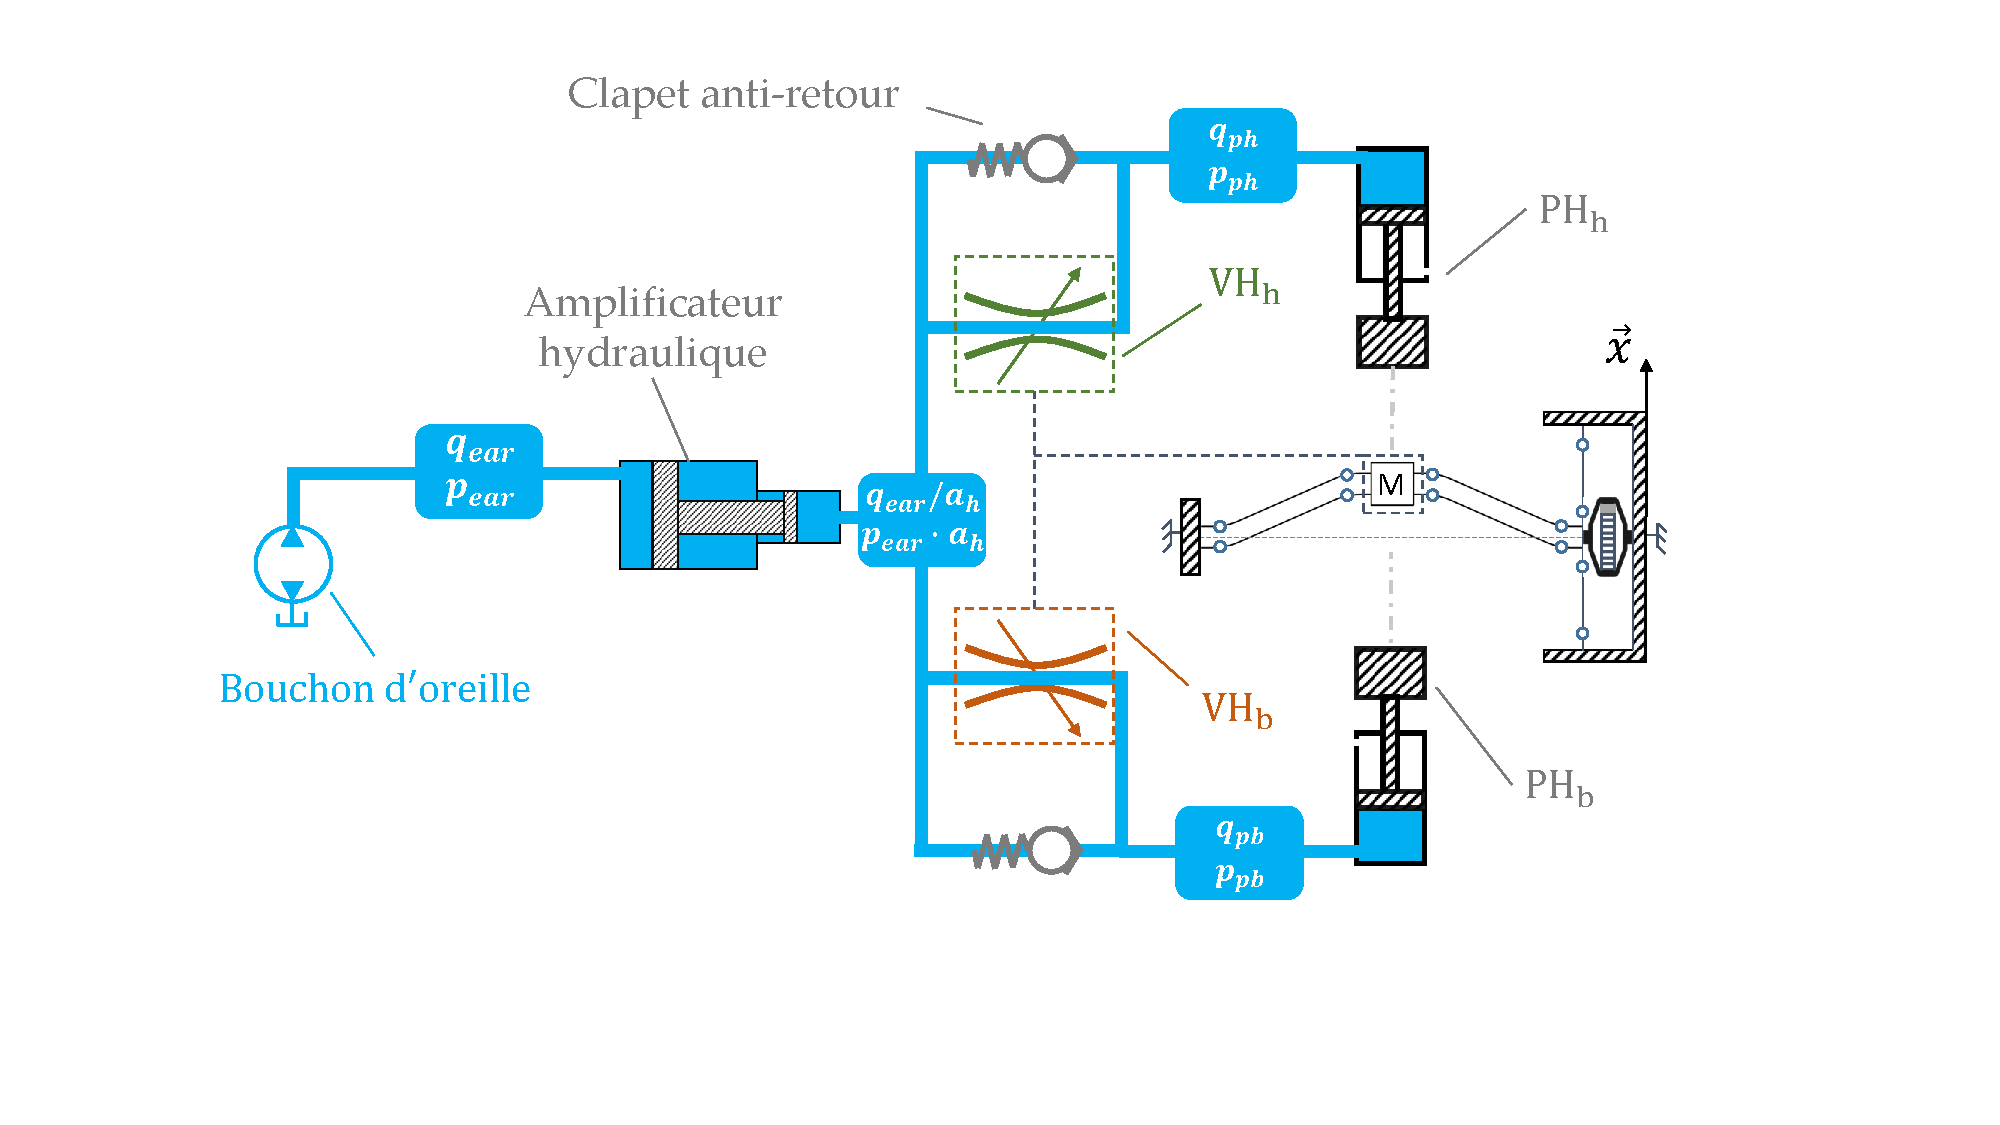
\includegraphics[trim={3.5cm 3.5cm 5.5cm 1cm},clip,width=0.8\textwidth]{../Chap2/Figure/schema_hydraulique2.pdf}
		\caption{Schéma hydraulique global}
		\label{fig:schema_hydraulique_global}
	\end{center}
\end{figure}
%%%%%%%%%%%%%%%%%%%%%%%%%%%%%%%%%%%%%%%%%
%%%%%%%%%%%%%%%%%%%%%%%%%%%%%%%%%%%%
\begin{table}[!htbp]
	\centering
	\rowcolors[]{2}{black!8}{}{
		\begin{tabular}{m{0.7\textwidth}|c|c}
			\rowcolor{blue!10}
			\toprule
			\textbf{Définition du paramètre}             & \textbf{Symbole} & \textbf{[Unité]} \\
			\midrule
			Coefficient de PdC de VH ouverte             & $Cf_0$           & [$Pa.s^2m^{-6}$] \\
			Coefficient de frottement visqueux du piston & $C_p$            & [$Ns.m^{-1}$]    \\
			Section du piston                            & $S_p$            & [$m^2$]          \\
			Pression de gonflage du bouchon d'oreille    & $p_{gon}$        & [$Pa$]           \\
			Coefficient d'amplification de pression      & $a_h$            & [~]              \\
			\bottomrule
		\end{tabular}}
	\caption{Définition des paramètres}
	\label{tab:parametres_hyd}
\end{table}
%%%%%%%%%%%%%%%%%%%%%%%%%%%%%%%%
			%*************
			\subsubsection{Équilibre dynamique du PH}
			\label{sec:2.4.2.a_Mise en equation}
			%*************
Afin de modéliser le comportement couplé des deux branches hydrauliques, on utilisera l'indice $"o"$ pour le circuit ouvert et l'indice $"f"$ pour le circuit fermé. Les hypothèses du modèle sont les suivantes :
\begin{itemize}[label=$\circ$]
	\item Le fluide est incompressible et Newtonien.
	\item Les conduites sont non déformables (pas de variation de volume).
	\item Le circuit hydraulique n'admet aucune fuite.
	\item L’actionnement hydraulique est considéré quasi-statique (QS) devant la fréquence oscillation de l’OB.
\end{itemize} 

En considérant les hypothèses énoncées ci-dessus, la projection suivant l'axe $\vec{x}$ du principe fondamental de la statique, appliqué aux pistons respectifs, donne les équations d'équilibre \ref{eq:equilibre_dynamique_piston_ouvert} et \ref{eq:equilibre_dynamique_piston_ferme}.
\begin{align}
\text{Piston ouvert~}& \left\{~
-F_{pis} - p_{po}\ S_{p} - C_{p}\ \dot{x}_{po} = 0
\right.
\label{eq:equilibre_dynamique_piston_ouvert}\\
\text{Piston fermé~}& \left\{~
p_{pf}\ S_{p} - C_{p}\ \dot{x}_{pf} = 0
\right.
\label{eq:equilibre_dynamique_piston_ferme}
\end{align}
Où $p_{p}$ est la pression dans la chambre du piston considéré et $x_p$ sa position. La force $-F_{pis}$ traduit la contre-réaction de M sur le PH. Elle s'exprime donc par l'équation \ref{eq:F_OB_xxxxxx}, tant que le contact entre le piston et M est maintenu.
\begin{equation}
-F_{pis} = F_{ob} = -\frac{K\ {x_0}^2}{L^2}\biggl(\frac{x_m^2}{{x_0}^2} -1\biggr)x_m - \biggl( \frac{K_{VH}}{a} \biggr) \arctan \biggl(\frac{x_m}{a} \biggr) - F_f\ \sign(\dot{x}_m)
\label{eq:F_OB_xxxxxx}
\end{equation}
Ce terme est donc obligatoirement nul pour l'équation d'équilibre dynamique du piston qui n'est pas en contact avec M.
			%*************
			\subsubsection{Équilibre hydraulique}
			\label{sec:2.4.2.b_Mise en équation}
			%*************
De même que pour l'équation d'équilibre mécanique, l'équilibre hydraulique sera régi par deux équations couplées. En nous appuyant sur le théorème de Bernoulli appliqué d'une part avant et d'autre part après l'AH, on peut établir les équations \ref{eq:equilibre_hydraulique_piston_ouvert} et \ref{eq:equilibre_hydraulique_piston_ferme} définissant le comportement des deux branches hydrauliques.
\begin{align}
\text{Branche ouverte~}& \left\{~
p_{ear} = p_{gon} + \frac{1}{a_h} \biggl( p_{po} +
		 \dfrac{\Delta p_{cl}(\text{sign}(q_{ear}))\cdot Cf_0\ {q_o}^2}{\Delta p_{cl}(\text{sign}(q_{ear}))\ +\ Cf_0\ {q_o}^2} \bigg)
\right.
\label{eq:equilibre_hydraulique_piston_ouvert}\\
\text{Branche fermée~}& \left\{~
p_{ear} = p_{gon} + \frac{1}{a_h} \biggl( p_{pf} +
 		\dfrac{\Delta p_{cl}(\text{sign}(q_{ear}))\cdot Cf(x_m)\ {q_f}^2}{\Delta p_{cl}(\text{sign}(q_{ear}))\ +\ Cf(x_m)\ {q_f}^2} \bigg)
\right.
\label{eq:equilibre_hydraulique_piston_ferme}
\end{align}
$\Delta p_{cl}$ traduit les PdC dans un clapet anti-retour et est fonction du signe du débit sortant/entrant du point de vue des pistons. Lorsque la mâchoire se ferme, le fluide est chassé à l'extérieur du bouchon d'oreille et il est alors considéré positif. Il est donc fonction du signe de $q_{ear}$, car le fluide n'y passe que dans le sens retour vers le bouchon d'oreille. 
% Pour alléger les notations, $\Delta p_{eq0}$ et $\Delta p_{eq}(x_m)$ peuvent être introduits et définis par leurs équations respectives \ref{eq:DeltaP_eq_ouvert} et \ref{eq:DeltaP_eq_ferme}.
% \begin{subnumcases}{}
% $$
% \Delta p_{eq0} = \dfrac{\Delta p_{cl}(\text{sign}(q_{ear}))\cdot Cf_0\ {q_o}^2}{\Delta p_{cl}(\text{sign}(q_{ear}))\ +\ Cf_0\ {q_o}^2}
% $$
% \label{eq:DeltaP_eq_ouvert}\\
% $$
% \Delta p_{eq}(x_m) = \dfrac{\Delta p_{cl}(\text{sign}(q_{ear}))\cdot Cf(x_m)\ {q_f}^2}{\Delta p_{cl}(\text{sign}(q_{ear}))\ +\ Cf(x_m)\ {q_f}^2} 
% $$
% \label{eq:DeltaP_eq_ferme}
% \end{subnumcases}	
La conservation du débit impose que tout volume de fluide sortant du bouchon d'oreille se trouve soit dans une des branches, soit dans l'autre. On a alors l'égalité suivante :
\begin{equation}
q_{ear} = a_h(q_o + q_f)
\label{eq:conservation_debit_ear}
\end{equation}
De la même manière, tout le volume de fluide entrant dans la chambre du piston est égal au volume balayé par un déplacement du piston. De ce fait on peut établir pour les débits respectifs de chaque branche d'actionnement :
\begin{align}
\text{Branche ouverte~} & \left\{~
q_{o} = S_p\ \dot{x}_{po}
\right.
\label{eq:conservation_debit_piston_ouvert} \\
\text{Branche fermée~}  & \left\{~
q_{f} = S_p\ \dot{x}_{pf}
\right.
\label{eq:conservation_debit_piston_ferme}
\end{align}
	
La prochaine section définit le cahier des charges hydraulique du fonctionnement des VHs, compte tenu du modèle analytique. Il présente ensuite le modèle numérique récupérateur et les résultats de simulations de l'évolution des différents paramètres du système global au cours du temps, pour un et plusieurs cycles de mastication.
		%////////////////////////////////////////////
		\subsection{Exploitation du gisement énergétique}
		\label{subsubsec:2.4.3:L'exploitation du gisement énergétique}
		%////////////////////////////////////////////
L'énergie hydraulique est dans un premier temps emmagasinée sous forme d'énergie potentielle élastique dans l'OB durant la phase de poussée de M, avant d'être convertie en partie par le GPA durant la phase oscillatoire. Cette énergie potentielle découle d'une force élastique non linéaire en fonction du déplacement de M sur l'axe $\vec{x}$, traduisant la contre-réaction $-F_{pis}$ (éq. \ref{eq:F_OB_xxxxxx}) de l'OB. Ne connaissant pas la courbe caractéristique de fonctionnement de la pompe qu'est le bouchon d'oreille, nous l'approximons, dans un premier temps, par une source de débit à pression constante, qui peut délivrer un volume de fluide équivalent à $\Delta V_{ear}$.
%%%%%%%%%%%%%%%%%%%%%%%%%%%%%%%%%%%%%%%%%
\begin{figure}[!htbp]
\begin{center}
    \captionsetup{justification=centering}
	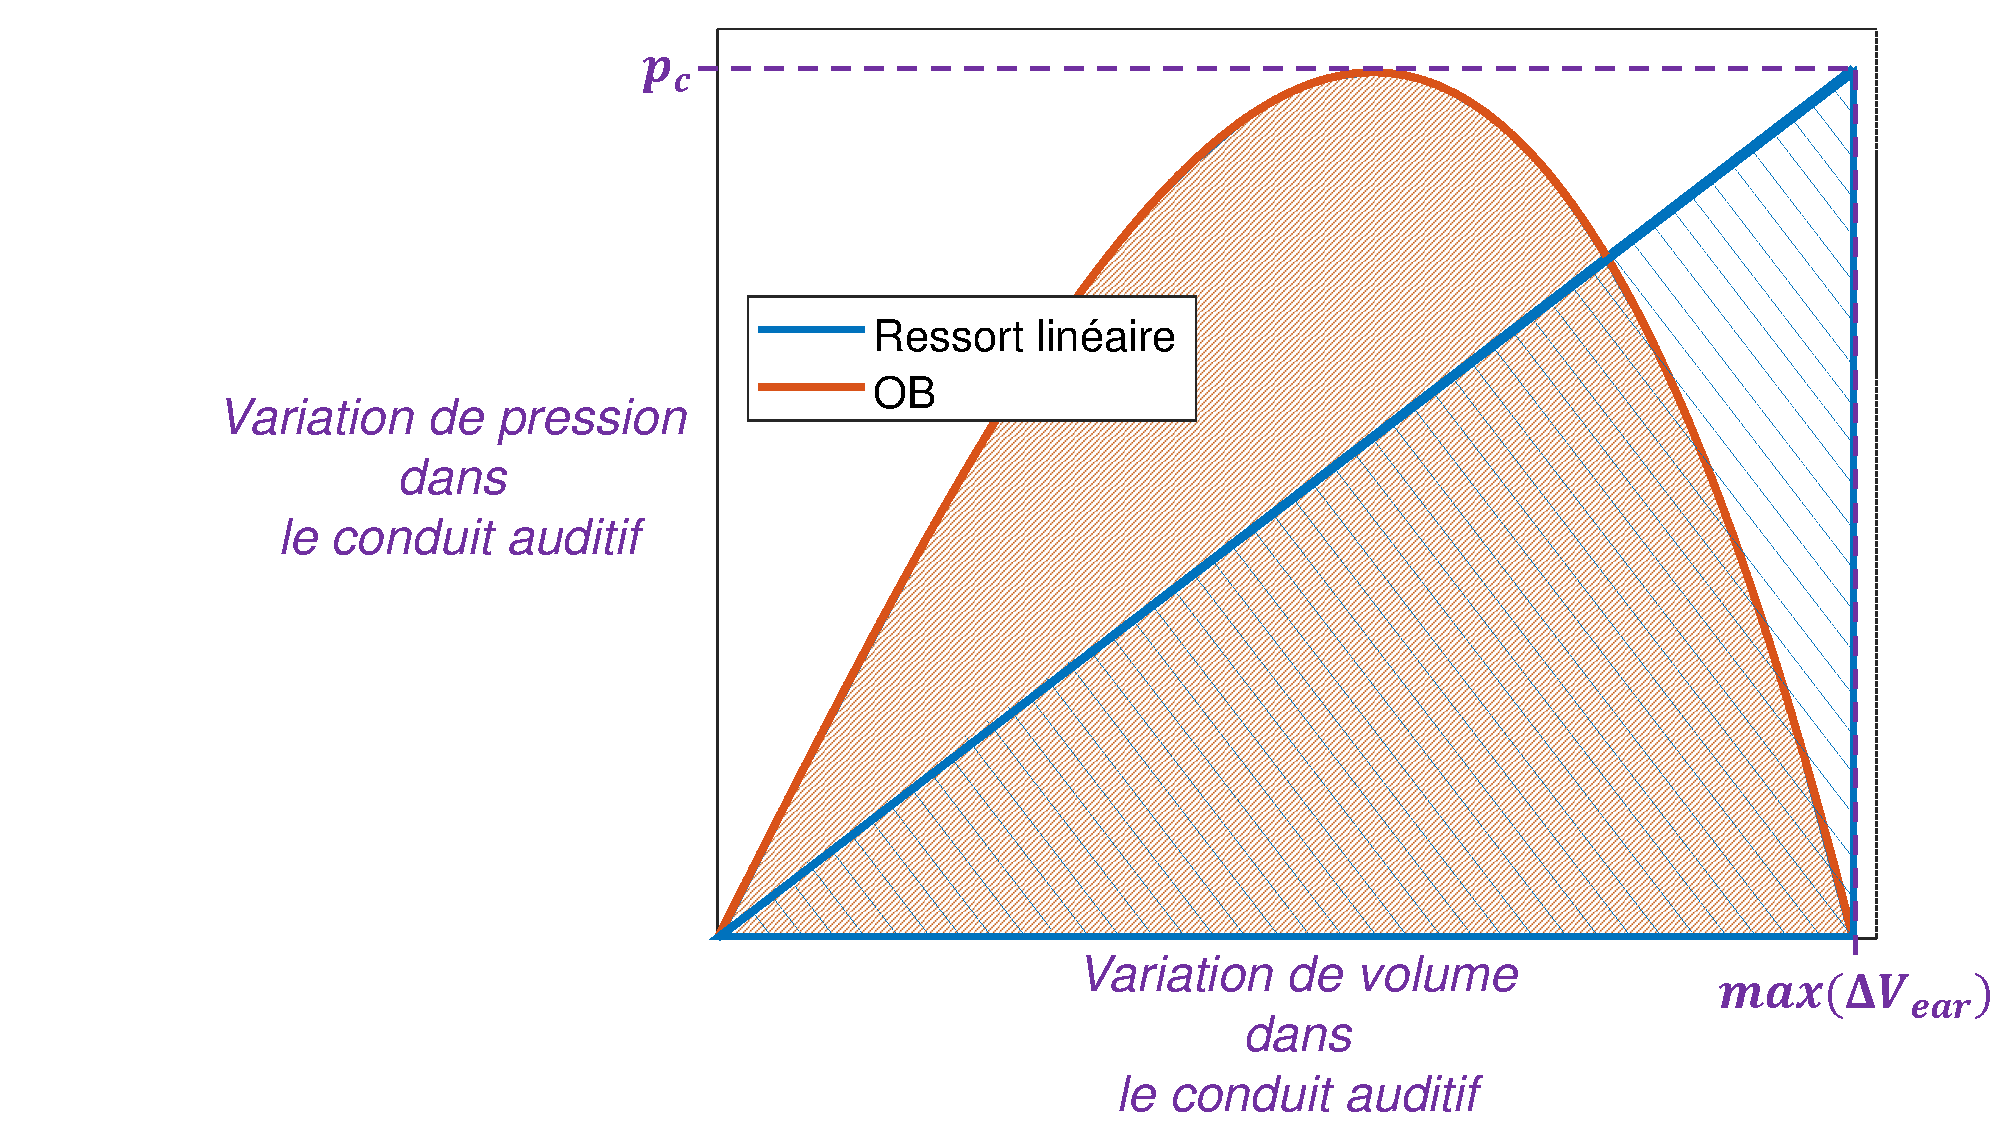
\includegraphics[trim={3.7cm 0cm 0cm 0.3cm},clip,width=0.6\textwidth]{../Chap2/Figure/force_elastique_lineaire_vs_OB.pdf}
	\caption{Évolution de la force élastique de l'OB et du meilleur ressort possible pour le gisement énergétique exploité}
	\label{fig:force_elastique_lineaire_vs_OB}
\end{center}	
\end{figure}
%%%%%%%%%%%%%%%%%%%%%%%%%%%%%%%%%%%%%%%%%

La figure \ref{fig:force_elastique_lineaire_vs_OB} montre alors l'allure de l'évolution de la force élastique $-F_{pis}$ de l'OB pour l'exploitation du gisement hydraulique. $F_{pis}$ est limitée pour ne pas induire une pression supérieure au seuil de confort $p_c$ dans l'oreille. Elle est également optimisée pour tirer profit du maximum de volume de fluide $\Delta V_{ear}$ disponible durant la mastication. L'aire sous la courbe orange de l'OB correspond alors à l'énergie maximale pouvant être emmagasinée par celui-ci, depuis la pompe à pression limite $p_c$ et variation de volume $\Delta V_{ear}$. Le comportement du prototype de récupérateur hydro-électromagnétique (fig. \ref{fig:debit_ear}) est équivalent, d'un point de vue mécanique, à un ressort linéaire \cite{Delnavaz2014}. De la même manière, le modèle du bouchon d'oreille d'oreille piézoélectrique intègre comme impédance mécanique un ressort linéaire issu de la raideur du matériau PVDF \cite{Delnavaz2013}. La raideur du ressort linéaire idéal maximisant l'énergie emmagasinée depuis la pompe serait alors égale au quotient $p_c/\Delta V_{ear}$ . L'énergie du bouchon d'oreille exploitable par ce ressort est donc équivalente à l'aire sous la courbe bleue de la figure \ref{fig:force_elastique_lineaire_vs_OB}.

Une première estimation de l'énergie maximale exploitable par l'OB pour un cycle de mastication peut alors être calculée. En considérant la variation de pression maximale $\Delta p_{ear} = p_c = 12$kPa, relevée dans l'étude de Bouchard-Roy \emph{et al.} \cite{Bouchard-Roy2020} pour une pression de gonflage de $p_{gon} = 27$kPa, ainsi qu'un volume déplacé maximal de $(\Delta V_{ear})_{max} = max(\Delta V_{ear}) = 60$mm$^3$ \cite{Delnavaz2012}, l'oreille pourrait au maximum fournir $E_{ear,m} = 0.72$mJ (éq. \ref{eq:Energie_max_oreille}).
\begin{equation}
	E_{ear,m} = p_c \cdot (\Delta V_{ear})_{max}
	\label{eq:Energie_max_oreille}
\end{equation}

Un mécanisme de stockage élastique linéaire permet d'exploiter la moitié de cette énergie d'après la figure \ref{fig:force_elastique_lineaire_vs_OB}. Un OB peut, quant à lui, emmagasiner une énergie égale à la hauteur de sa barrière de potentiel, soit $Ep_{bar,m} = 0.51$mJ avec les niveaux maximaux de pression et volume énoncés précédemment. Cette valeur est calculée avec l'équation \ref{eq:Barriere energie potentielle OB}, d'après les résultats du dimensionnement du système réalisé dans la section suivante (éq. \ref{eq:critere_confort}-\ref{eq:critere_course}). L'OB exploite donc la source à hauteur de 65\% de l'énergie disponible, contrairement à un oscillateur linéaire qui peut l'exploiter au maximum à 50\%.

L'optimisation de l'énergie exploitable appuie d'autant plus la pertinence de l'approche étudiée dans ce travail de thèse.
%/!\/!\/!\/!\/!\/!\/!\/!\/!\/!\/!\/!\/!\/!\/!\/!\/!\/!\/!\/!\/!\/!\/!\/!\%
\section{Critères de dimensionnement préliminaire}
\label{sec:2.5:Criteres de dimensionnement preliminaire}
%/!\/!\/!\/!\/!\/!\/!\/!\/!\/!\/!\/!\/!\/!\/!\/!\/!\/!\/!\/!\/!\/!\/!\/!\%
Le système de récupération d'énergie comprend de nombreux paramètres variables. Afin de les déterminer, il est d'abord nécessaire d'identifier les éléments technologiques fixes. Après quoi nous établirons les différents critères qui constituent les points de départ du dimensionnement global du système. 
	%////////////////////////////////////////////
	\subsection{Éléments technologiques fixes}
	\label{subsec:2.5.1_Elements technologiques fixes}	
	%////////////////////////////////////////////
\subsubsection*{\textit{GPA}}
%%%%%%%%%%%%%%%%%%%%%%%%%%%
\begin{table}[!htbp]
	\centering
	\rowcolors[]{2}{black!8}{}{
	\begin{tabular}{l|l|l}
		\rowcolor{blue!10}
		\toprule
		Paramètre & Valeur & [Unité]     \\
		\midrule
		$K$       & 0.256  & [$N/\mu m$] \\ 
		$\alpha$  & 0.105  & [$N/V$]     \\ 
		$C_0$     & 0.25   & [$\mu F$]   \\ 
		\bottomrule
	\end{tabular}}
	\caption{Paramètres pour l'APA50XS}
	\label{tab:parametres_apa50xs}
\end{table}
%%%%%%%%%%%%%%%%%%%%%%%%%%%
%%%%%%%%%%%%%%%%%%%%%%%%%%%
\begin{figure}[!htbp]
	\begin{center}
		\captionsetup{justification=centering}
		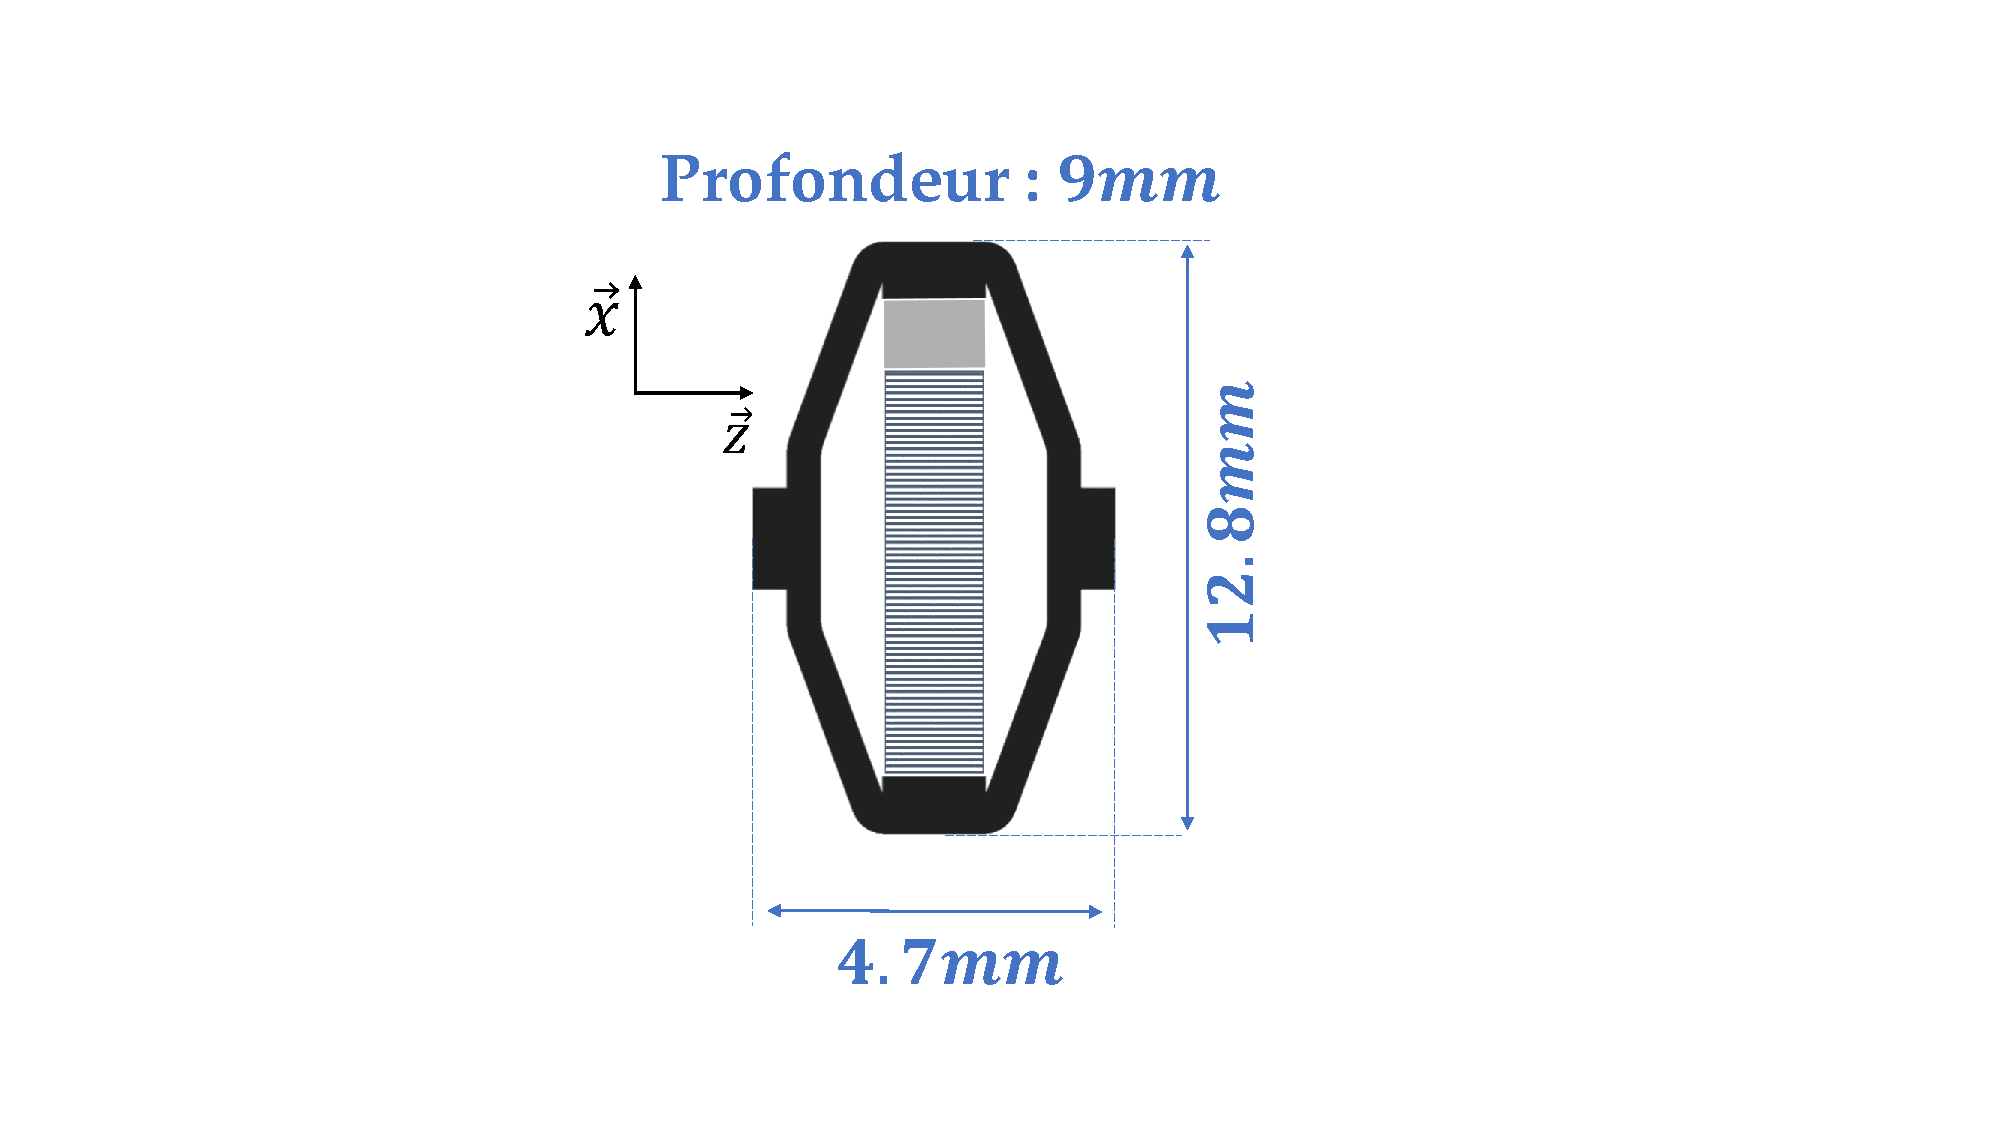
\includegraphics[trim={9.8cm 2.3cm 12.5cm 2.2cm},clip, width=0.15\textwidth]{../Chap2/Figure/dessin APA_dimensions.pdf}
		\caption{Dimensions de l'APA50XS}
		\label{fig:dimensions_apa50xs}
	\end{center}
\end{figure}
%%%%%%%%%%%%%%%%%%%%%%%%%%%% 

La transduction piézoélectrique sera réalisée en exploitant la technologie d'actionneur piézoélectrique amplifié (APA) [Cedrat Technologies] \cite{Huguet2018}. Ce-dernier sera exploité en tant que générateur pour notre application. Sachant que nous travaillons avec des niveaux d'efforts très faibles, il faut choisir une gamme de produits dont la rigidité est la plus faible possible. Par la suite, en jouant sur le flambement $\epsilon$, nous serons en mesure de gérer le niveau énergétique nécessaire afin de faire basculer M en tenant compte de l'énergie disponible dans l'oreille. Le produit qui doit être implémenté sur l'OB est un \emph{APA50XS}. Ce choix détermine la valeur des paramètres listés dans le tableau \ref{tab:parametres_apa50xs}, ainsi que l'encombrement du dispositif de transduction schématisé sur la figure \ref{fig:dimensions_apa50xs}.\\

\textbf{\textit{OB}}

Les liaisons pivots seront assurées par des lames souples qui seront dimensionnées dans le chapitre \ref{ch:6_Comportement du systeme de recuperation d’energie intra-auriculaire avec les composants caracterises experimentalement} lors de la conception et fabrication de l'OB.\\

\textbf{\textit{PH}}

Il faut limiter les frottements dans les PHs. Cependant, à l'échelle de l'application, il est difficile d'assurer l'étanchéité des pistons tout en offrant des pressions de fonctionnement faibles. L'actionnement sera donc assuré par les pistons de la gamme MQP4-10S du fabricant SMC qui admettent les pressions minimales de fonctionnement les plus faibles pour l'échelle du piston, soit, 1kPa. Cette valeur peut être mise en parallèle avec les variations de pressions mesurées dans le bouchon d'oreille en fonction de la pression de gonflage (tab. \ref{tab:Bouchard_deltaPmax}). En effet, les pressions offertes par le gisement hydraulique s'élèvent à 12kPa et sont par conséquent supérieures à la pression de fonctionnement des PHs. On peut également noter que, le choix technologique des pistons est également motivé par la mise en \oe{}uvre rapide offerte par une technologie certifiée et simple d'utilisation. Les caractéristiques techniques du piston MQP4-10S sélectionné sont présentées en annexe \ref{Ann:2_Vérin SMC série MQP}. Le diamètre de la tige mobile du piston est donc $D_p=4mm$. Les frottements du piston seront négligés dans un premier temps et seront évalués expérimentalement. \\

\textbf{\textit{Les VHs}}

La fonction de valve hydraulique sera assurée par un tube flexible fléchi au delà du flambement. Le couple de valves s'intègre comme des raideurs supplémentaires suivant l'axe d'oscillation de l'OB (éq. \ref{eq:OB+GPA+VH+piston}). La cinématique de leur comportement en fonction de la position de M est schématisée sur la figure \ref{fig:detail_flambement_MDOB}.
		%////////////////////////////////////////////
		\subsection{Contrainte de confort}
		\label{subsec:2.5.2_Contrainte de confort}	
		%////////////////////////////////////////////
La variation de pression générée dans le bouchon d'oreille produit naturellement une résistance mécanique proportionnelle sur les parois du conduit auditif. Cela pourrait occasionner une gêne qui, à notre connaissance, n'a pas été étudiée dans la littérature. On introduit alors le seuil de confort \mbox{$p_c = max(\Delta p_{ear})$} de l'utilisateur, qui est la pression maximale pouvant être induite dans le bouchon d'oreille. Cette pression résulte de l'impédance mécanique rencontrée par le PH. L'impédance de l'OB doit être prédominante devant celle des diverses pertes qui peuvent être de deux natures :
\begin{itemize}[label=$\circ$]
\item \emph{Hydrauliques}
	\begin{itemize}
		\item PdC linéaires du circuit hydraulique.
		\item PdC singulières dans les VHs et l'AH.
	\end{itemize}
\item \emph{Mécaniques}
	\begin{itemize}
		\item Frottements visqueux dans les pistons.
		\item Frottements de M dans l'air.
		\item Frottements secs au contact M-VH.
	\end{itemize}
\end{itemize}

La résistance $F_{ob}$ (éq. \ref{eq:F_OB_xxxxxx}) de l'OB passe par un maximum quand M se trouve à la position $x_c$ (fig. \ref{fig:x_crit}). Cette position peut être trouvée si on cherche la position de $x_m$ pour laquelle $\frac{dF_{ob}}{dx}$ s'annule, en négligeant les frottements secs. On définit alors $x_c$ par l'équation implicite \ref{eq:x_c} 
\begin{equation}
\dfrac{2K}{L^2}\biggl(3{x_c}^2-{x_0}^2\biggr) \ 
+\ \dfrac{\text{d}}{\text{d} x_m} \biggl(\frac{K_{VH}(x_m)}{a}\cdot \theta({x_m}) \biggr)
\ =\ 0
	\label{eq:x_c}
\end{equation} 
%%%%%%%%%%%%%%%%%%%%%%%%%%%
\begin{figure}[!htbp]
	\begin{center}
		\captionsetup{justification=centering}
		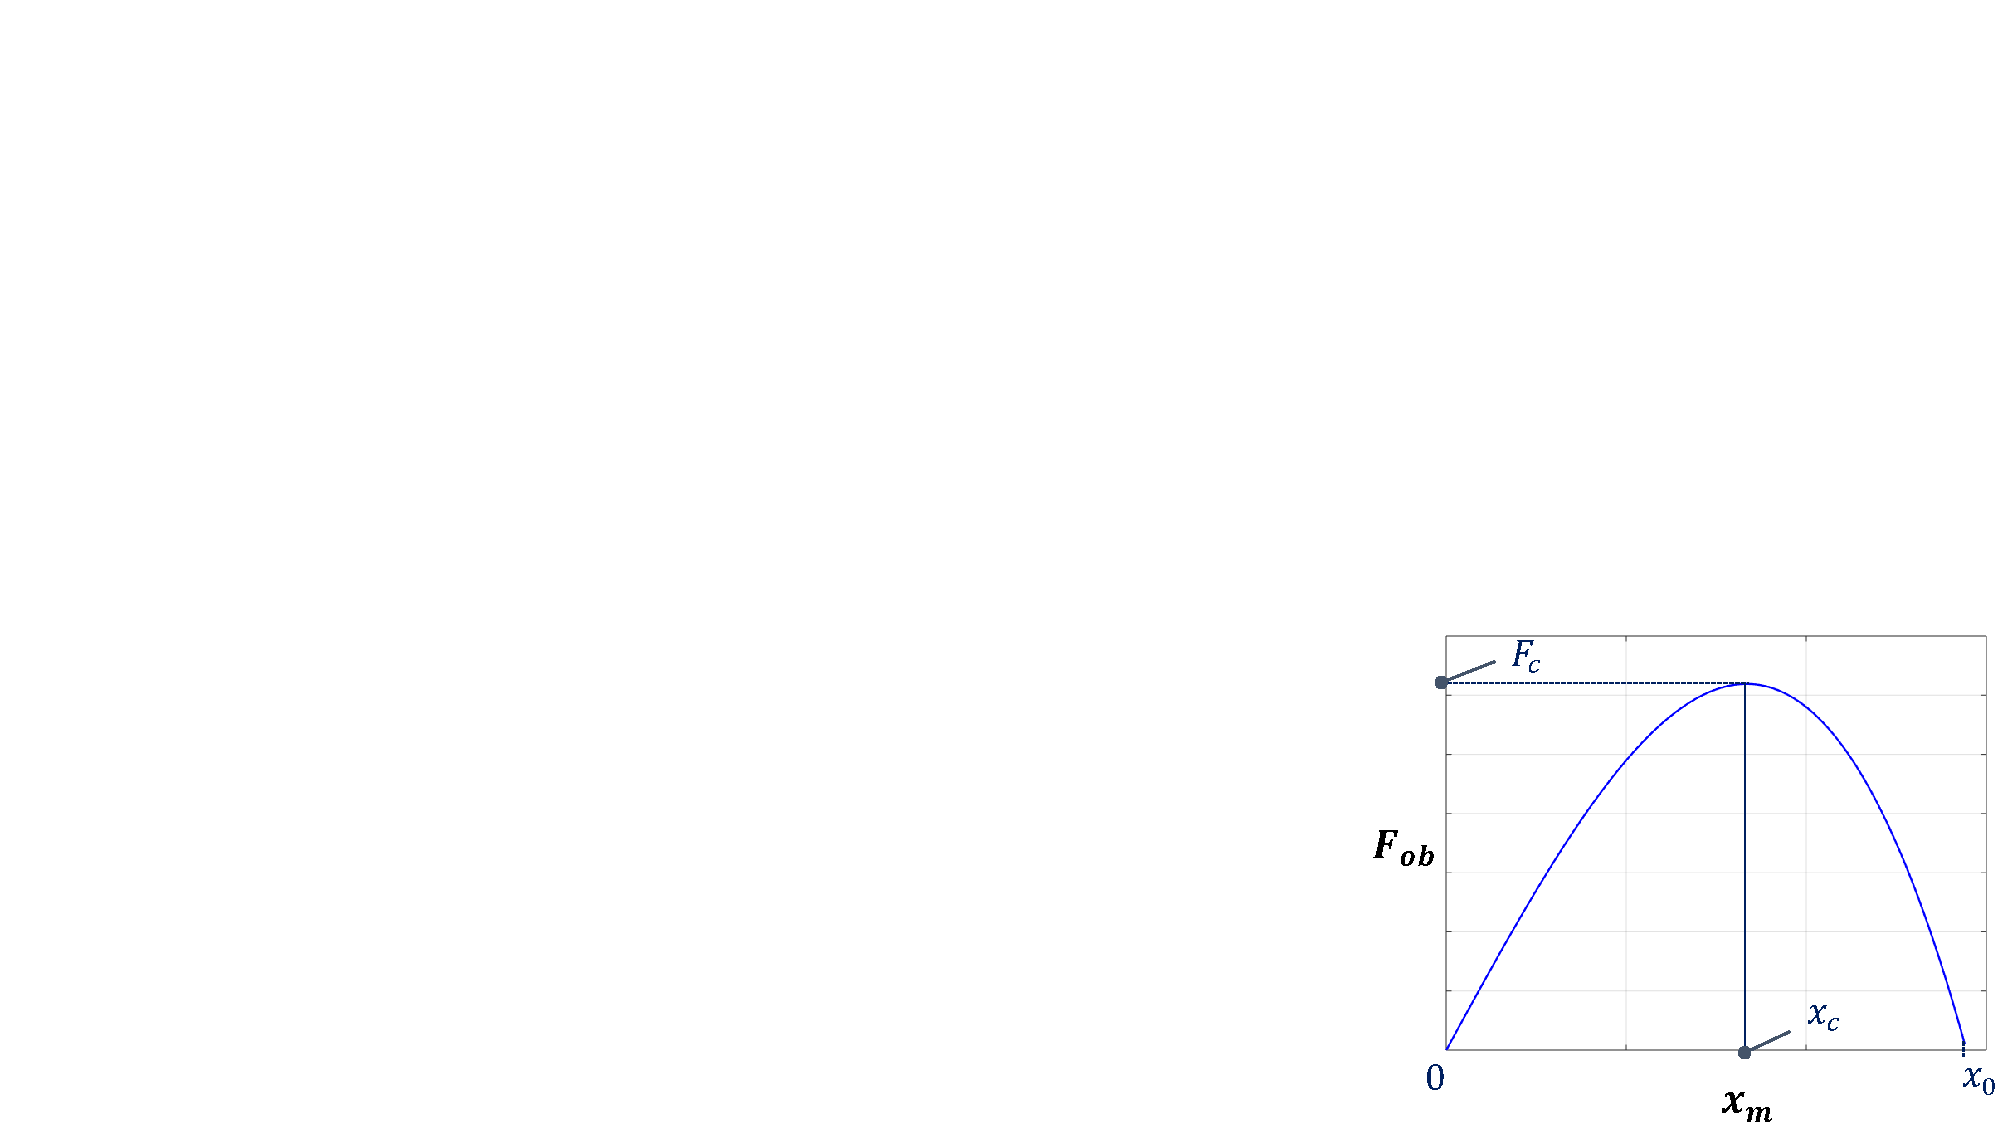
\includegraphics[trim={23cm 0cm 0cm 10.5cm},clip, width=0.5\textwidth]{../Chap2/Figure/x_crit.pdf}
		\caption{Forcé élastique de l'OB suivant l'axe $\vec{x}$}
		\label{fig:x_crit}
	\end{center}
\end{figure}
%%%%%%%%%%%%%%%%%%%%%%%%%%%% 
On notera $F_c$ l'impédance mécanique maximale rencontrée en actionnement QS par le PH. Celle-ci correspond alors à la résistance $F_{ob}$ de l'OB évaluée en $x_c$.\\
Connaissant les dimensions des pistons, on pourra alors établir l'inéquation suivante traduisant la contrainte de confort:
\begin{equation}
p_c > \frac{1}{a_h} \frac{F_c}{S_p}
\label{eq:critere_confort}
\end{equation}
Avec $p_c = max(\Delta p_{ear})$ la valeur maximale de la variation de pression $\Delta p_{ear}$ induite dans le bouchon d'oreille lors de la mastication, qu'on nommera seuil de confort. L'hypothèse QS et les pertes par frottement négligées peuvent être optimistes mais ont l'avantage d'offrir un outil de 
pré-dimensionnement simple pour assurer le critère de confort.
		%////////////////////////////////////////////
		\subsection{Contrainte de course}
		\label{subsec:2.5.3_Contrainte de course}	
		%////////////////////////////////////////////
La position rétractée $x_{p0}$ des pistons doit être supérieure à $x_0$ afin que les oscillations de M après basculement ne soient pas entravées par le piston dont l'alimentation hydraulique est fermée pour ce cycle de mastication. De plus, la variation de volume maximale $(\Delta V_{ear})_{max}$ dans le bouchon d'oreille doit être suffisante pour que la course d'un piston soit assurée entre $x_p = x_{p0}$ et  $x_p =0$ pour réaliser le basculement de M. On définit alors le coefficient $c_{xp}$ vérifiant l'inégalité suivante:
\begin{equation}
(\Delta V_{ear})_{max} > a_h\ S_p\ c_{xp}\ x_0~~~~\text{avec }~~~~c_{xp} = \dfrac{x_{p0}}{x_0}
\label{eq:critere_course}
\end{equation}
Ce critère permet de déduire la valeur de $x_{p0}$ afin que le la course des PHs soit assurée avec le volume de fluide $(\Delta V_{ear})_{max}$ déplacé.
		%////////////////////////////////////////////
		\subsection{Contrainte d'encombrement}
		\label{subsec:2.5.4_Contrainte d'encombrement}	
		%////////////////////////////////////////////
Le système entier a pour finalité d'être intégré dans un boîtier de type appareil auditif ou implant cochléaire à l'extérieur du CA. Les dimensions standard font V$_{boitier}$ = 50x20x10mm pour ces dispositifs. Les dimensions de l'OB, du diamètre des PHs et des diamètres des VH seront donc dimensionnés en cohérence avec l'échelle de l'application. Ainsi, un premier dimensionnement permettra d'obtenir un comportement semblable à celui du récupérateur idéal intégrable au boîtier. 

Les composants au c\oe{}ur du fonctionnement du dispositif, tels que les l'OB, le GPA, le bouchon d'oreille, ainsi que les VHs, sont susceptibles de présenter des défis d'intégration trop complexes pour pouvoir assurer le fonctionnement du système de récupération. Il est donc pertinent, au regard de la preuve de concept visée, d'envisager la fabrication et la caractérisation expérimentale de ces composants à l'échelle même de l'application. Le reste des composants, tels que l'AH, les PHs et le circuit hydraulique les reliant, seront dans un premier temps envisagés à une échelle supérieure à celle de l'application afin de faciliter la mise en \oe{}uvre d'un premier démonstrateur. 

Le premier stade des essais expérimentaux visera à valider la preuve de concept introduite par cette nouvelle architecture de récupérateur d'énergie uniquement. En ce sens, le travail de thèse se concentre sur la validation expérimentale de l'innovation architecturale apportée par le couplage des VHs à base de tubes flexibles et de l'OB intégrant un GPA. L'étude de l'architecture des PHs, du découpleur hydraulique, ainsi que de l'AH ne seront, en conséquence, pas abordés. Pour des raisons de simplification expérimentale, le corps du vérin hydraulique ne sera pas en cohérence avec l'échelle de l'application. Les aspects d'intégration pourront être traités sur un travail réalisable en aval, avec les conclusions des travaux présentés dans ce manuscrit.
%/!\/!\/!\/!\/!\/!\/!\/!\/!\/!\/!\/!\/!\/!\/!\/!\/!\/!\/!\/!\/!\/!\/!\/!\%
\section{Modèle numérique du système global}
\label{subsec:2.6_Modele numerique du systeme global}
%/!\/!\/!\/!\/!\/!\/!\/!\/!\/!\/!\/!\/!\/!\/!\/!\/!\/!\/!\/!\/!\/!\/!\/!\%
		%////////////////////////////////////////////
		\subsection{Objectif du modèle}
		\label{2.6.1_Objectif du modele}
		%////////////////////////////////////////////
Dans cette section, nous présentons les résultats du modèle numérique que nous avons établi, suite à la mise en équation analytique du comportement du système global avec les équations \ref{eq:critere_confort} et \ref{eq:critere_course}. L'objectif sera de simuler l'évolution des paramètres du système en utilisant en entrée de celui-ci le débit imposé par le bouchon d'oreille (fig. \ref{fig:debit_ear}). On cherche à montrer la preuve de concept théorique du fonctionnement du système ainsi développé. La courbe caractéristique $q_{ear}=f(p_{ear})$ n'a pas encore été établie pour l'oreille sous l'impédance mécanique de l'OB suivant $\vec{x}$ (éq. \ref{eq:F_OB_xxxxxx}). Durant cette première phase, le bouchon d'oreille est donc assimilé à une source de débit parfaite. Nous allons donc déterminer le comportement hydraulique nécessaire pour que les VHs puissent assurer la bonne dynamique de fonctionnement cyclé du mouvement de M.
		%////////////////////////////////////////////
		\subsection{Présentation du modèle}
		\label{2.6.2_Presentation du modele}
		%////////////////////////////////////////////
Le dimensionnement des paramètres respectifs de l'OB et du circuit hydraulique est réalisé à partir des critères préliminaires énoncés dans la section \ref{sec:2.5:Criteres de dimensionnement preliminaire}. La résolution des équations définissant l'état du système pour les différentes phases se fait de façon numérique grâce à l’établissement d'un modèle multiphysique avec l'outil Simulink.

La pression maximale admissible dans l'oreille est fixée à \mbox{$p_c=1$kPa}. Le débit imposé à l'entrée du système est issu de mesures temporelles de variation de volume réalisés par le laboratoire partenaire CRITIAS de l'ÉTS de Montréal sur un sujet humain. Les mesures ont été faites dans les conditions des essais avec le récupérateur hydro-électromagnétique (fig. \ref{fig:Critias_electromag_schema}). Une interpolation linéaire est réalisée sur le débit en fonction du temps, avant  de l'imposer en entrée du modèle numérique. Son allure est visible sur la figure \ref{fig:debit_ear}. La valeur de $(\Delta V_{ear})_{max}$ sera, de surcroît, extraite depuis cette mesure pour le dimensionnement. Par ailleurs, les pertes de charges liées à l'AH, ainsi qu'au découpleur de pression, seront négligées dans le modèle numérique de pré-dimensionnement. Les pertes hydrauliques individuelles de chacun des composants pourront, par la suite, être estimées expérimentalement afin d'affiner le modèle.

Un cycle de mastication du point de vue du système de récupération peut se décomposer en deux grandes étapes que sont l'actionnement QS et les oscillations. La première consiste en la poussée de M par le piston, sur une course depuis une position d'équilibre stable, vers la position d'équilibre stable symétrique. La seconde intègre l'oscillation de M dont l'énergie est en partie convertie en électricité par le GPA. 

Les équations différentielles définissant le système sont résolues en parallèle et de façon indépendante les unes des autres. Les différentes conditions dépendantes des positions de M, ainsi que celles des pistons, permettent de gérer, à l'aide des variables booléennes, les transitions du système depuis un état vers un autre. Ces dernières sont successivement décrites dans les parties \ref{subsubsec:2.5.2.c:Phase d'actionnement de M} et \ref{subsubsec:2.5.2.c:Phase d'oscillations de M} qui suivent. Un code couleur est mis en place pour différencier les \textcolor{c}{\underline{variables d'entrée}}, \textcolor{b}{\underline{les paramètres constants}} et les \textcolor{a}{\underline{variables de sortie}} du système global.
	%*************
	\subsubsection{Phases d'actionnement de M}
	\label{subsubsec:2.5.2.c:Phase d'actionnement de M}
	%*************
Les phases d'actionnement \emph{1a} et \emph{1b} du cycle de mastication du point de vue de l'OB sont illustrées et détaillées dans le tableau \ref{tbl:act_top}. La première (phase 1a) correspond à l'approche du piston qui n'est, au départ, pas en contact avec M. La seconde (phase 1b) correspond au déplacement QS du système solidaire \{PH + M\} vers $x=0$, depuis $x=-x_0$.\\
\subsubsection*{Phase1a}%----------------
La VH alimentant le piston \emph{haut} est fermée car M se trouve à la position d'équilibre basse en $x_m=-x_0$. Le débit $q_{ear}$ est alors imposé à l'entrée du système. Durant cette phase, le comportement des deux branches hydrauliques est donc soumis aux systèmes d'équations (\ref{eq:Phase1a_hydraulique_top}$-$\ref{eq:Phase1a_conservation_debit_ear}).\\
Les conditions initiales au départ de cette phase sont les suivantes : 
\begin{itemize}[label=$\bullet$]
	\item La VH$_h$ est fermée et la VH$_b$ est ouverte.
 	\item Pas de contact entre le piston et la masse.
	\item $x_m=-x_0$.
\end{itemize}
% %%%%%%%%%%%%%%%%%%%%%%%%%%%%%%%%
\begin{subnumcases}{}
$$\left\{
    \begin{array}{l}
\textcolor{a}{p_{ph}}\ \textcolor{b}{S_{p}} = \textcolor{b}{C_{p}}\ \textcolor{a}{\dot{x}_{ph}}\\
\textcolor{a}{p_{ear}} = \textcolor{b}{p_{gon} } + \frac{1}{\textcolor{b}{a_h}}\biggl(\textcolor{a}{p_{ph}} + 
\dfrac{\textcolor{b}{\Delta p_{cl}}(\text{sign}(\textcolor{c}{q_{ear}}))\cdot \textcolor{b}{Cf}(\textcolor{a}{x_m})\ \textcolor{a}{q_f}^2}{\textcolor{b}{\Delta p_{cl}}(\text{sign}(\textcolor{c}{q_{ear}}))\ +\ \textcolor{b}{Cf}(\textcolor{a}{x_m})\ \textcolor{a}{q_f}^2} \bigg)\\
\textcolor{a}{q_{h}} = \textcolor{b}{S_p}\ \textcolor{a}{\dot{x}_{ph}}    
    \end{array}
\right.$$
\label{eq:Phase1a_hydraulique_top}\\
$$\left\{
   \begin{array}{l}
\textcolor{a}{p_{pb}}\ \textcolor{b}{S_{p} }= \textcolor{b}{C_{p}}\ \textcolor{a}{\dot{x}_{pb}}\\
\textcolor{a}{p_{ear}} = \textcolor{b}{p_{gon} }+ \frac{1}{\textcolor{b}{a_h}}\biggl(\textcolor{a}{p_{pb} }+ 
\dfrac{\textcolor{b}{\Delta p_{cl}}(\text{sign}(\textcolor{c}{q_{ear}}))\cdot \textcolor{b}{Cf_0}\ \textcolor{a}{q_h}^2}{\textcolor{b}{\Delta p_{cl}}(\text{sign}(\textcolor{c}{q_{ear}}))\ +\ \textcolor{b}{Cf_0}\ \textcolor{a}{q_h}^2} \biggr)\\
\textcolor{a}{q_{b}} = \textcolor{b}{S_p}\ \textcolor{a}{\dot{x}_{pb}}
    \end{array}
\right.$$
\label{eq:Phase1a_hydraulique_bot}\\
$$~~~~~\textcolor{c}{q_{ear}} = \textcolor{b}{a_h}(\textcolor{a}{q_h} + \textcolor{a}{q_b})$$
\label{eq:Phase1a_conservation_debit_ear}
\end{subnumcases} 
%%%%%%%%%%%%%%%%%%%%%%%%%%%%%%%%
La condition de changement de phase est la suivante : Le piston hydraulique \emph{bas} (PH$_b$) entre en contact avec M.
\subsubsection*{Phase1b} %----------------
Le PH$_b$ arrive en contact avec M. On suppose que les deux composants forment alors un système solidaire qui va se déplacer jusqu'à la position $x=0$. On a donc l'égalité $x_{pb} = x_m$ durant cette phase. Les systèmes d'équations (\ref{eq:Phase1b_hydraulique_top}$-$\ref{eq:Phase1b_F_bis}) décrivent le comportement multiphysique couplé des deux composants M et PH$_b$ en contact. Dans l'équilibre dynamique du PH$_b$, exprimé dans le système d'équations \ref{eq:Phase1b_hydraulique_bot}, la contre-réaction $F_{ob}$ de l'OB s'ajoute et s'exprime par l'équation \ref{eq:Phase1b_F_bis}. Celle-ci est la cause principale de la variation de pression $\Delta p_{ear}$ (éq. \ref{eq: variation de pression DeltaP_ear}) induite dans l'oreille.\\
Les conditions initiales au départ de cette phase sont les suivantes : 
\begin{itemize}[label=$\bullet$]
	\item La VH$_h$ est fermée et la VH$_b$ est ouverte.
 	\item Contact permanent entre le piston \emph{bas} et la masse.
	\item $x_m=-x_0$.
\end{itemize}
%%%%%%%%%%%%%%%%%%%%%%%%%%%%%%%%
\begin{subnumcases}{}
$$\left\{
	\begin{array}{l}
\textcolor{a}{p_{ph}}\ \textcolor{b}{S_{p}} = \textcolor{b}{C_{p}}\ \textcolor{a}{\dot{x}_{ph}}\\
\textcolor{a}{p_{ear}} = \textcolor{b}{p_{gon} } + \frac{1}{\textcolor{b}{a_h}}\biggl(\textcolor{a}{p_{ph}} + 
\dfrac{\textcolor{b}{\Delta p_{cl}}(\text{sign}(\textcolor{c}{q_{ear}}))\cdot \textcolor{b}{Cf}(\textcolor{a}{x_m})\ \textcolor{a}{q_f}^2}{\textcolor{b}{\Delta p_{cl}}(\text{sign}(\textcolor{c}{q_{ear}}))\ +\ \textcolor{b}{Cf}(\textcolor{a}{x_m})\ \textcolor{a}{q_f}^2} \bigg)\\
\textcolor{a}{q_{h}} = \textcolor{b}{S_p}\ \textcolor{a}{\dot{x}_{ph}}      
	\end{array}
\right.$$
\label{eq:Phase1b_hydraulique_top}\\
$$\left\{
	\begin{array}{l}
\textcolor{a}{F_{ob}} - \textcolor{a}{p_{pb}}\ \textcolor{b}{S_{p} }= \textcolor{b}{C_{p}}\ \textcolor{a}{\dot{x}_{pb}}\\
\textcolor{a}{p_{ear}} = \textcolor{b}{p_{gon} }+ \frac{1}{\textcolor{b}{a_h}}\biggl(\textcolor{a}{p_{pb} }+ 
\dfrac{\textcolor{b}{\Delta p_{cl}}(\text{sign}(\textcolor{c}{q_{ear}}))\cdot \textcolor{b}{Cf_0}\ \textcolor{a}{q_h}^2}{\textcolor{b}{\Delta p_{cl}}(\text{sign}(\textcolor{c}{q_{ear}}))\ +\ \textcolor{b}{Cf_0}\ \textcolor{a}{q_h}^2} \biggr)\\
\textcolor{a}{q_{b}} = \textcolor{b}{S_p}\ \textcolor{a}{\dot{x}_{pb}}
	\end{array}
\right.$$
\label{eq:Phase1b_hydraulique_bot}\\
$$
~~~~~\textcolor{c}{q_{ear}} = \textcolor{b}{a_h}(\textcolor{a}{q_h} + \textcolor{a}{q_b})
$$
\label{eq:Phase1b_conservation_debit_ear}\\
$$
~~~~~\textcolor{a}{F_{ob}} = \frac{2\textcolor{b}{K\ {x_0}}^2}{\textcolor{b}{L}^2}\biggl(\frac{{\textcolor{a}{{x}_{pb}}^2}}{\textcolor{b}{{x_0}}^2} -1\biggr)\textcolor{a}{x_{pb}} - \biggl( \frac{\textcolor{b}{K_{VH}}}{\textcolor{b}{a}} \biggr) \arctan \biggl(\frac{\textcolor{a}{x_{pb}}}{\textcolor{b}{a}} \biggr) + \textcolor{b}{F_f}\sign(\textcolor{a}{\dot{x}_{pb}})
$$
\label{eq:Phase1b_F_bis}
\end{subnumcases} 
%%%%%%%%%%%%%%%%%%%%%%%%%%%%%%%%
La condition de changement de phase est la suivante : M franchit l'axe $x=0$.
	%*************
	\subsubsection{Phase d'oscillations de M}
	\label{subsubsec:2.5.2.c:Phase d'oscillations de M}
	%*************
M franchit le seuil d'équilibre instable et possède alors un comportement de type lâcher libre vers la position d'équilibre stable haute. La VH$_b$ se ferme et la VH$_h$ s'ouvre. Aucun des pistons n'est en contact avec la masse. La conversion d'énergie se fait au travers du GPA, dont le comportement électromécanique est régi par le système d'équations \ref{eq:Phase2_OB+GPA}, jusqu'à l'arrêt de M.\\
Les conditions initiales au départ de cette phase sont les suivantes : 
\begin{itemize}[label=$\bullet$]
	\item La VH$_h$ est ouverte et la VH$_b$ est fermée.
 	\item Pas de contact entre les pistons et la masse.
	\item $x_m=0$.
 	\item $\dot{x}_m$ égal à sa valeur au dernier incrément de la phase précédente.
\end{itemize}
%%%%%%%%%%%%%%%%%%%%%%%%%%%%%%%%
\begin{subnumcases}{}
$$\left\{
    \begin{array}{l}
\textcolor{a}{p_{ph}}\ \textcolor{b}{S_{p}} = \textcolor{b}{C_{p}}\ \textcolor{a}{\dot{x}_{ph}}\\
\textcolor{a}{p_{ear}} = \textcolor{b}{p_{gon} } + \frac{1}{\textcolor{b}{a_h}}\biggl(\textcolor{a}{p_{ph}} + 
\dfrac{\textcolor{b}{\Delta p_{cl}}(\text{sign}(\textcolor{c}{q_{ear}}))\cdot \textcolor{b}{Cf_0}\ \textcolor{a}{q_h}^2}{\textcolor{b}{\Delta p_{cl}}(\text{sign}(\textcolor{c}{q_{ear}}))\ +\ \textcolor{b}{Cf_0}\ \textcolor{a}{q_h}^2} \biggr)\\
\textcolor{a}{q_{h}} = \textcolor{b}{S_p}\ \textcolor{a}{\dot{x}_{ph}}      
    \end{array}
\right.$$
\label{eq:Phase2_hydraulique_top}\\
$$\left\{
   \begin{array}{l}
\textcolor{a}{p_{pb}}\ \textcolor{b}{S_{p} }= \textcolor{b}{C_{p}}\ \textcolor{a}{\dot{x}_{pb}}\\
\textcolor{a}{p_{ear}} = \textcolor{b}{p_{gon} }+ \frac{1}{\textcolor{b}{a_h}}\biggl(\textcolor{a}{p_{pb} }+ 
\dfrac{\textcolor{b}{\Delta p_{cl}}(\text{sign}(\textcolor{c}{q_{ear}}))\cdot \textcolor{b}{Cf}(\textcolor{a}{x_m})\ \textcolor{a}{q_f}^2}{\textcolor{b}{\Delta p_{cl}}(\text{sign}(\textcolor{c}{q_{ear}}))\ +\ \textcolor{b}{Cf}(\textcolor{a}{x_m})\ \textcolor{a}{q_f}^2} \bigg)\\
\textcolor{a}{q_{b}} = \textcolor{b}{S_p}\ \textcolor{a}{\dot{x}_{pb}}
    \end{array}
\right.$$
\label{eq:Phase2_hydraulique_bot}\\
$$
~~~~~\textcolor{c}{q_{ear}} = \textcolor{b}{a_h}(\textcolor{a}{q_h} + \textcolor{a}{q_b})
$$
\label{eq:Phase2_conservation_debit_ear}\\
$$\left\{
   \begin{array}{l}
\textcolor{a}{\ddot{x}} = - \frac{2\textcolor{b}{K x_0}^2}{\textcolor{b}{mL}^2}\biggl(\frac{\textcolor{a}{x_m}^2}{\textcolor{b}{x_0}^2} -1\biggr)\textcolor{a}{x_m} - \biggl( \frac{\textcolor{b}{\mu}}{\textcolor{b}{m}} \biggr) \textcolor{a}{\dot{x}_m} - \frac{2\textcolor{b}{\alpha} \textcolor{a}{U_p\ x_m}}{\textcolor{b}{mL}} - \biggl( \frac{\textcolor{b}{K_{VH}}}{\textcolor{b}{ma}} \biggr) \arctan \biggl(\frac{\textcolor{a}{x_m}}{\textcolor{b}{a}} \biggr) - \frac{\textcolor{b}{F_f}\sign(\textcolor{a}{\dot{x}_m})}{\textcolor{b}{m}} \\
\frac{\textcolor{a}{U_p}}{\textcolor{b}{R_{ch}}} = \frac{2\textcolor{b}{\alpha}\textcolor{a}{x_m}\textcolor{a}{\dot{x_m}}}{\textcolor{b}{L}} - \textcolor{b}{C_0}\textcolor{b}{\dot{U}_p}
    \end{array}
\right.$$
\label{eq:Phase2_OB+GPA}
\end{subnumcases} 
Cette phase se termine lorsque M est arrêtée est que les deux pistons sont rétractés. À ce moment là peut débuter la phase d'actionnement suivante, du côté piston \emph{haut}, avec les conditions initiales équivalentes aux conditions de fin de cette phase à savoir :
\begin{itemize}[label=$\bullet$]
	\item La VH$_h$ est ouverte et la VH$_b$ est fermée
 	\item Pas de contact entre les pistons et la masse.
	\item $x_m=-x_0$
\end{itemize}
%%%%%%%%%%%%%%%%%%%%%%%%%%%%%%%%
	%*************
	\subsubsection{Comportement hydraulique idéal des VHs}
	\label{subsubsec:2.5.2.a:Comportement hydraulique cible des VHs}
	%*************
Le coefficient de pertes de charges $Cf$ traduit la résistance hydraulique dans les VHs (éq. \ref{eq:Cf_definition}). Ce coefficient doit être une fonction paire de $x_m$, de façon à respecter la symétrie de l'actionnement de M depuis les deux positions d'équilibre stables $\pm x_0$. À ce stade de l'étude, la loi de comportement $Cf=f(x_m)$ est cependant inconnue. La littérature ne propose en effet aucun modèle analytique pour les pertes de charges au travers d'un tube de section flambée car c'est un phénomène qui est généralement perçu comme étant néfaste pour un écoulement.\\
Nous savons par ailleurs qu'à $x_m=0$ on a $Cf_h = Cf_b = Cf_0$ avec $Cf_h$ et $Cf_b$ les coefficients de PdC respectifs de VH$_h$ et VH$_b$. On note aussi au temps $t=0$ la valeur des différents paramètres comme suit :
\begin{equation}
\begin{dcases}
x_m(t=0)\ =\ -x_0\\
Cf_h(-x_0)\ =\ Cf_f\\
Cf_b(-x_0)\ =\ Cf_0
\end{dcases}
\end{equation}
L'écoulement se produit en parallèle dans les deux branches hydrauliques. Il faut donc maximiser le rapport de fermeture $(r_{Cf})$ défini à l'équation \ref{eq:r_Cf} pour diriger le fluide dans la branche ouverte.
\begin{equation}
r_{Cf}\ =\ \frac{Cf(\text{VH fermée})}{Cf(\text{VH ouverte})}
\label{eq:r_Cf}
\end{equation}
Qui vaut alors à $t=0$ :
\begin{equation}
r_{Cf}(t=0)\ =\ (r_{Cf})_{min}\ =\ \frac{Cf_h(-x_0)}{Cf_b(-x_0)}\ =\ \frac{Cf_f}{Cf_0} 
\label{eq:(r_Cf)_min}
\end{equation}
Une valeur minimale permettra que l'écoulement soit privilégié vers le piston du \emph{bas}. Il est alors possible, à travers un processus itératif, de quantifier le rapport $(r_{Cf})_{min}$. Pour cela, lorsque M entre en contact avec la VH, une loi de comportement linéaire est imposée pour l'évolution de $Cf(x_m)$. Elle se définit par l'équation \ref{eq:Cf(x_m) evolution lineaire}.
\begin{align}
Cf\ &=\ Cf_0\ +\ \frac{Cf_f-Cf_0}{x_0}x_m \\
	&=\ Cf_0\biggl(1+\biggl(\dfrac{1}{r_{Cf}}-1\biggr)\dfrac{x_m}{x_0}\biggr)
\label{eq:Cf(x_m) evolution lineaire}
\end{align}	
	%////////////////////////////////////////////
	\subsection{Simulations et résultats}
	\label{subsec:2.5.3:Simulation et resultats}
	%////////////////////////////////////////////
%%%%%%%%%%%%%%%%%%%%%%%%%%%%%%%%%	
\begin{table}	
	\begin{minipage}[b]{0.5\textwidth}
		\centering
		\begin{tabular}{c|c|c}
		\rowcolor{blue!10}    
\toprule
\multicolumn{1}{c}{~~\textbf{Paramètre}~~}  & \multicolumn{1}{c}{~~\textbf{Valeur}~~} & \multicolumn{1}{c}{~~\textbf{[Unité]}~~}  \\
\midrule
$K$					&	0.256			& [$N/\mu m$]			\\ \hline
$x_0$				&	0.49			& [$mm$] 				\\ \hline
$L$					&	16.0			& [$mm$] 				\\ \hline
$M$					&	5.88			& [$g$] 				\\ \hline
$x_{p0}$			&	0.69			& [$mm$] 				\\ \hline
$R_{ch}$			&	15.5			& [$k\Omega$] 			\\ \hline
$\alpha$			&   0.105			& [$N/V$] 				\\ \hline
$C_0$	   			&	0.25			& [$\mu F$]				\\ \hline
$Q$ 				&	50				& [~~] 					\\ \hline
\textcolor{red}{$\eta_g$}		& 	\textcolor{red}{67.1}	& \textcolor{red}{[$\%$]}		\\ 
\bottomrule
		\end{tabular}
		\caption{Parametres électromécaniques}
		\label{tab:parametres électromécaniques}
	\end{minipage}
	\begin{minipage}[b]{0.5\textwidth}
		\centering
		\begin{tabular}{c|c|c}
		\rowcolor{blue!10}   
\toprule
\multicolumn{1}{c}{~~\textbf{Paramètre}~~}  & \multicolumn{1}{c}{~~\textbf{Valeur}~~} & \multicolumn{1}{c}{~~\textbf{[Unité]}~~}  \\
\midrule
$D_p$  	   				&	4				& [$mm$]					\\ \hline
$a_h$					&	7.2				& [~~]						\\ \hline
$p_c$					&	1				& [$kPa$]					\\ \hline
$\Delta V{ear,m}$		& 60				& [$mm^3$]					\\ \hline
\textcolor{red}{$Cf_0$}			&	\textcolor{red}{5.4e16}	&\textcolor{red}{[$Pa.s^2m^{-6}$]}	\\ \hline
\textcolor{red}{$Cf_f$}			&	\textcolor{red}{6.4e17}	&\textcolor{red}{[$Pa.s^2m^{-6}$]}	\\
\bottomrule 
		\end{tabular}
		\caption{Paramètres hydrauliques}
		\label{tab:parametres_hydrauliques}
\end{minipage}
\end{table}
%%%%%%%%%%%%%%%%%%%%%%%%%%%%%%%%%
En faisant évoluer $r_{Cf}$, on arrive à une valeur de $Cf_f$ pour laquelle l'écoulement vers le piston du \emph{bas} est privilégié. On en déduit que $(r_{Cf})_{min}\approx 10$ est l'objectif à atteindre pour dimensionner un couple de VHs fonctionnelles. Au terme du processus d'essais-erreurs, on établit la figure \ref{fig:simu_pos_debit_Cf_pression_1CYCLE} qui montre l'évolution des positions des pistons et de la masse, l'évolution des débits et pressions respectifs dans les pistons et le bouchon d'oreille, ainsi que l'évolution des coefficients de PdC dans les VHs.

Les trois étapes $1_a$, $1_b$ et $2$, du fonctionnement du système durant un cycle de mastication, sont mises en évidence. Les deux traits verticaux pointillés marquent le passage d'une étape à une autre. Les débits positifs traduisent le fluide sortant du bouchon d'oreille. Les tableaux \ref{tab:parametres électromécaniques}et \ref{tab:parametres_hydrauliques} listent les valeurs des paramètres clé du modèle de pré-dimensionnement simulé en mettant en évidence trois paramètres obtenus au terme du processus essais-erreurs. L'OB est dimensionné de façon à induire une pression au maximum égale au seuil de confort $p_c=1kPa$. Le léger dépassement de ce seuil est dû aux PdC dans la branche hydraulique qui actionne, durant l'étape de poussée $1_b$. La position initiale du piston \emph{haut} est calculée de façon à ne pas amener de perturbations durant la phase $2$ de récupération.
%%%%%%%%%%%%%%%%%%%%%%%%%%%%%%%%%%%%%%%%%
\begin{figure}[!ht]
\begin{center}
    \captionsetup{justification=centering}
	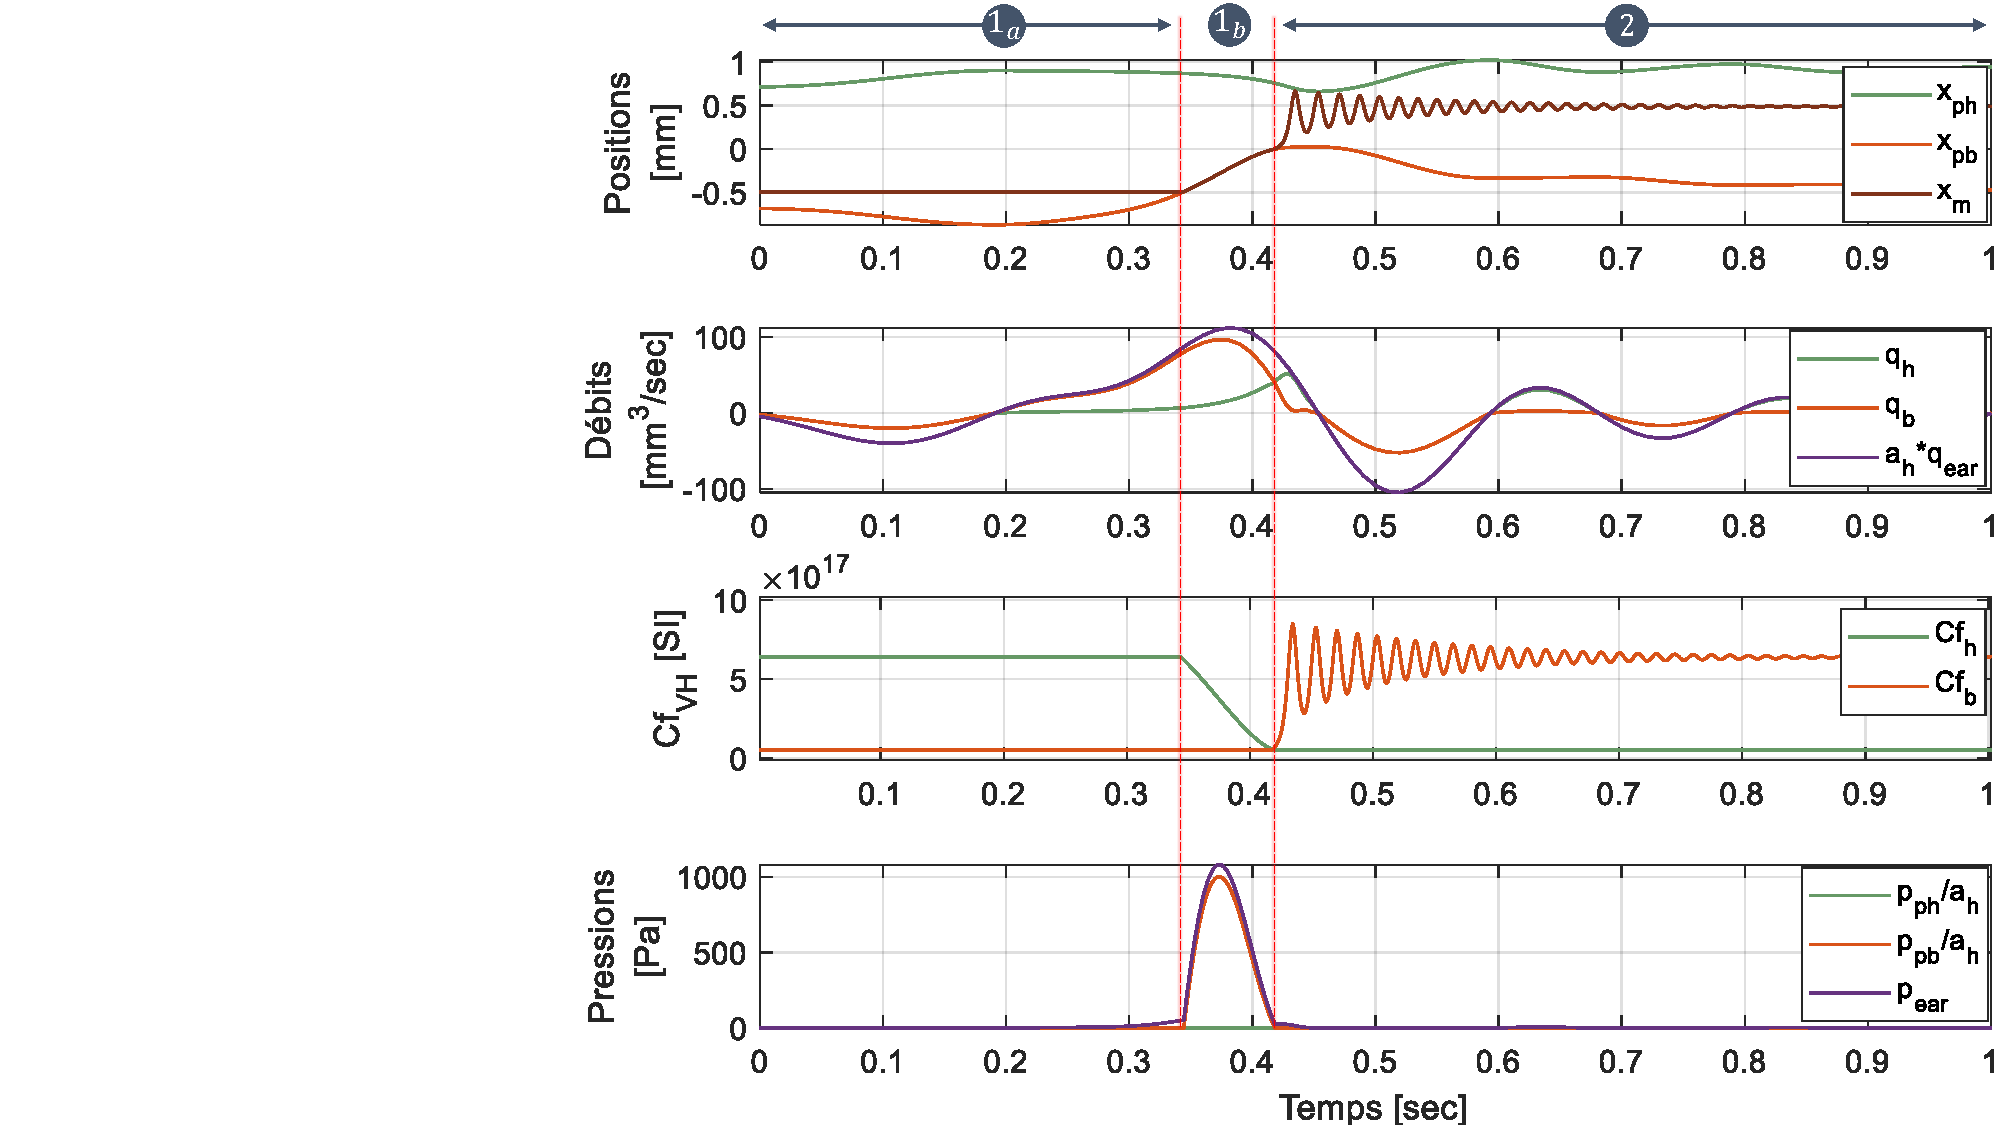
\includegraphics[trim={9.8cm 0cm 0cm 0cm},clip,width=0.85\textwidth]{../Chap2/Figure/simu_pos_debit_Cf_pression_1CYCLE.pdf}
	\caption{Résultats de simulation pour les positions, débits, Coefficient de PdC et pressions en concordance de temps}
	\label{fig:simu_pos_debit_Cf_pression_1CYCLE}
\end{center}	
\end{figure}
%%%%%%%%%%%%%%%%%%%%%%%%%%%%%%%%%%%%%%%%%

Le déplacement de volume découlant du travail mécanique de la fermeture de la mâchoire a lieu durant l'intervalle $t\in [0,2 - 0,45]s$. La mâchoire se trouve en position fermée à $t\approx 0.45s$ lorsque le débit s'annule. La variation de débit après la fermeture de la mâchoire découle de l'impédance imposée à la pompe lors des mesures de $\Delta V_{ear}$ sur une oreille humaine. En effet, ces données expérimentales sont issues du mouvement de l'aimant mobile dans le récupérateur hydro-électromagnétique illustré sur la figure \ref{fig:Critias_electromag_schema}. La dynamique de $q_{ear}$ sera probablement différente une fois passée la fermeture de la mâchoire. On choisit néanmoins de garder ces données afin que la valeur moyenne du volume déplacé sur un cycle de mastication soit nulle, en accord avec la conservation de masse du point de vue du fluide entrant/sortant du bouchon d'oreille. 

L'évolution oscillatoire de $Cf_b$ découle de l'hypothèse que la VH$_b$ est solidaire de M durant la phase de récupération (éq. \ref{eq:Cf(x_m) evolution lineaire}). On constate qu'à $x=0$, $Cf_b = Cf_h = Cf_0$ et donc les deux pistons sont alimentés au travers des deux VHs ouvertes. Cependant, la masse franchit tout de même la barrière de potentiel car elle arrive près de $x=0$ avec une énergie cinétique non nulle et suffisante pour assurer le basculement de l'OB. On peut par ailleurs estimer la puissance fournie par le gisement hydraulique avec les niveaux de débits et de pressions.  
%%%%%%%%%%%%%%%%%%%%%%%%%%%%%%%%%%%%%%%%%
\begin{figure}[!h]
\begin{center}
    \captionsetup{justification=centering}
	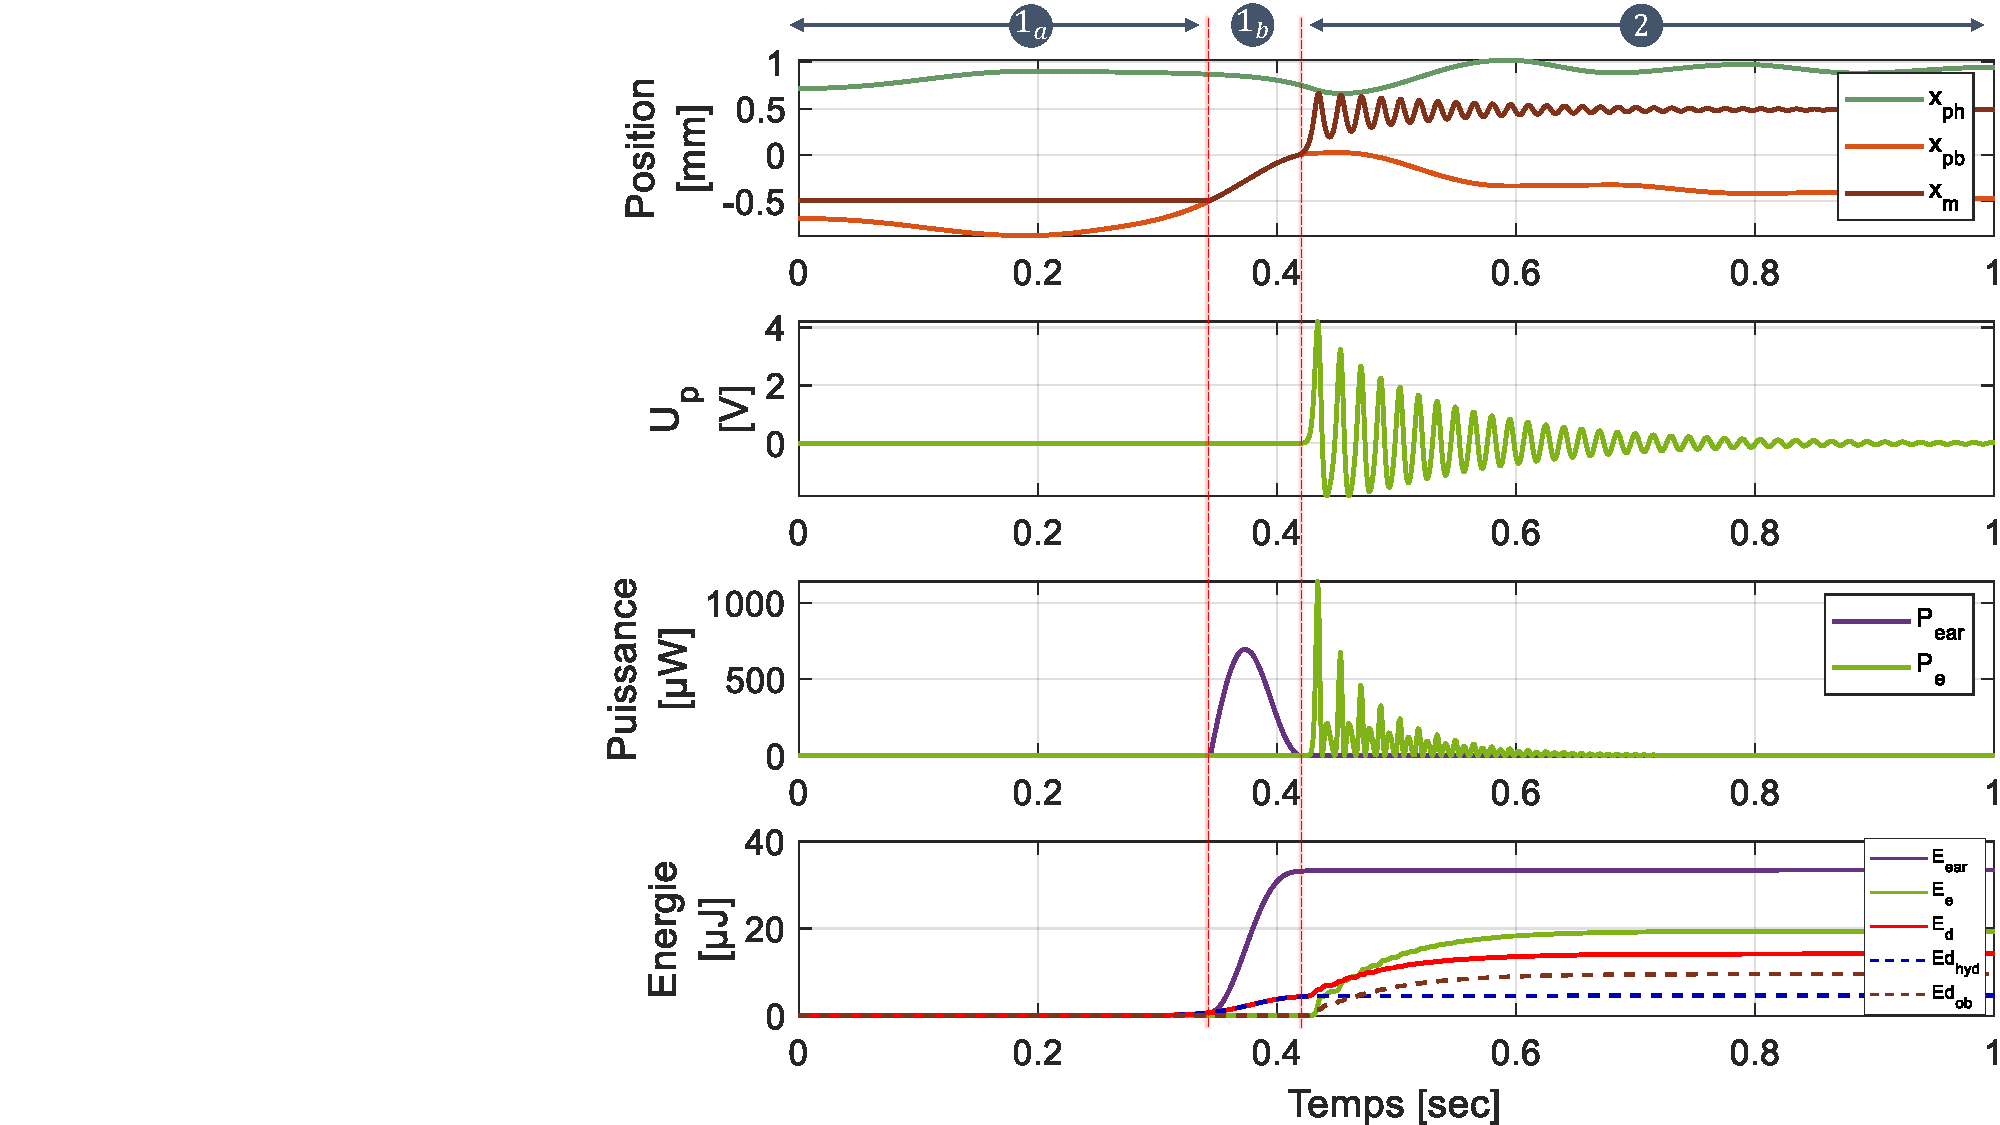
\includegraphics[trim={10cm 0cm 0cm 0cm},clip,width=0.8\textwidth]{../Chap2/Figure/simu_pos_Up_puissances_energie_1CYCLE.pdf}
	\caption{Résultats de simulation pour les positions, tension GPA, puissances et énergies}
	\label{fig:simu_pos_Up_puissances_energie_1CYCLE}
\end{center}	
\end{figure}
%%%%%%%%%%%%%%%%%%%%%%%%%%%%%%%%%%%%%%%%%

Il est également possible de déduire, de la simulation, la figure \ref{fig:simu_pos_Up_puissances_energie_1CYCLE} qui montre l'évolution de la tension $U_p$ aux bornes du GPA, le bilan des puissances et le bilan énergétique. Il révèle qu'un tel système est théoriquement capable de récupérer l'énergie de déformation du conduit auditif avec un rendement global $\eta_g = 67.1\%$. 
%%%%%%%%%%%%%%%%%%%%		
\begin{figure}[!htbp]
	\begin{center}
		\captionsetup{justification=centering}
		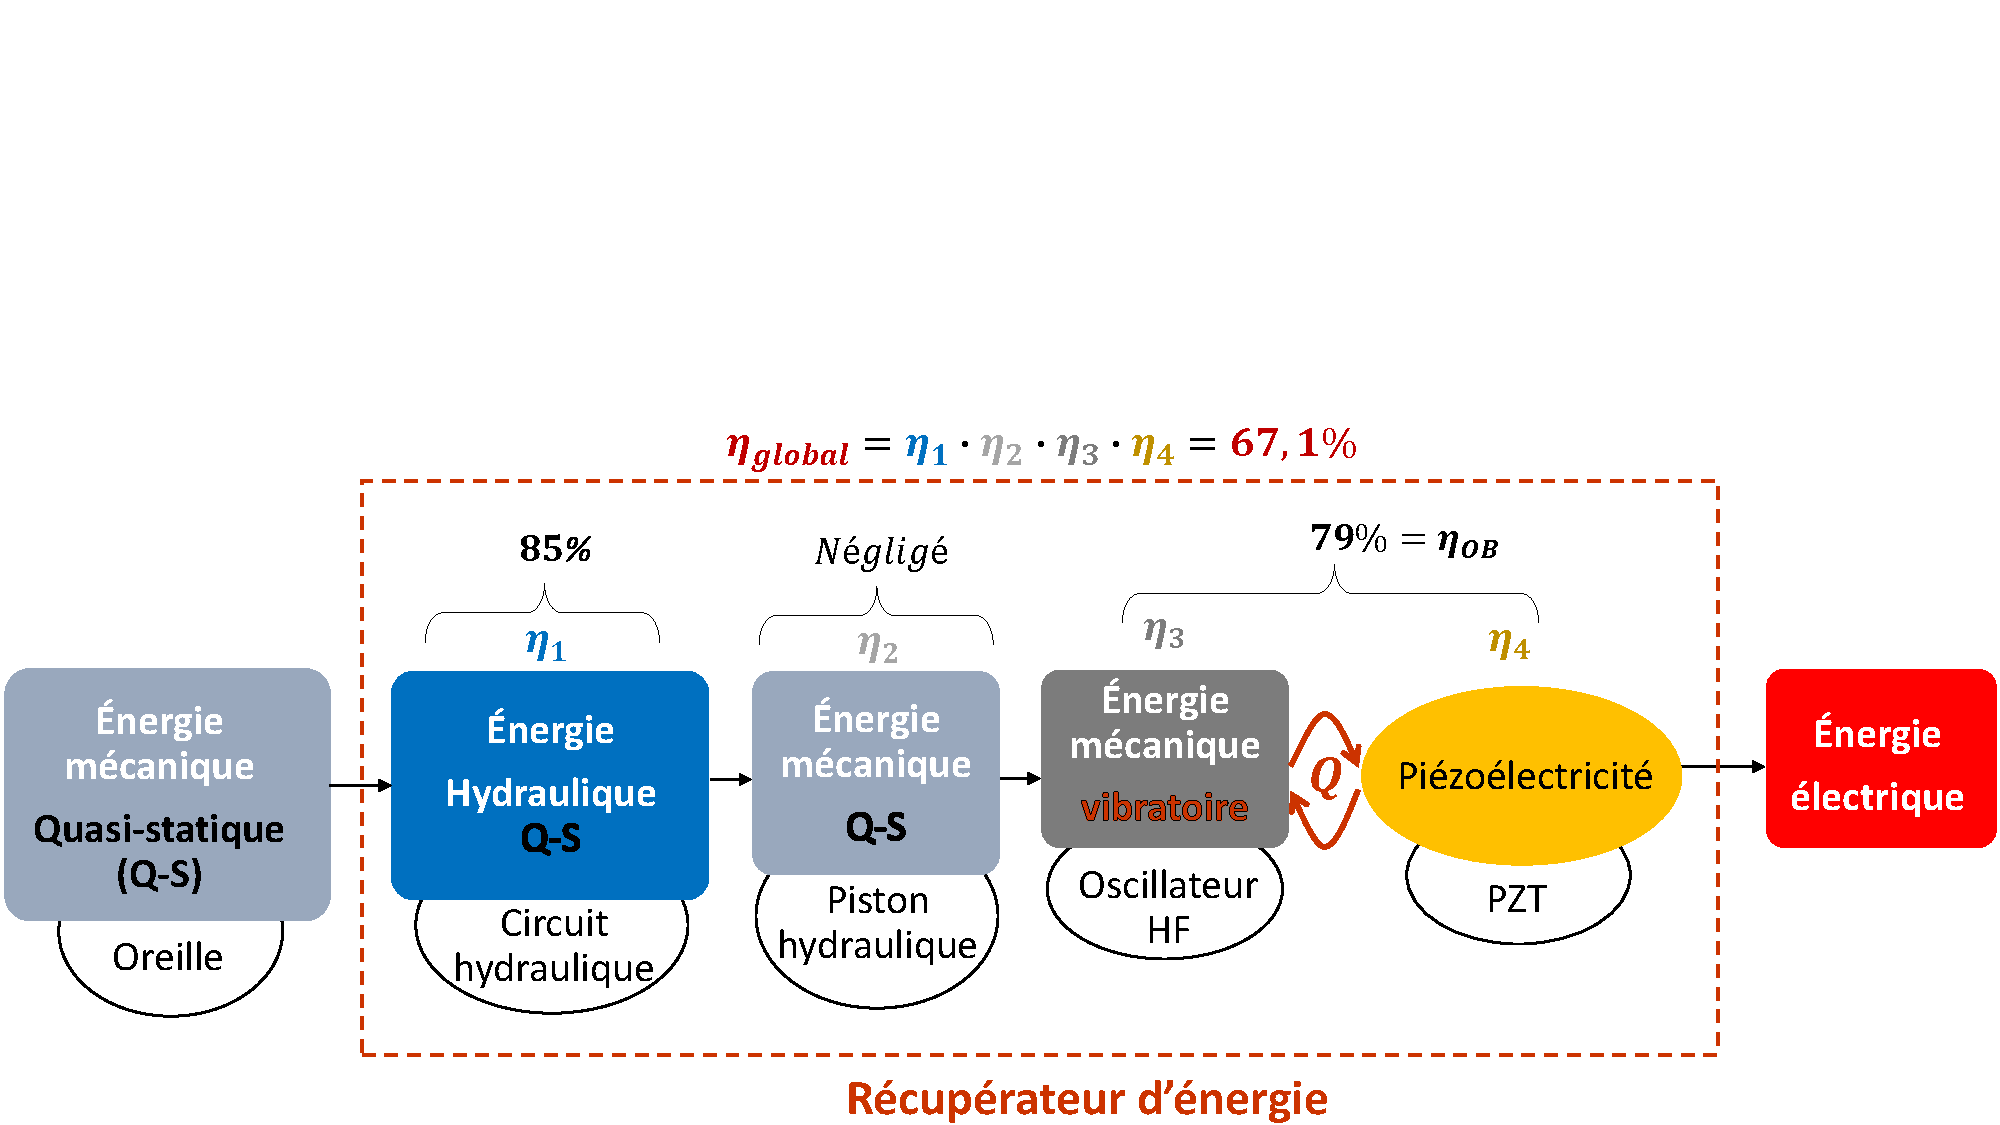
\includegraphics[trim={0cm 0cm 0cm 7cm},clip,width=\textwidth]{../Chap2/Figure/conversion_symme_rendements.pdf}
		\caption{Rendements estimés pour la chaîne de conversation envisagée dans ces travaux}
		\label{fig:conversion_symme_rendements_theoriques}
	\end{center}
\end{figure}
%%%%%%%%%%%%%%%%%%%%

La chaîne de conversion d'énergie théorique est présentée sur la figure \ref{fig:conversion_symme_rendements_theoriques} avec les données issues des simulations. Le rendement théorique de l'OB s'élève à $\eta_{OB} = 79$\% et celui du circuit hydraulique est estimé à $\eta_2 = 85$\% sans considérer les pertes par frottement et les pertes de charges dans la branche qui actionne.

Le prototype de bouchon d'oreille PVDF développé par Delnavaz \& Voix est capable de récupérer 70µW en moyenne sur un cycle de mastication (tab. \ref{tab:volume_protos_critias}). Notre solution, en revanche, est capable en théorie, de générer 33µW en moyenne, ce qui semble à première vue moins performant. Cela peut paraître surprenant au regard des rendements annoncés précédemment. Il est possible, cependant, d'apporter une explication à ces observations.

Tout d'abord, il faut noter qu'il n'y a pas eu de mesure de pression lors des essais réalisés avec le prototype de bouchon d'oreille équipé d'une bande PVDF. Cela rend difficile la comparaison des rendements, car l'énergie d'entrée n'est pas quantifiable pour ce prototype de récupérateur. De plus, le bouchon d'oreille piézoélectrique exploite l'énergie de flexion et l'énergie de compression dans le CA. Le récupérateur hydro-électromagnétique, lui, exploite seulement l'énergie de compression, avec une puissance moyenne générée de 0.3µW. Le système qu'on présente exploite, lui aussi, la seule source de compression. Il devrait donc, en théorie, fournir 100 fois plus d'énergie que le prototype hydro-électromagnétique. 

Ensuite, le dimensionnement du récupérateur introduit dans nos travaux a été réalisé avec une pression admissible de 1kPa, alors que l'oreille peut potentiellement supporter jusqu'à 12kPa \ref{tab:Bouchard_deltaPmax}. Une pression admissible plus importante offre une entrée énergétique d'autant plus grande et, par conséquent, une sortie de puissance d'autant plus importante. D'après l'énergie disponible dans l'oreille, estimée plus tôt avec l'équation \ref{eq:Energie_max_oreille}, notre système pourrait récupérer, avec les rendements actuels, 342µJ sur un cycle de mastication. En considérant une fréquence de mastication de 1.5Hz, il pourrait délivrer 513µW de puissance moyenne.

Le modèle numérique est incomplet à ce stade, car les rendements du découpleur, de l'amplificateur et des pistons hydrauliques ont été négligés. Il reste néanmoins prometteur pour une investigation expérimentale au vu des forts rendements estimés. Le prochain chapitre présente alors le dimensionnement, la conception, ainsi que la caractérisation de l'OB intégrant le GPA pour corréler le fonctionnement du modèle théorique.
